%--------------------Correction automatique

\section{Analyse de l'impact des corrections de ROC sur la REN}
\label{sec:COR-OCR-IMPACT-NER}

\textbf{Dans cette section, nous présentons l'outil Jamspell (Jspll) et les modèles de langue que nous utilisons pour la correction automatique des transcriptions de ROC bruitées. Nous proposons plusieurs manières d'évaluer des résultats de REN sur des  corrections automatiques de ROC bruitées. D'abord nous exposons une typologie des contaminations de corrections de ROC issues de l'analyse manuelle résultats. Bien que nous ayons déterminé qu'il s'agit d'une manière trop stricte d'évaluer la REN en contexte bruité nous réemployons les intersections. Nous utilisons  des mesures de distance textuelle pour mener une évaluation plus souple. Enfin, nous calculons la précision, le rappel et le F-score à l'aide de l'outil \textsc{Nerval}.}

\subsection{Outils de la correction des sorties ROC utilisés dans le cadre de cette étude}
\label{subsec:outils_COR-OCR-IMPACT-NER}
\textbf{Concernant la correction automatique des textes issus des transcriptions ROC, nous avons utilisé Jspll, un outil développé en Python qui exploite un modèle de langue trigramme statistique\footnote{Pour plus de détails sur ce modèle \textit{cf}. \url{https://habr.com/en/articles/346618/}.} (grain mot), dont une partie des fonctionnalités est mise à disposition gratuitement sur le web.
% \footnote{Malgré de nombreuses tentatives d'installation sur nos machines en local, nous avons dû nous résoudre à le faire tourner dans un environnement Google Colab.}
Si les modèles de langues pour le français et l'anglais sont accessibles gratuitement, le modèle portugais est disponible uniquement dans la version payante de Jspll, de fait cette option n'a pas été testée.
Nous avons entraîné un modèle de langue pour Jspll pour chacune des trois langues. Pour ce faire, nous avons sélectionné 40\% de chacun des corpus mis à disposition par ELTeC\footnote{\textbf{soit 4 millions de tokens pour chaque modèle. A VERIFIER}} et nous en avons exclu les textes utilisés pour notre étude.}

\textbf{Nous avons donc procédé aux évaluations des différentes configurations présentées dans le tableau \ref{tab:config}}.

\begin{table}[h!]
    \centering
   %\scriptsize{\begin{tabular}{|c|cc|cc|cc|cc|}
%
%\hline   
%ROC &  \multicolumn{2}{l|}{Kraken} &  \multicolumn{2}{l|}{Tess. en} & \multicolumn{2}{l|}{Tess. fr} &  \multicolumn{2}{l|}{Tess. pt} \\ 
%\hline
%REN & \textit{sp}} & \textit{st} & \textit{sp}} & \textit{st}&\textit{sp}} & \textit{st} &\textit{sp}} & \textit{st} \\
%\hline
%non corr. &\ding{51}} & \ding{51} & \ding{51}} & \ding{51}&\ding{51}} & \ding{51} &\ding{51}} & \ding{53} \\
%Jspll-pretr. &\ding{51}} & \ding{51} & \ding{51}} & \ding{51}&\ding{51}} & \ding{51} &\ding{53}} & \ding{53} \\
%Jspll-ELTeC  &\ding{51}} & \ding{51} & \ding{51}} & \ding{51}&\ding{51}} & \ding{51} &\ding{51}} &\ding{53}  \\
%  \hline
%\end{tabular}}

% \begin{tabular}{|c|cccc|}
% \hline
% ROC          & \multicolumn{1}{l|}{Kraken}                 & \multicolumn{1}{l|}{Tess. en}               & \multicolumn{1}{l|}{Tess. fr}               & \multicolumn{1}{l|}{Tess. pt} \\ \hline
% REN          & \multicolumn{4}{c|}{\textbackslash{}textttspaCy\_lg}                                                                                                                    \\ \hline
% non corr.    & \multicolumn{1}{c|}{\textbackslash{}ding51} & \multicolumn{1}{c|}{\textbackslash{}ding51} & \multicolumn{1}{c|}{\textbackslash{}ding51} & \textbackslash{}ding51        \\
% Jspll-pretr. & \multicolumn{1}{c|}{\textbackslash{}ding51} & \multicolumn{1}{c|}{\textbackslash{}\ding51 & \multicolumn{1}{c|}{\textbackslash{}ding51} & \textbackslash{}ding53        \\
% Jspll-ELTeC  & \multicolumn{1}{c|}{\textbackslash{}ding51} & \multicolumn{1}{c|}{\textbackslash{}ding51} & \multicolumn{1}{c|}{\textbackslash{}ding51} & \textbackslash{}ding51        \\ \hline
% \end{tabular}



% \scriptsize{\begin{tabular}{|c|c|c|c|c|}

% \hline   
% ROC &  Kraken &  Tess. en & Tess. fr &  Tess. pt \\ 
% \hline
% REN & \multicolumn{2}{c|}{\texttt{spaCy\_lg}} &  &  & \\
% % \hline
% non corr. &\ding{51} & \ding{51} &\ding{51} &\ding{51} \\
% Jspll-pretr. &\ding{51} & \ding{51} &\ding{51}&\ding{53} \\
% Jspll-ELTeC  &\ding{51} & \ding{51} &\ding{51}  &\ding{51}  \\
%   \hline
% \end{tabular}}

\scriptsize{
\begin{tabular}{|c|cccc|}
\hline
ROC          & \multicolumn{1}{l|}{Kraken}                 & \multicolumn{1}{l|}{Tess.en}               & \multicolumn{1}{l|}{Tess.fr}               & \multicolumn{1}{l|}{Tess.pt} \\ \hline
REN          & \multicolumn{4}{c|}{\texttt{spaCy\_lg}}                                                                                                                    \\ \hline
non corr.    & \multicolumn{1}{c|}{\ding{51}} & \multicolumn{1}{c|}{\ding{51}} & \multicolumn{1}{c|}{\ding{51}} & \ding{51}        \\
Jspll-pretr. & \multicolumn{1}{c|}{\ding{51}} & \multicolumn{1}{c|}{\ding{51}} & \multicolumn{1}{c|}{\ding{51}} & \ding{53}        \\
Jspll-ELTeC  & \multicolumn{1}{c|}{\ding{51}} & \multicolumn{1}{c|}{\ding{51}} & \multicolumn{1}{c|}{\ding{51}} & \ding{51}        \\ \hline
\end{tabular}
}

    \caption{Ensemble des configurations que nous évaluons dans cette étude. \texttt{spaCy\_lg}: sp.}
    \label{tab:config}
\end{table}

\subsection{Typologie des contaminations de corrections de ROC issues de l'analyse manuelle}
\label{subsec:Typologie_COR-OCR-IMPACT-NER}

Notons le cas particulier de l'EN ``Meunet-sur-Vatan'' dont les déclinaisons différentes en fonction du type de correcteur automatique sont indiquées dans le tableau \ref{tab:erreurs_corr_ELTeCFra}. Nous nous apercevons que les différentes versions de cette EN, contaminée par les différentes OCRisations et sur-corrections, n'ont pas du tout été extraites par \texttt{spaCy\_lg}.
%¨

\begin{table}[h!]
    \small
    \centering
   %%%%%%%%% Nouveau tableau sans stanza %%%%%%%%%%%


\begin{tabular}{|l|l|l|l|}

\hline

\bf{Version} & \bf {Contexte} & \bf{\texttt{spaCy\_lg}}\\
\hline 
Réf.\ & \textit{[\dots]  à l'assemblée de Meunet-sur-Vatan ;} & Meunet-sur-Vatan \\
 Kraken & \textit{[\dots]  \textcolor{red}{a} l'assem\textcolor{red}{h}l\textcolor{red}{6e'} de \textcolor{red}{N}eunet-sur-
\textcolor{red}{Y}atan'}& \textcolor{red}{Y}atan \\ 
 Kraken Jspll-fr &\textit{[\dots]  a l'assembl\textcolor{red}{6e'} de \textcolor{red}{N}eune\textcolor{red}{r}-sur-
\textcolor{red}{S}atan\textcolor{red}{'};}&\textcolor{red}{()} \\
  Kraken ELTeC-fr &\textit{[\dots]  a l'assem\textcolor{red}{h}l\textcolor{red}{6e'} de \textcolor{red}{N}eunet-sur-\textcolor{red}{Avant'};}&\textcolor{red}{()}\\


 %Tess & \textit{[\dots]  \textcolor{red}{4} l'assemblée\textcolor{red}{‘} de Meunet-sur-\textcolor{red}{y}Vatan\textcolor{red}{*}; } & \textcolor{red}{()} &Meunet-sur-\textcolor{red}{y}Vatan  \\
Tess fr &\textit{[\dots]  à l'assemblée\textcolor{red}{’} de Meunet-sur-\textcolor{red}{|} Vatan\textcolor{red}{*};  }& Meunet-sur-\textcolor{red}{|} \\
Tess fr Jspll-fr&\textit{[\dots]  à l'assemblée\textcolor{red}{’} de Meu\textcolor{red}{r}et-sur-
\textcolor{red}{|} Vatan\textcolor{red}{*};}&\textcolor{red}{()} \\
Tess fr ELTeC-fr& \textit{[\dots]  à l'assemblée\textcolor{red}{’} de Meunet-sur-\textcolor{red}{|} Vatan\textcolor{red}{*};}&Meunet-sur\textcolor{red}{\_}\\
\hline
\end{tabular}


%%%%%%%%% Ancien tableau avec stanza %%%%%%%%%%%%%

%\resizebox{\textwidth}{!}{
%\begin{tabular}{|l|l|l|l|l|l|}
%
%\hline
%
%\bf{Version} & \bf {Contexte} & \bf{\texttt{spaCy\_lg}}&\bf{\texttt{stanza}}\\
%\hline 
%Réf.\ & \textit{[\dots]  à l'assemblée de Meunet-sur-Vatan ;} & Meunet-sur-Vatan&Meunet-sur-Vatan \\
% Kraken & \textit{[\dots]  \textcolor{red}{a} l'assem\textcolor{red}{h}l\textcolor{red}{6e'} de \textcolor{red}{N}eunet-sur-
%\textcolor{red}{Y}atan'}& \textcolor{red}{Y}atan&\textcolor{red}{N}eunet-sur-
%\textcolor{red}{Y}atan \\ 
% Kraken Jspll-fr &\textit{[\dots]  a l'assembl\textcolor{red}{6e'} de \textcolor{red}{N}eune\textcolor{red}{r}-sur-
%\textcolor{red}{S}atan\textcolor{red}{'};}&\textcolor{red}{()}&\textcolor{red}{N}eune\textcolor{red}{r}-sur-
%\textcolor{red}{S}atan\\
%  Kraken ELTeC-fr &\textit{[\dots]  a l'assem\textcolor{red}{h}l\textcolor{red}{6e'} de \textcolor{red}{N}eunet-sur-\textcolor{red}{Avant'};}&\textcolor{red}{()}&\textcolor{red}{N}eunet-sur\textcolor{red}{\_}\\
%
%
% %Tess & \textit{[\dots]  \textcolor{red}{4} l'assemblée\textcolor{red}{‘} de Meunet-sur-\textcolor{red}{y}Vatan\textcolor{red}{*}; } & \textcolor{red}{()} &Meunet-sur-\textcolor{red}{y}Vatan  \\
%Tess fr &\textit{[\dots]  à l'assemblée\textcolor{red}{’} de Meunet-sur-\textcolor{red}{|} Vatan\textcolor{red}{*};  }& Meunet-sur-\textcolor{red}{|} &   Meunet-sur-\textcolor{red}{|} Vatan\\
%Tess fr Jspll-fr&\textit{[\dots]  à l'assemblée\textcolor{red}{’} de Meu\textcolor{red}{r}et-sur-
%\textcolor{red}{|} Vatan\textcolor{red}{*};}&\textcolor{red}{()}&Meu\textcolor{red}{r}et-sur-
%\textcolor{red}{|} Vatan\\
%Tess fr ELTeC-fr& \textit{[\dots]  à l'assemblée\textcolor{red}{’} de Meunet-sur-\textcolor{red}{|} Vatan\textcolor{red}{*};}&Meunet-sur\textcolor{red}{\_}&Meunet-sur-\textcolor{red}{|} Vatan\\
%\hline
%\end{tabular}
%}
     \caption{Exemples illustrant l'impact de la correction de la ROC sur la REN avec \texttt{spaCy\_lg}. {\normalfont La petite Jeanne}, Carraud.}
    \label{tab:erreurs_corr_ELTeCFra}
\end{table}

De façon similaire, nous observons dans le tableau \ref{tab:erreurs_corr_ELTeCEng} que le modèle de la correction automatique de ROC par Jspll, entraîné sur le corpus ELTeC, n'a pas eu d'impact sur l'extraction de l'EN ``Iudia'', puisqu'elle n'avait pas été corrigée en l'EN de référence ``India''. Par contre, le modèle Jspll pré-entraîné a bien corrigé la même EN, ce qui a permis son extraction sous forme correcte.
\begin{table}[h!]
\small
    \centering
   %%%%%%%%%%% Nouveau tableau sans stanza %%%%%%%%%%%

\begin{tabular}{|l|l|l|}

\hline

\bf{Version} & \bf {Contexte} & \bf{\texttt{spaCy\_lg}} \\
\hline 
Réf.\ &\textit{[...] before you went to India.} &India \\
 Kraken &\textit{[...] before you went to I\textcolor{red}{u}dia.}&I\textcolor{red}{u}dia \\ 
 Kraken Jspll-en &\textit{[...] before you went to India}&India \\ 
 Kraken ELTeC-en &\textit{[...] before you went to I\textcolor{red}{u}dia.}&I\textcolor{red}{u}dia \\ 
% Tess &\textit{[...] before you went to India.}&India& India\\
 % Tess jspl &\textit{[...] before you went to India.}&India& India\\
  % Tess ELTeC &\textit{[...] before you went to India.}&India& India\\

\hline
\end{tabular}


%%%%%%%% Ancien tableau avec stanza %%%%%%%%%%%

%\begin{tabular}{|l|l|l|l|l|l|}
%
%\hline
%
%\bf{Version} & \bf {Contexte} & \bf{\texttt{spaCy\_lg}}&\bf{\texttt{stanza}}\\
%\hline 
%Réf.\ &\textit{[...] before you went to India.} &India &India \\
% Kraken &\textit{[...] before you went to I\textcolor{red}{u}dia.}&I\textcolor{red}{u}dia&I\textcolor{red}{u}dia\\ 
% Kraken Jspll &\textit{[...] before you went to India}&India &India\\ 
% Kraken ELTeC &\textit{[...] before you went to I\textcolor{red}{u}dia.}&I\textcolor{red}{u}dia&I\textcolor{red}{u}dia\\ 
%% Tess &\textit{[...] before you went to India.}&India& India\\
% % Tess jspl &\textit{[...] before you went to India.}&India& India\\
%  % Tess ELTeC &\textit{[...] before you went to India.}&India& India\\
%
%\hline
%\end{tabular}

    \caption{Exemples illustrant l'impact de la correction de ROC sur la REN avec \texttt{spaCy\_lg}. {\normalfont Vanity Fair}, Thackeray.}
    \label{tab:erreurs_corr_ELTeCEng}
\end{table}

%\begin{table}
%\small
 %   \centering
  % \begin{tabular}{|l|p{4cm}|l|l|l|}
%p{0.5cm}
\hline
\bf{Version} & \bf {Contexte} & \bf{\texttt{spaCy\_lg}}&\bf{\texttt{stanza}}\\
\hline
Réf.\ & \textit{Alegre Inglaterra! oh! alegre Inglaterra!} &Alegre Inglaterra &  N/A\\
&  &Inglaterra &  N/A\\
\hline
 Kraken &\textit{Alegre Inglate\textcolor{red}{n- }ra\textcolor{red}{l} oh\textcolor{red}{l} alegre Inglat\textcolor{red}{l}erra\textcolor{red}{.l}} &Alegre Inglate\textcolor{red}{n-} &  N/A\\
& &\textcolor{red}{()}&  N/A\\ 
\hline
Kraken ELTeCpt  &\textit{Alegre Inglate\textcolor{red}{n- }ra\textcolor{red}{l} oh\textcolor{red}{l} alegre Inglat\textcolor{red}{l}erra\textcolor{red}{.l}} &Alegre Inglate\textcolor{red}{n-}   & N/A \\
& &  \textcolor{red}{()}& N/A \\
\hline
Tess pt  &\textit{Alegre Inglater\textcolor{red}{-} ra\textcolor{red}{l} oh! alegre Inglaterra!} & Alegre Inglater\textcolor{red}{-} ra\textcolor{red}{l} oh! & N/A \\
& & Inglaterra & N/A \\
\hline
Tess pt ELTeCpt  & \textit{Alegre \textcolor{red}{Singular-} ral oh! alegre Inglaterra!}&Alegre \textcolor{red}{Singular-} ral oh!&N/A\\
& & Inglaterra & N/A \\

\hline
\end{tabular}


   % \caption{Exemples illustrant l'impact de la correction de ROC sur la REN avec \texttt{spaCy\_lg} et \texttt{stanza}, {\normalfont Uma familia ingleza}, Diniz.}
    %\label{tab:erreurs_corr_ELTeCPor}
%\end{table}


Nous nous appuyons également sur une typologie des corrections automatiques de ROC, résumée dans le tableau \ref{tab:res-analyses}, qui permet de distinguer les différents cas de figure où les corrections en question ont soit amélioré les sorties de ROC (MOBC), soit les ont incorrectement modifiées (MOMC, MOI, BOIC). 

\begin{table}[h!]
\small
    \centering
    \begin{tabular}{|l|l|}
%p{0.5cm}
\hline
 
Type Acronyme& Définition\\
\hline
MOBC & mal océrisées bien corrigées\\

\hline
MOMC& mal océrisées mal corrigées\\

\hline
MOI&mal océrisées ignorées \\
\hline
BOIC&  bien océrisées indûment corrigées \\
\hline
\end{tabular}



    \caption{Typologie de l'impact de la correction de ROC sur la REN.  }
    \label{tab:res-analyses}
\end{table}

Quelques exemples sont visibles dans le tableau \ref{tab:typologie_erreurs-corr_ELTeCEng}, 
% et \ref{tab:typologie_erreurs_corr_ELTeCFra}
parmi lesquels se distinguent les sur-corrections ``Conspire'' 
% et ``Earlier'' 
(au lieu de ``Devonshire'' 
% et ``Algiers''
dans ELTeC anglais), ainsi que ``Martincourt'' (au lieu de ``Morlincourt'' dans ELTeC français).

\begin{table}[h!]
\small
    \centering
   %%%%%%%%%%%% Nouveau tableau sans stanza %%%%%%%%%%%%%%

\resizebox{\textwidth}{!}{
\begin{tabular}{|l|l|l|l|}
%p{0.5cm}
\hline
% & \multicolumn{4}{c|}{TGB}\\\cline{2-5}
Type &Version & Contexte & \texttt{spaCy\_lg} \\
\hline
MOBC &Kraken &\textit{[…] when they were in Lon\textcolor{red}{l}on}&() \\
&Jspll&\textit{[…] when they were in London}&London \\
&ELTeC&\textit{[…] when they were in London}&London \\
\hline
MOMC& Kraken&\textit{[…] flowery
lanes peeuliar to \textcolor{red}{Dc}onshire;}&\textcolor{red}{Dc}onshire \\
&Jspll&\textit{[…] flowery
lanes peculiar to \textcolor{red}{Conspire};}&() \\
&ELTeC&\textit{[…] flowers
lanes peculiar to \textcolor{red}{Dc}onshire;}&\textcolor{red}{Dc}onshire \\
\hline
% MOI&Kraken&\textit{ […] dark woo\textcolor{red}{l} within
% ten miles of Oakwoo\textcolor{red}{l}.}& Oakwoo\textcolor{red}{l} &Oakwoo\textcolor{red}{l}\\
% &Jspll&\textit{[…] dark woo\textcolor{red}{l} within
% ten miles of Oakwoo\textcolor{red}{l}.}&  Oakwoo\textcolor{red}{l}&Oakwoo\textcolor{red}{l}\\
% &ELTeC&\textit{ […] dark wool within
% ten miles of Oakwoo\textcolor{red}{l}.}& Oakwoo\textcolor{red}{l}&Oakwoo\textcolor{red}{l}\\
% \hline
% BOIC&Kraken&\textit{[…] which the bombardment of Algiers } &Algiers&Algiers\\
% &Jspll&\textit{[…] which the bombardment of Algiers}&Algiers&Algiers\\
% &ELTeC&\textit{[…] which the bombardment of\textbf{ Earlier}}&\textcolor{red}{()}&\textcolor{red}{()}\\
% \hline
MOI&Kraken& \textit{cure de M\textcolor{red}{l}orlincourt\textcolor{red}{l}}& M\textcolor{red}{l}orlincourt\textcolor{red}{l} \\
&Jspll-fr&\textit{cure de  M\textcolor{red}{l}orlincourt\textcolor{red}{l}} &   M\textcolor{red}{l}orlincourt\textcolor{red}{l} \\
&ELTeC-fr& \textit{cure de  M\textcolor{red}{l}orlincourt\textcolor{red}{l}}&  M\textcolor{red}{l}orlincourt\textcolor{red}{l} \\
\hline
BOIC&Kraken& \textit{en retournant
de Morlincourt} &Morlincourt \\
&Jspll-fr&\textit{en retournant
de\textbf{ Martincourt}} & \textbf{Martincourt} \\
&ELTeC-fr&\textit{en retournant
de Morlincourt} &Morlincourt \\
\hline
\end{tabular}
%\label{tab:typologie_erreurs-corr_ELTeCEng}
}

%%%%%%%%%%%%%% Ancien tableau avec stanza %%%%%%%%%%%%%%%%%

%\resizebox{\textwidth}{!}{
%\begin{tabular}{|l|l|l|l|l|}
%%p{0.5cm}
%\hline
%% & \multicolumn{4}{c|}{TGB}\\\cline{2-5}
%Type &Version & Contexte & \texttt{spaCy\_lg} &\texttt{stanza}\\
%\hline
%MOBC &Kraken &\textit{[…] when they were in Lon\textcolor{red}{l}on}&()&Lon\textcolor{red}{l}on\\
%&Jspll&\textit{[…] when they were in London}&London&London\\
%&ELTeC&\textit{[…] when they were in London}&London&London\\
%\hline
%MOMC& Kraken&\textit{[…] flowery
%lanes peeuliar to \textcolor{red}{Dc}onshire;}&\textcolor{red}{Dc}onshire&\textcolor{red}{Dc}onshire\\
%&Jspll&\textit{[…] flowery
%lanes peculiar to \textcolor{red}{Conspire};}&()&\textcolor{red}{Conspire}\\
%&ELTeC&\textit{[…] flowers
%lanes peculiar to \textcolor{red}{Dc}onshire;}&\textcolor{red}{Dc}onshire&\textcolor{red}{Dc}onshire\\
%\hline
%% MOI&Kraken&\textit{ […] dark woo\textcolor{red}{l} within
%% ten miles of Oakwoo\textcolor{red}{l}.}& Oakwoo\textcolor{red}{l} &Oakwoo\textcolor{red}{l}\\
%% &Jspll&\textit{[…] dark woo\textcolor{red}{l} within
%% ten miles of Oakwoo\textcolor{red}{l}.}&  Oakwoo\textcolor{red}{l}&Oakwoo\textcolor{red}{l}\\
%% &ELTeC&\textit{ […] dark wool within
%% ten miles of Oakwoo\textcolor{red}{l}.}& Oakwoo\textcolor{red}{l}&Oakwoo\textcolor{red}{l}\\
%% \hline
%% BOIC&Kraken&\textit{[…] which the bombardment of Algiers } &Algiers&Algiers\\
%% &Jspll&\textit{[…] which the bombardment of Algiers}&Algiers&Algiers\\
%% &ELTeC&\textit{[…] which the bombardment of\textbf{ Earlier}}&\textcolor{red}{()}&\textcolor{red}{()}\\
%% \hline
%MOI&Kraken& \textit{cure de M\textcolor{red}{l}orlincourt\textcolor{red}{l}}& M\textcolor{red}{l}orlincourt\textcolor{red}{l} & M\textcolor{red}{l}orlincourt\textcolor{red}{l}\\
%&Jspll-fr&\textit{cure de  M\textcolor{red}{l}orlincourt\textcolor{red}{l}} &   M\textcolor{red}{l}orlincourt\textcolor{red}{l}& M\textcolor{red}{l}orlincourt\textcolor{red}{l}\\
%&ELTeC-fr& \textit{cure de  M\textcolor{red}{l}orlincourt\textcolor{red}{l}}&  M\textcolor{red}{l}orlincourt\textcolor{red}{l}&  M\textcolor{red}{l}orlincourt\textcolor{red}{l} \\
%\hline
%BOIC&Kraken& \textit{en retournant
%de Morlincourt} &Morlincourt &Morlincourt \\
%&Jspll-fr&\textit{en retournant
%de\textbf{ Martincourt}} & \textbf{Martincourt} & \textbf{Martincourt} \\
%&ELTeC-fr&\textit{en retournant
%de Morlincourt} &Morlincourt &Morlincourt \\
%\hline
%\end{tabular}
%%\label{tab:typologie_erreurs-corr_ELTeCEng}
%}

%\begin{tabular}{|l|l|l|l|l|}
%p{0.5cm}
%\hline
 %& \multicolumn{4}{c|}{TGB}\\\cline{2-5}
%&OCR & Corr. & REN &REN corr.\\
%\hline
%MOBC &“[…] Sainl-Cyr”&“[…] Saint-Cyr”&Sainl-Cyr&Saint-Cyr\\

%\hline
%MOMC& “[…] Nîme”&“[…] Mîme”&Nîme&Mîme\\

%\hline
 %MOI& 
%“[…] SaintAntoine”&
%“[…] SaintAntoine”&
%SaintAntoine &
 %SaintAntoine\\
%\hline
%BOIC&  
%“[…] Pinde”&
%“[…] Inde”&
%Pinde&
%Et du sommet du Inde\\
%\hline
%\end{tabular}
    \caption{Exemples illustrant la typologie de l'impact de la correction de ROC sur la REN avec \texttt{spaCy\_lg}. Configuration : Jspll -- correction avec le modèle pré-entraîné de JamSpell, ELTeC -- correction avec le modèle entraîné sur une partie de chaque sous-corpus ELTeC. Formes de références des entités : London, Devonshire, Morlincourt. {\normalfont Home influence}, Aguillar et {\normalfont Mon village}, Adam.}
    \label{tab:typologie_erreurs-corr_ELTeCEng}
\end{table}

% Le MOI et BOIC de ce tableau a été déplacé dans le tableau 13 (on a fusionné les deux tableaux, donc on a le MOBC et le MOMC du tableau 13 et le MOI et le BOIC du tableau 14)

% \begin{table}[h!]
% \small
%     \centering
%    \begin{tabular}{|l|l|l|l|l|}
%p{0.5cm}
\hline
% & \multicolumn{4}{c|}{TGB}\\\cline{2-5}
Type &Version & Contexte & \texttt{spaCy-lg} &\texttt{stanza}\\
\hline
MOBC &Kraken &\textit{[…] ville que ce Paris\textcolor{red}{l} Ici}& Paris\textcolor{red}{l} Ici & () \\
&Jspll&\textit{[…] ville que ce \textbf{Paris} Ici}& Paris &Paris \\
&ELTeC&\textit{[…] ville que ce Paris\textcolor{red}{l} Ici} & Paris\textcolor{red}{l} Ici &() \\
\hline
MOMC& Kraken&\textit{l\textcolor{red}{n} no\textcolor{red}{e}e au Grand-\textcolor{red}{Hl}ail} &Grand-\textcolor{red}{Hl}ail &Grand-\textcolor{red}{Hl}ail \\
&Jspllfr&\textit{un note au Grand-\textcolor{red}{H}ail;} & \textcolor{red}{H}ail&\textcolor{red}{H}ail \\
&ELTeCfr& \textit{l\textcolor{red}{n} no\textcolor{red}{e}e au Grand-\textcolor{red}{Ai\_l};} & Grand-\textcolor{red}{Ai }&Grand-\textcolor{red}{Ai } \\
\hline
MOI&Kraken& \textit{cure de M\textcolor{red}{l}orlincourt\textcolor{red}{l}}& M\textcolor{red}{l}orlincourt\textcolor{red}{l} & M\textcolor{red}{l}orlincourt\textcolor{red}{l}\\
&Jspllfr&\textit{cure de  M\textcolor{red}{l}orlincourt\textcolor{red}{l}} &   M\textcolor{red}{l}orlincourt\textcolor{red}{l}& M\textcolor{red}{l}orlincourt\textcolor{red}{l}\\
&ELTeCfr& \textit{cure de  M\textcolor{red}{l}orlincourt\textcolor{red}{l}}&  M\textcolor{red}{l}orlincourt\textcolor{red}{l}&  M\textcolor{red}{l}orlincourt\textcolor{red}{l} \\
\hline
BOIC&Kraken& \textit{en retournant
de Morlincourt} &Morlincourt &Morlincourt \\
&Jspllfr&\textit{en retournant
de\textbf{ Martincourt}} & \textbf{Martincourt} & \textbf{Martincourt} \\
&ELTeCfr&\textit{en retournant
de Morlincourt} &Morlincourt &Morlincourt \\
\hline
\end{tabular}




%      \caption{Exemples illustrant la typologie de l'impact de la correction de ROC sur la REN avec \texttt{spaCy\_lg} et \texttt{stanza}. Configuration : Jspll - correction avec le modèle pré-entraîné de JamSpell, ELTeC - correction avec le modèle entraîné sur une partie du corpus ELTeC. Formes de références des entités : Paris, Grand-Bail, Morlincourt. {\normalfont Le petit chose}, Daudet, {\normalfont La petite Jeanne}, Carraud et {\normalfont Mon village}, Adam.}
%     \label{tab:typologie_erreurs_corr_ELTeCFra}
% \end{table}

%___Ce tableau est redondant, non (vu que l'on l'a développé dans le Tableau 18) ?
% \begin{table}
%     \centering
%    \begin{tabular}{|l|p{4cm}|l|l|l|}
%p{0.5cm}
\hline
\bf{Version} & \bf {Contexte} & \bf{\texttt{spaCy\_lg}}&\bf{\texttt{stanza}}\\
\hline
Réf.\ & \textit{Alegre Inglaterra! oh! alegre Inglaterra!} &Alegre Inglaterra &  N/A\\
&  &Inglaterra &  N/A\\
\hline
 Kraken &\textit{Alegre Inglate\textcolor{red}{n- }ra\textcolor{red}{l} oh\textcolor{red}{l} alegre Inglat\textcolor{red}{l}erra\textcolor{red}{.l}} &Alegre Inglate\textcolor{red}{n-} &  N/A\\
& &\textcolor{red}{()}&  N/A\\ 
\hline
Kraken ELTeCpt  &\textit{Alegre Inglate\textcolor{red}{n- }ra\textcolor{red}{l} oh\textcolor{red}{l} alegre Inglat\textcolor{red}{l}erra\textcolor{red}{.l}} &Alegre Inglate\textcolor{red}{n-}   & N/A \\
& &  \textcolor{red}{()}& N/A \\
\hline
Tess pt  &\textit{Alegre Inglater\textcolor{red}{-} ra\textcolor{red}{l} oh! alegre Inglaterra!} & Alegre Inglater\textcolor{red}{-} ra\textcolor{red}{l} oh! & N/A \\
& & Inglaterra & N/A \\
\hline
Tess pt ELTeCpt  & \textit{Alegre \textcolor{red}{Singular-} ral oh! alegre Inglaterra!}&Alegre \textcolor{red}{Singular-} ral oh!&N/A\\
& & Inglaterra & N/A \\

\hline
\end{tabular}


%      \caption{Exemples illustrant l'impact de la correction des OCR sur la REN avec spaCylg et stanza \textit{}, }
%     \label{tab:my_label}
% \end{table}


\subsection{Analyses quantitatives des contaminations de ROC et de leurs corrections}
\label{subsec:quantitative_COR-OCR-IMPACT-NER}
\subsubsection{La diminution des hapax comme indicateur de la performance de la correction automatique}
La colonne \textit{Brut} du tableau \ref{tab:ELTeC} montre qu'il y a globalement plus de types d'entités récupérées par \texttt{spaCy} sur Kraken (CER moyen :) que sur Tesseract (CER moyen :), ce qui vient étayer l'hypothèse que plus la qualité de la transcription est mauvaise plus les variations orthographiques des EN peuvent être nombreuses et plus il y a d'hapax dans les résultats de la REN. Nous venons à penser que si la correction automatique fonctionne bien le nombre des hapax sera réduit dans les sorties de REN, puisque la variabilité du vocabulaire sera réduite.

En partant de ce postulat, nous observons que :
\begin{itemize}
\item globalement il semble que la correction automatique ce soit mieux passée pour le corpus ELTeC-eng que pour ELTeC-fra.
\item les modèles Jspll pré-entraînés et entraînés sur ELTeC pour chaque langue permettent d'avoir des transcriptions d'une meilleure qualité que le texte brut car le nombre des types d'EN, donc des hapax, diminue.
\item les modèles pré-entrainés  et entraînés sur ELTeC seraient globalement plus efficaces sur kraken que sur Tesseract. Il y aurait un effet de seuil concernant la qualité des OCR au delà duquel la correction automatique serait moins efficace, autrement dit plus un OCR serait de bonne qualité moins la correction serait pertinente. 
\item la correction automatique avec Jspll ELTeC sur Tesseract pour le français voit le nombre des hapax augmenter donc il y aurait un problème dû à la correction automatique avec ce modèle, néanmoins les résultats avec le modèle Jspll-prétain ne semble pas non plus indiquer que la correction se soit très bien passée.
\end{itemize}
 
Enfin, concernant le corpus ELTeC portugais, comme nous l'avons souligné précédemment, nous avons extrait uniquement les EN corrigées avec notre modèle Jspll-ELTeC pour le portugais. La quantité d'EN reconnues est moindre que celle trouvée sur la sortie brute de ROC, donc la correction semble avoir été pertinente.
\begin{table}[h!]
    \centering
    \small
    % Please add the following required packages to your document preamble:
% \usepackage{multirow}
% \usepackage[table,xcdraw]{xcolor}
% If you use beamer only pass "xcolor=table" option, i.e. \documentclass[xcolor=table]{beamer}

% Please add the following required packages to your document preamble:
% \usepackage{multirow}
% \usepackage[table,xcdraw]{xcolor}
% If you use beamer only pass "xcolor=table" option, i.e. \documentclass[xcolor=table]{beamer}

%\begin{tabular}{|
%>{\columncolor[HTML]{FFFFFF}}c |
%>{\columncolor[HTML]{FFFFFF}}c 
%>{\columncolor[HTML]{FFFFFF}}c 
%>{\columncolor[HTML]{FFFFFF}}c |
%>{\columncolor[HTML]{FFFFFF}}c 
%>{\columncolor[HTML]{FFFFFF}}c 
%>{\columncolor[HTML]{FFFFFF}}c |}
%\hline
%\multicolumn{1}{|r|}{}
% &
%  \multicolumn{3}{c|}{Kraken} &
%  \multicolumn{3}{c|}{Tesseract} \\ \cline{2-7} 
%%\multirow{}{}{} &
%\multicolumn{1}{|r|}{}
%&
%  \multicolumn{1}{c|}{Brut} &
%  \multicolumn{1}{c|}{\begin{tabular}[c]{@{}c@{}}JamSpell\\ pré-entraîné\end{tabular}} &
%  \multicolumn{1}{c|}{\begin{tabular}[c]{@{}c@{}}JamSpell- \\ ELTeC\end{tabular}} &
%  \multicolumn{1}{c|}{Brut} &
%  \multicolumn{1}{c|}{\begin{tabular}[c]{@{}c@{}}JamSpell\\ pré-entraîné\end{tabular}} &
%  \multicolumn{1}{c|}{\begin{tabular}[c]{@{}c@{}}JamSpell- \\ ELTeC\end{tabular}} \\ \hline
%\multicolumn{1}{|r|}{Anglais}&
%  \multicolumn{1}{r|}{3 121} &
%  \multicolumn{1}{r|}{1 691, 54\%}&
%  \multicolumn{1}{r|}{1 446, 46\%}&
%  \multicolumn{1}{r|}{2 789} &
%  \multicolumn{1}{r|}{2 160, 77\%} &\multicolumn{1}{r|}{1 822, 65\%}
%   \\ \hline
%\multicolumn{1}{|r|}{Français} &
%  \multicolumn{1}{r|}{7 059} &
%  \multicolumn{1}{r|}{5 317, 75\%} &
%   \multicolumn{1}{r|}{\textbf{6 755, 95\%}}&
%  \multicolumn{1}{r|}{4 884} &
%  \multicolumn{1}{r|}{4 634, 95\%} &
%  \multicolumn{1}{r|}{\textbf{4 917, 100,7\%}} \\ \hline
%\multicolumn{1}{|r|}{Portugais} &
%  \multicolumn{1}{r|}{10 108} &
%  \multicolumn{1}{r|}{N/A} &
%  \multicolumn{1}{r|}{6 147} &
%  \multicolumn{1}{r|}{4 006} &
%  \multicolumn{1}{r|}{N/A} &
%  \multicolumn{1}{r|}{3 594} \\ \hline
%\end{tabular}

% Please add the following required packages to your document preamble:
% \usepackage{multirow}
\resizebox{\textwidth}{!}{
% Please add the following required packages to your document preamble:
% \usepackage{multirow}
%\begin{tabular}{|c|rrrrr|rrrrr|}
%\hline
%\multicolumn{1}{|l|}{\multirow{2}{*}{}} &
%  \multicolumn{5}{c|}{Kraken} &
%  \multicolumn{5}{c|}{Tesseract} \\ \cline{2-11} 
%\multicolumn{1}{|l|}{} &
%  \multicolumn{1}{c|}{Brut} &
%  \multicolumn{2}{c|}{\begin{tabular}[c]{@{}c@{}}JamSpell \\ pré-entraîné\end{tabular}} &
%  \multicolumn{2}{c|}{\begin{tabular}[c]{@{}c@{}}JamSpell-\\ ELTeC\end{tabular}} &
%  \multicolumn{1}{c|}{Brut} &
%  \multicolumn{2}{c|}{\begin{tabular}[c]{@{}c@{}}JamSpell\\ pré-entraîné\end{tabular}} &
%  \multicolumn{2}{c|}{\begin{tabular}[c]{@{}c@{}}JamSpell\\ ELTeC\end{tabular}} \\ \hline
%Anglais &
%  \multicolumn{1}{r|}{3 121} &
%  \multicolumn{1}{r|}{1 691} &
%  \multicolumn{1}{r|}{-46\%} &
%  \multicolumn{1}{r|}{1 446} &
%  -54\% &
%  \multicolumn{1}{r|}{2 789} &
%  \multicolumn{1}{r|}{2 160} &
%  \multicolumn{1}{r|}{-23\%} &
%  \multicolumn{1}{r|}{1 882} &
%  -35\% \\ \hline
%Français &
%  \multicolumn{1}{r|}{7 059} &
%  \multicolumn{1}{r|}{5 317} &
%  \multicolumn{1}{r|}{-25\%} &
%  \multicolumn{1}{r|}{\textbf{6 755}} &
%  \textbf{-5\%} &
%  \multicolumn{1}{r|}{4 884} &
%  \multicolumn{1}{r|}{4 634} &
%  \multicolumn{1}{r|}{-5\%} &
%  \multicolumn{1}{r|}{\textbf{4 917}} &
%  \textbf{+0,7\%} \\ \hline
%Portugais &
%  \multicolumn{1}{r|}{10 108} &
%  \multicolumn{1}{r|}{N/A} &
%  \multicolumn{1}{r|}{N/A} &
%  \multicolumn{1}{r|}{6 147} &
%   &
%  \multicolumn{1}{r|}{4 006} &
%  \multicolumn{1}{r|}{N/A} &
%  \multicolumn{1}{r|}{N/A} &
%  \multicolumn{1}{r|}{3 594} &
%   \\ \hline
%\end{tabular}
\begin{tabular}{|l|llrlr||llrlr|}
\hline
 &
  \multicolumn{5}{c||}{Kraken} &
  \multicolumn{5}{c|}{Tesseract} \\ \cline{2-11} 
\multirow{-2}{*}{} &
  \multicolumn{1}{c|}{Brut} &
  \multicolumn{2}{c|}{\begin{tabular}[c]{@{}c@{}}Jspll \\ pré-entraîné\end{tabular}} &
  \multicolumn{2}{c||}{\begin{tabular}[c]{@{}c@{}}Jspll-\\ ELTeC\end{tabular}} &
  \multicolumn{1}{c|}{Brut} &
  \multicolumn{2}{c|}{\begin{tabular}[c]{@{}c@{}}Jspll\\ pré-entraîné\end{tabular}} &
  \multicolumn{2}{c|}{\begin{tabular}[c]{@{}c@{}}Jspll\\ ELTeC\end{tabular}} \\ \hline\hline
\multicolumn{1}{|c|}{Anglais} &
  \multicolumn{1}{r|}{3 121} &
  \multicolumn{1}{r|}{1 691} &
  \multicolumn{1}{r|}{54\%} &
  \multicolumn{1}{r|}{1 446} &
  46\% &
  \multicolumn{1}{r|}{2 789} &
  \multicolumn{1}{r|}{2 160} &
  \multicolumn{1}{r|}{77\%} &
  \multicolumn{1}{r|}{1 882} &
  65\% \\ \hline
CER médian &
  \multicolumn{1}{c|}{0.364} &
  \multicolumn{2}{c|}{0.362} &
  \multicolumn{2}{c||}{0.364} &
  \multicolumn{1}{c|}{0.205} &
  \multicolumn{2}{c|}{0.261} &
  \multicolumn{2}{c|}{0.243} \\ \hline\hline
\multicolumn{1}{|c|}{Français} &
  \multicolumn{1}{r|}{7 059} &
  \multicolumn{1}{r|}{5 317} &
  \multicolumn{1}{r|}{75\%} &
  \multicolumn{1}{r|}{\textbf{6 755}} &
  \textbf{95\%} &
  \multicolumn{1}{r|}{4 884} &
  \multicolumn{1}{r|}{4 634} &
  \multicolumn{1}{r|}{95\%} &
  \multicolumn{1}{r|}{\textbf{4 917}} &
  \textbf{100,7\%} \\ \hline
CER médian & 
  \multicolumn{1}{c|}{0.098} &
  \multicolumn{2}{c|}{0.102} &
  \multicolumn{2}{c||}{0.104} &
  \multicolumn{1}{c|}{0.050} &
  \multicolumn{2}{c|}{0.053} &
  \multicolumn{2}{c|}{0.055} \\ \hline\hline
\multicolumn{1}{|c|}{Portugais} &
  \multicolumn{1}{r|}{10 108} &
  \multicolumn{1}{r|}{N/A} &
  \multicolumn{1}{r|}{N/A} &
  \multicolumn{1}{r|}{6 147} &
  61\% & 
  \multicolumn{1}{r|}{4 006} &
  \multicolumn{1}{r|}{N/A} &
  \multicolumn{1}{r|}{N/A} &
  \multicolumn{1}{r|}{3 594} &
  90\% \\ \hline
CER médian &
  \multicolumn{1}{c|}{0.159} &
  \multicolumn{2}{c|}{N/A} &
  \multicolumn{2}{c||}{0.155} &
  \multicolumn{1}{c|}{0.093} &
  \multicolumn{2}{c|}{N/A} &
  \multicolumn{2}{c|}{0.096} \\ \hline
\end{tabular}
}

    \caption{Nombre d'EN (types) avec les pourcentages d'EN issues des EN brutes et repérées par \texttt{spaCy\_lg} pour les sous-corpus ELTeC anglais, français et portugais. N/A -- modèle JamSpell pré-entrainé pour le portugais non disponible.}
    \label{tab:ELTeC}
\end{table}

\subsubsection{Calculs des intersections, toujours plus de problèmes d'alignements. }

Nous reprennons ici la stratégie d'évaluation stricte par calcul des intersections comme décrite dans la section \ref{subsec:inter_OCR-IMPACT-NER}.
Notre démarche évaluative est fondée sur l'intérêt de la correction automatique qui vise à diminuer le nombre de FP, ainsi qu'à augmenter l'intersection entre les EN de ROC et de référence. 

Les graphiques de la figure \ref{fig:intersection_globale-kraken} représentent les intersections entre les EN issues des textes de référence et celles provenant des versions de ROC (Kraken ou Tesseract) corrigées avec le modèle pré-entraîné de JamSpell (\ref{fig:ELTeCFRA_Kraken -- jspl-fr_spacy-lg-concat_intersection.png}-\ref{fig:ELTeCFRA_Tess. fr -- jspl-fr_spacy-lg-concat_intersection.png}), et le modèle entraîné avec le sous-corpus ELTeC français (\ref{fig:ELTeCFRA_Kraken -- jspl-ELTeCfr_spacy-lg-concat_intersection}-\ref{fig:ELTeCFRA_Tess -- jspl-ELTeCFR_spacy-lg-concat_intersection})

La figure \ref{fig:ELTeCFRA_Tess -- jspl-ELTeCFR_spacy-lg-concat_intersection} montre que le plus grand nombre d'EN en commun a été récupéré par \texttt{spaCy\_lg} quand le texte a été transcrit avec Tesseract et corrigé par le modèle entraîné sur le corpus ELTeC français.

 Il est notable que la correction automatique avec le modèle pré-entraîné de Jspll ou le modèle entraîné sur une partie du corpus ELTeC adapté à la langue du corpus testé ne sont pas un gain pour l'intersection. 
%%% INTERSECTIONS GLOBALES
\begin{figure}[h!]
    \begin{minipage}{7cm}
  \begin{subfigure}{1\textwidth}
  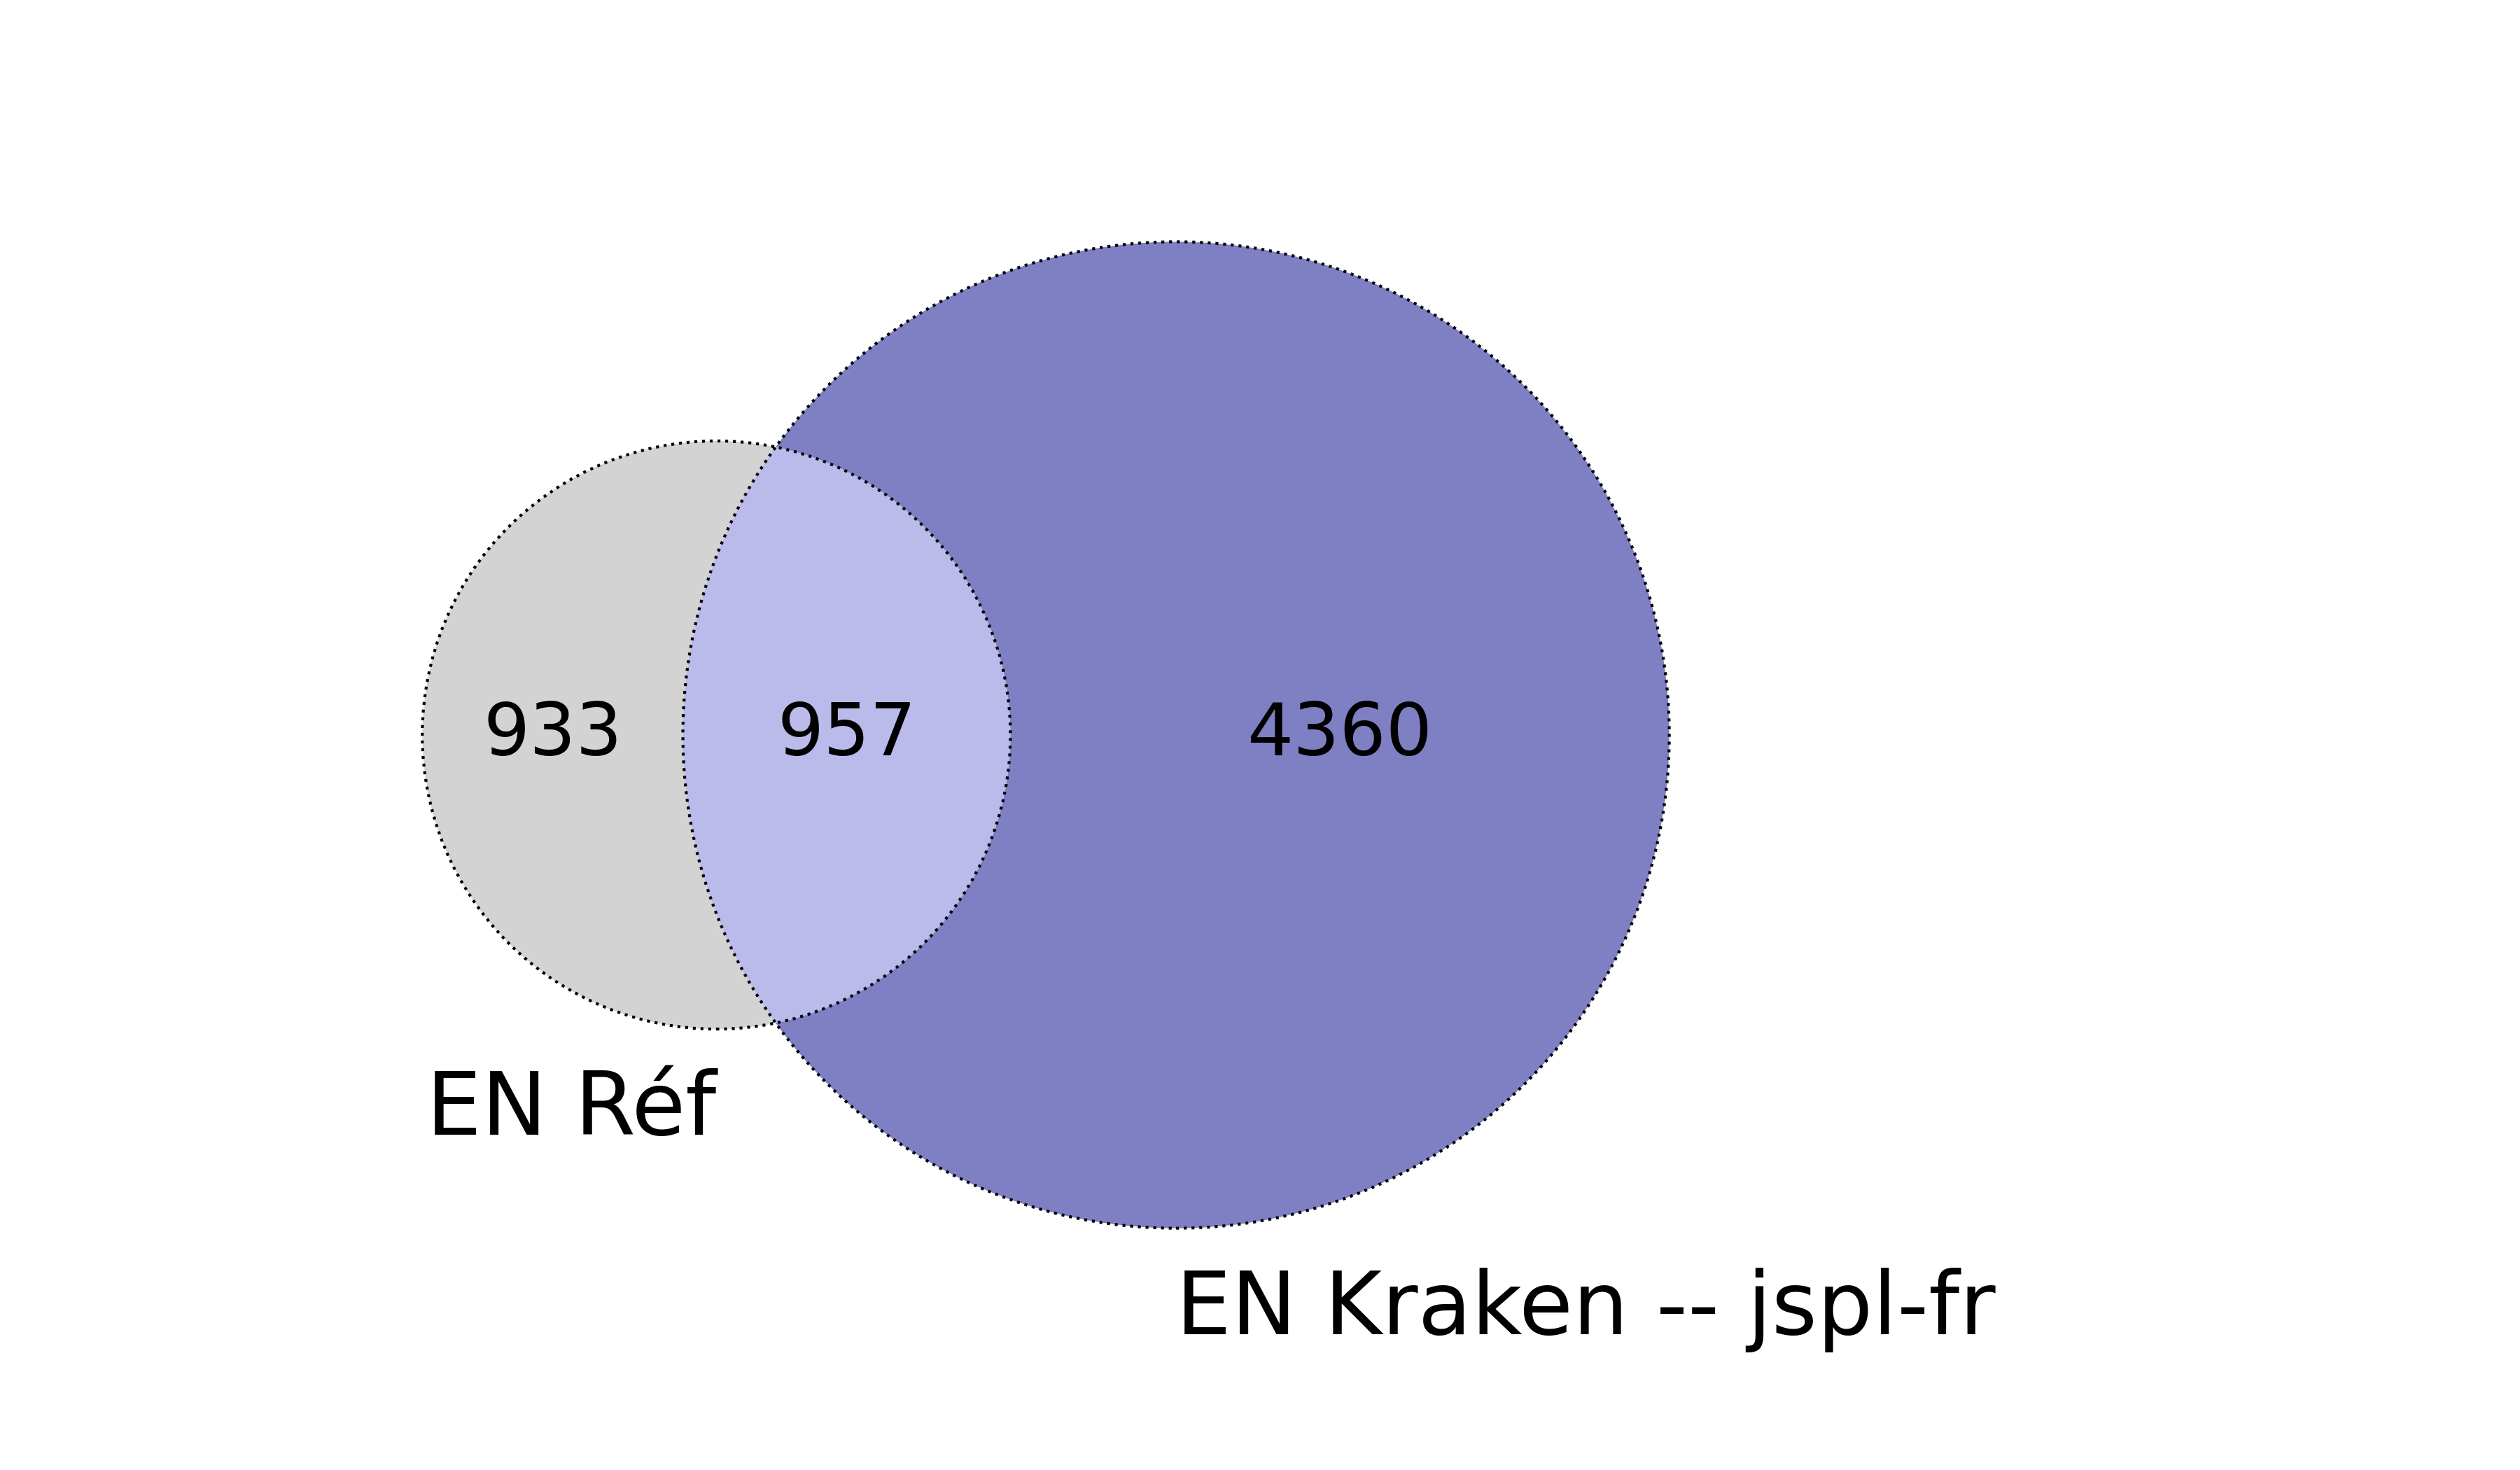
\includegraphics[width=1\textwidth]{IMAGES/INTERSECTIONS_GLOBALES/ELTeCFRA_Kraken -- jspl-fr_spacy-lg-concat_intersection.png} 
  \caption{Kraken corrigé Jspll pretrain --\texttt{spaCy\_lg}}
  \label{fig:ELTeCFRA_Kraken -- jspl-fr_spacy-lg-concat_intersection.png}
  \end{subfigure}
  \end{minipage}
  \begin{minipage}{7cm}
  \begin{subfigure}{1\textwidth}
  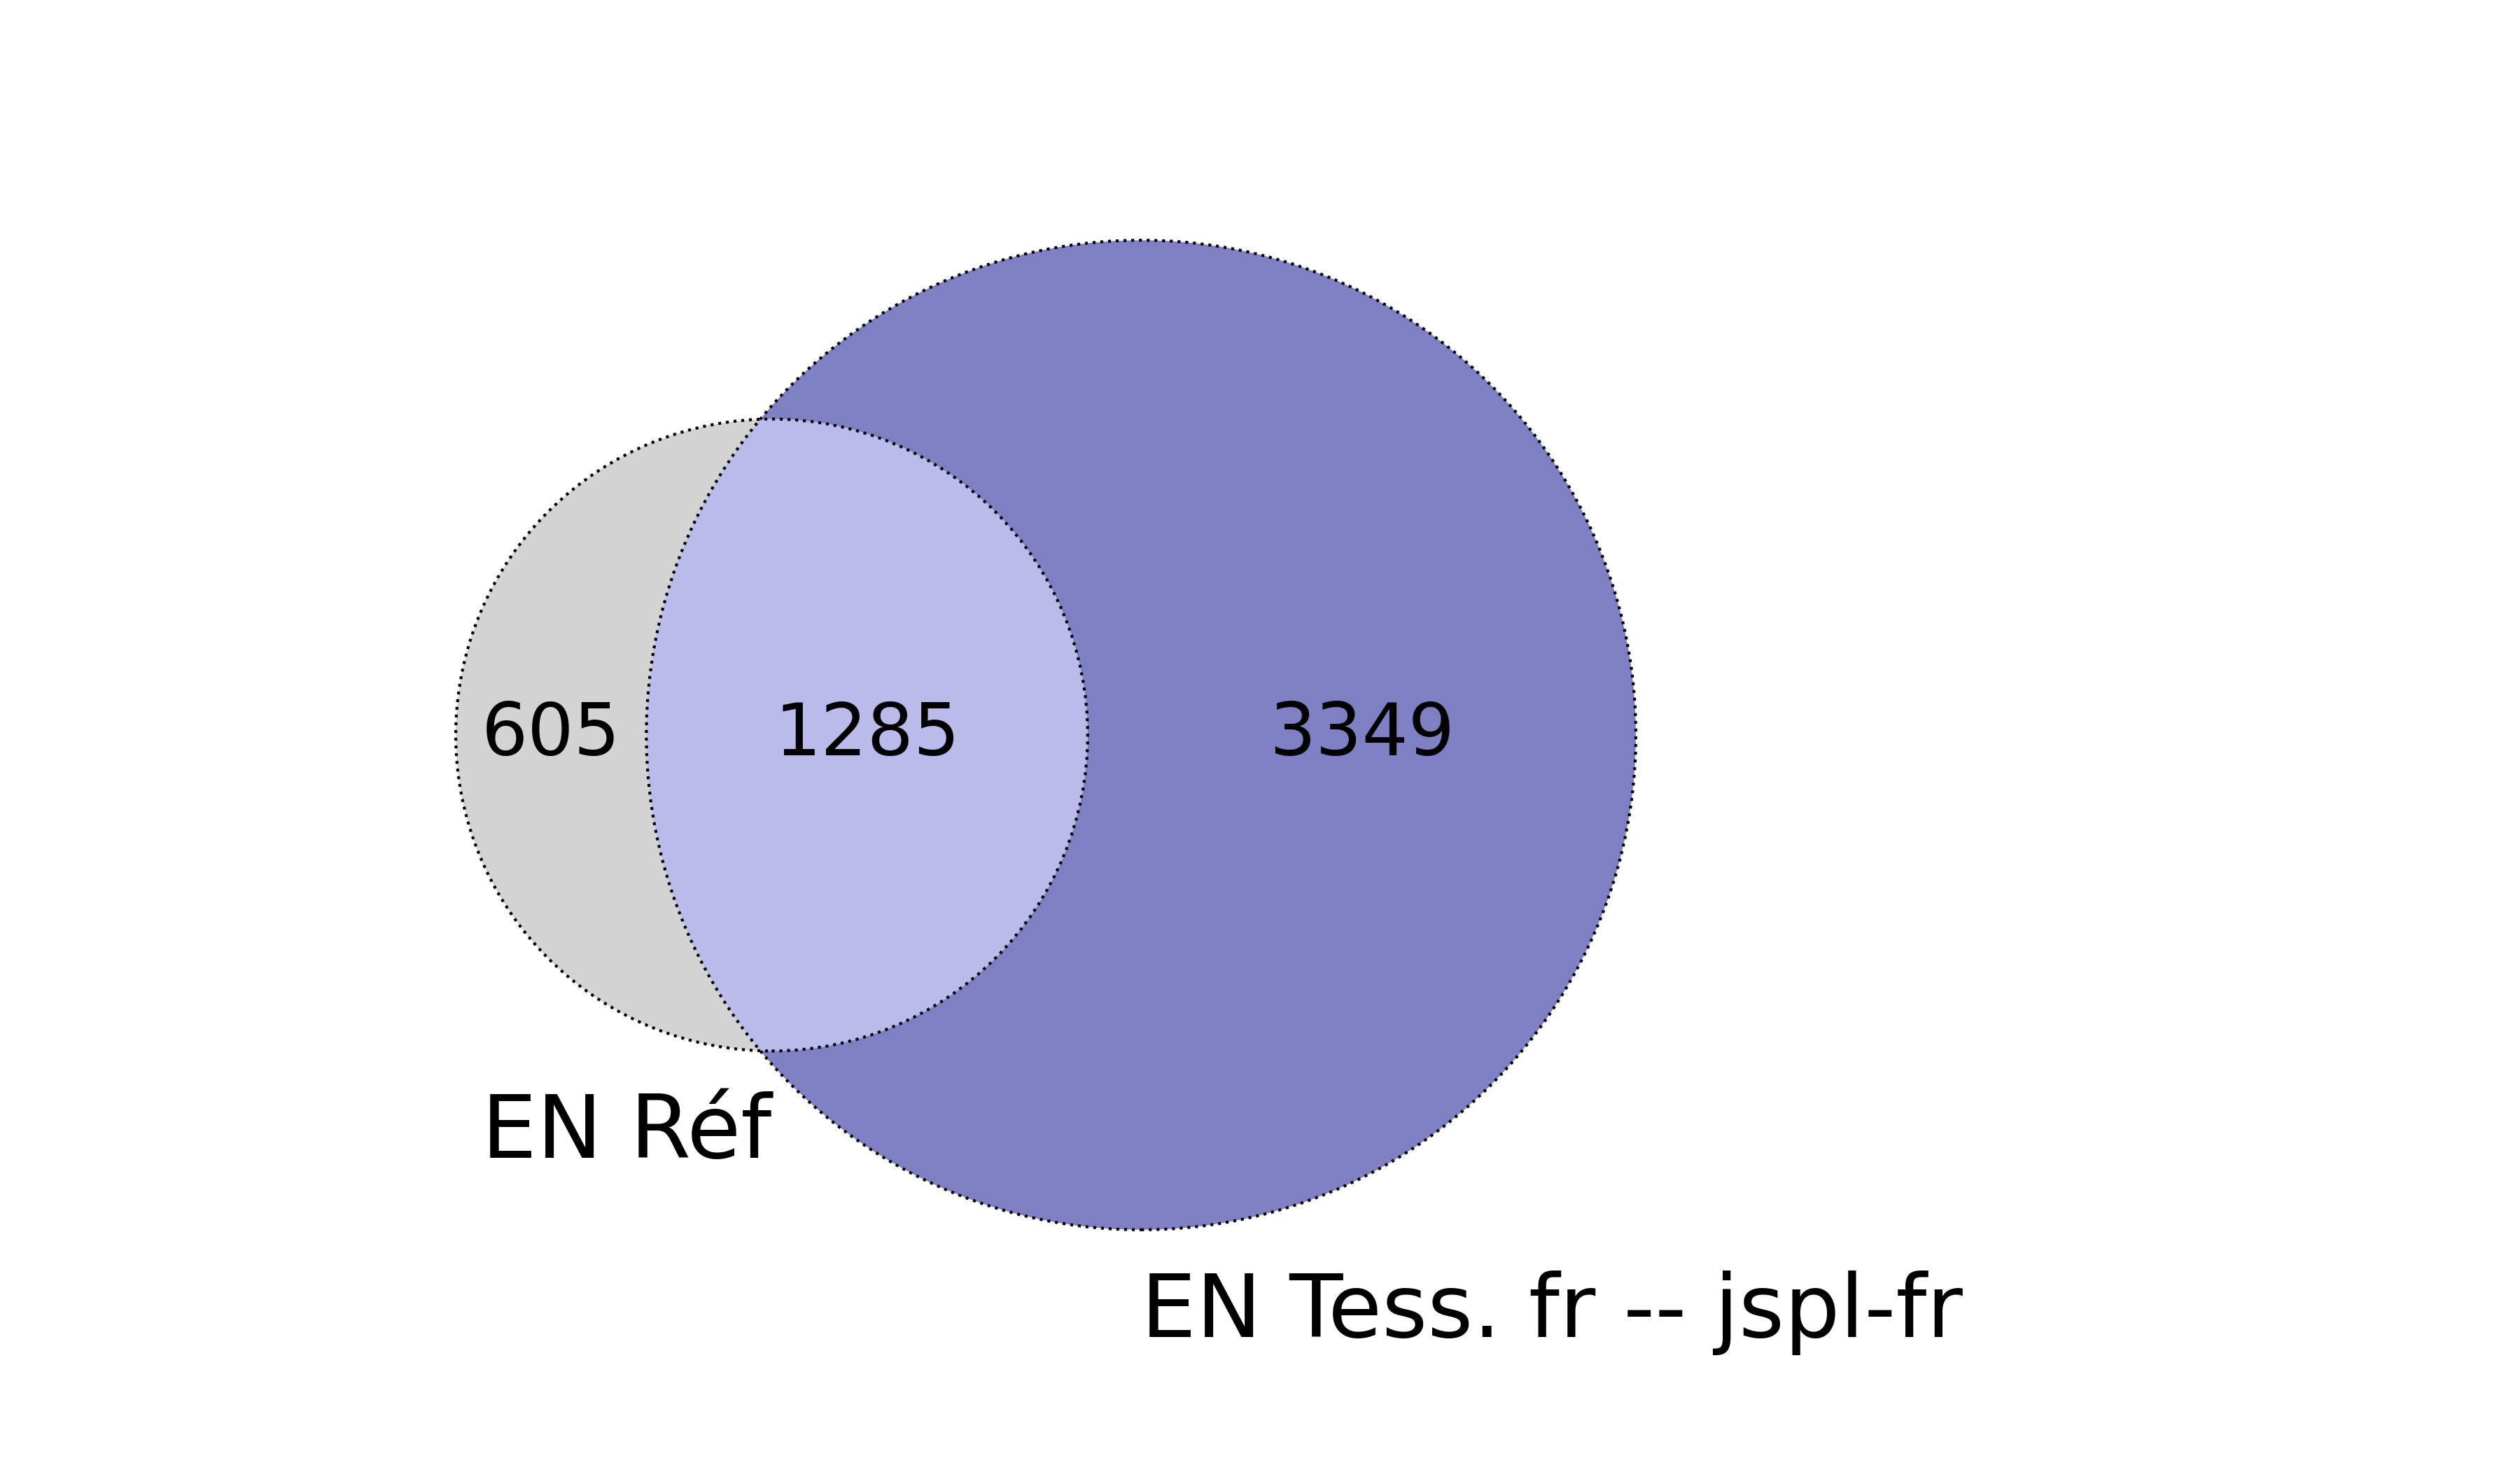
\includegraphics[width=1\textwidth]{IMAGES/INTERSECTIONS_GLOBALES/ELTeCFRA_Tess. fr -- jspl-fr_spacy-lg-concat_intersection.png} 
  \caption{Tess. fr. corrigé Jspll pretrain -- \texttt{spaCy\_lg}}
 \label{fig:ELTeCFRA_Tess. fr -- jspl-fr_spacy-lg-concat_intersection.png}
  \end{subfigure}
    \end{minipage}
\begin{minipage}{7cm}
  \begin{subfigure}{1\textwidth}
  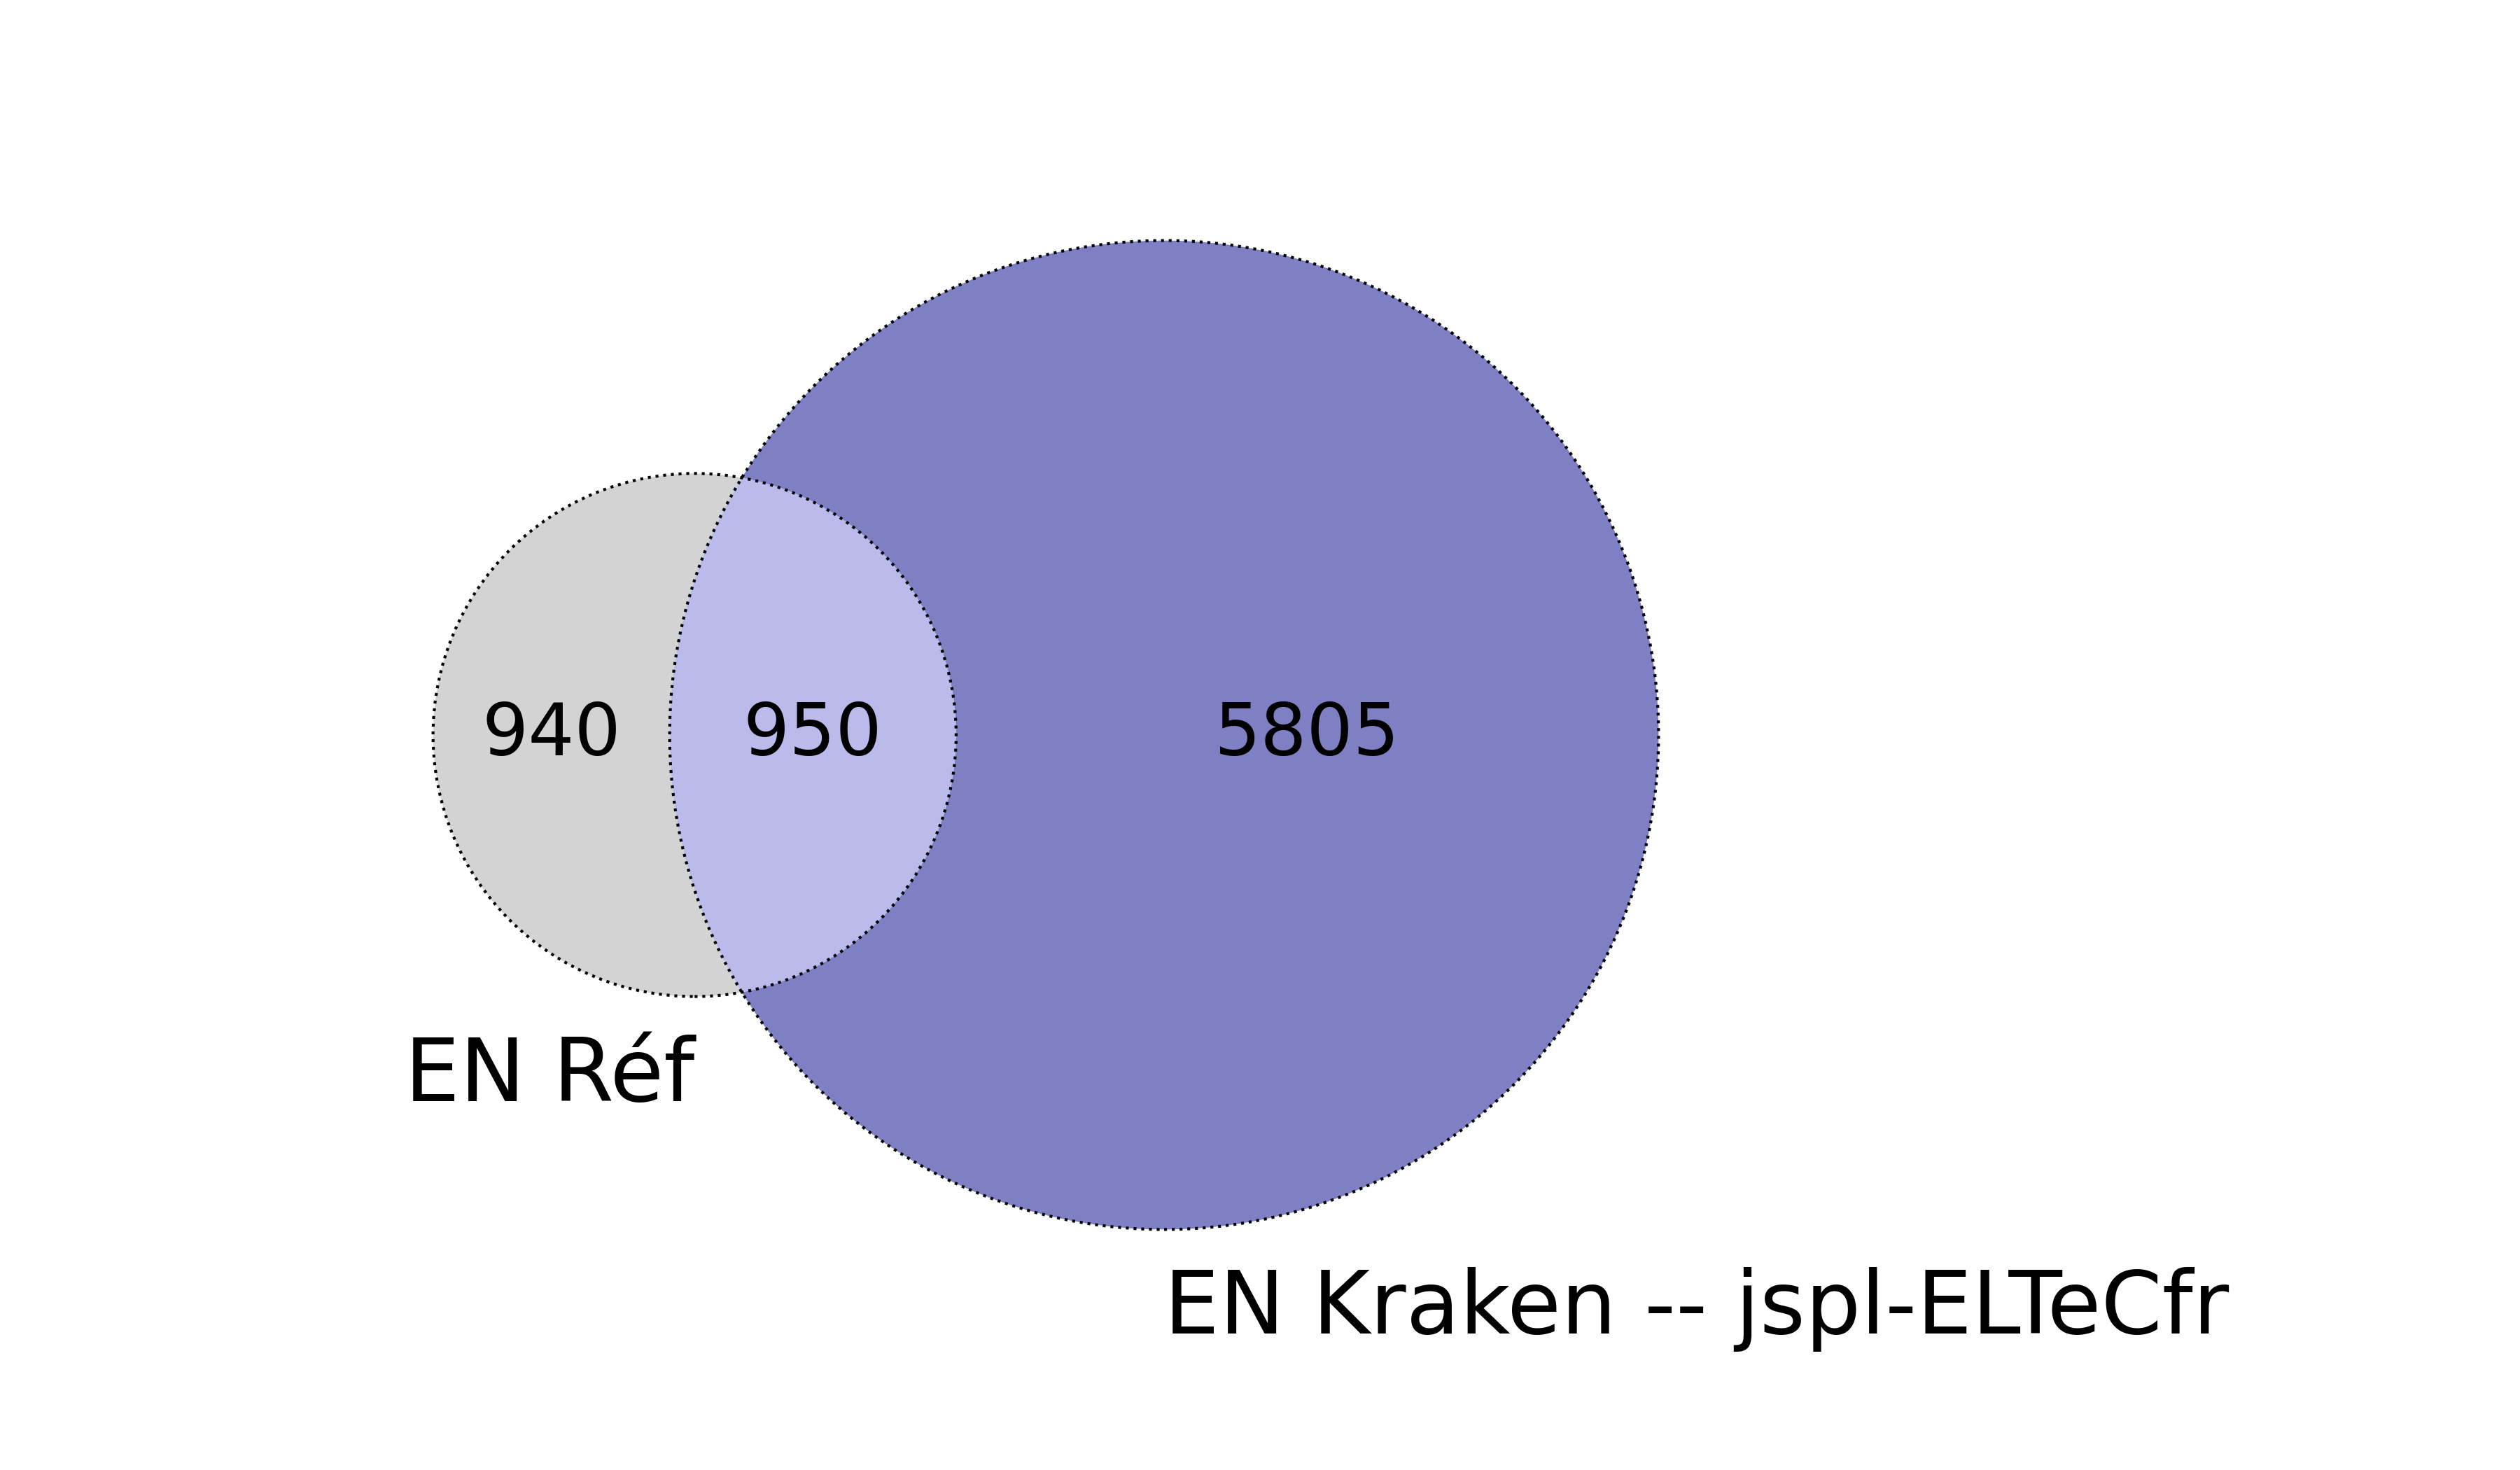
\includegraphics[width=1\textwidth]{IMAGES/INTERSECTIONS_GLOBALES/ELTeCFRA_Kraken -- jspl-ELTeCfr_spacy-lg-concat_intersection.png} 
  \caption{Kraken corrigé ELTeC-fr -- \texttt{spaCy\_lg}}
  \label{fig:ELTeCFRA_Kraken -- jspl-ELTeCfr_spacy-lg-concat_intersection}
  \end{subfigure}
  \end{minipage}
  \begin{minipage}{7cm}
  \begin{subfigure}{1\textwidth}
  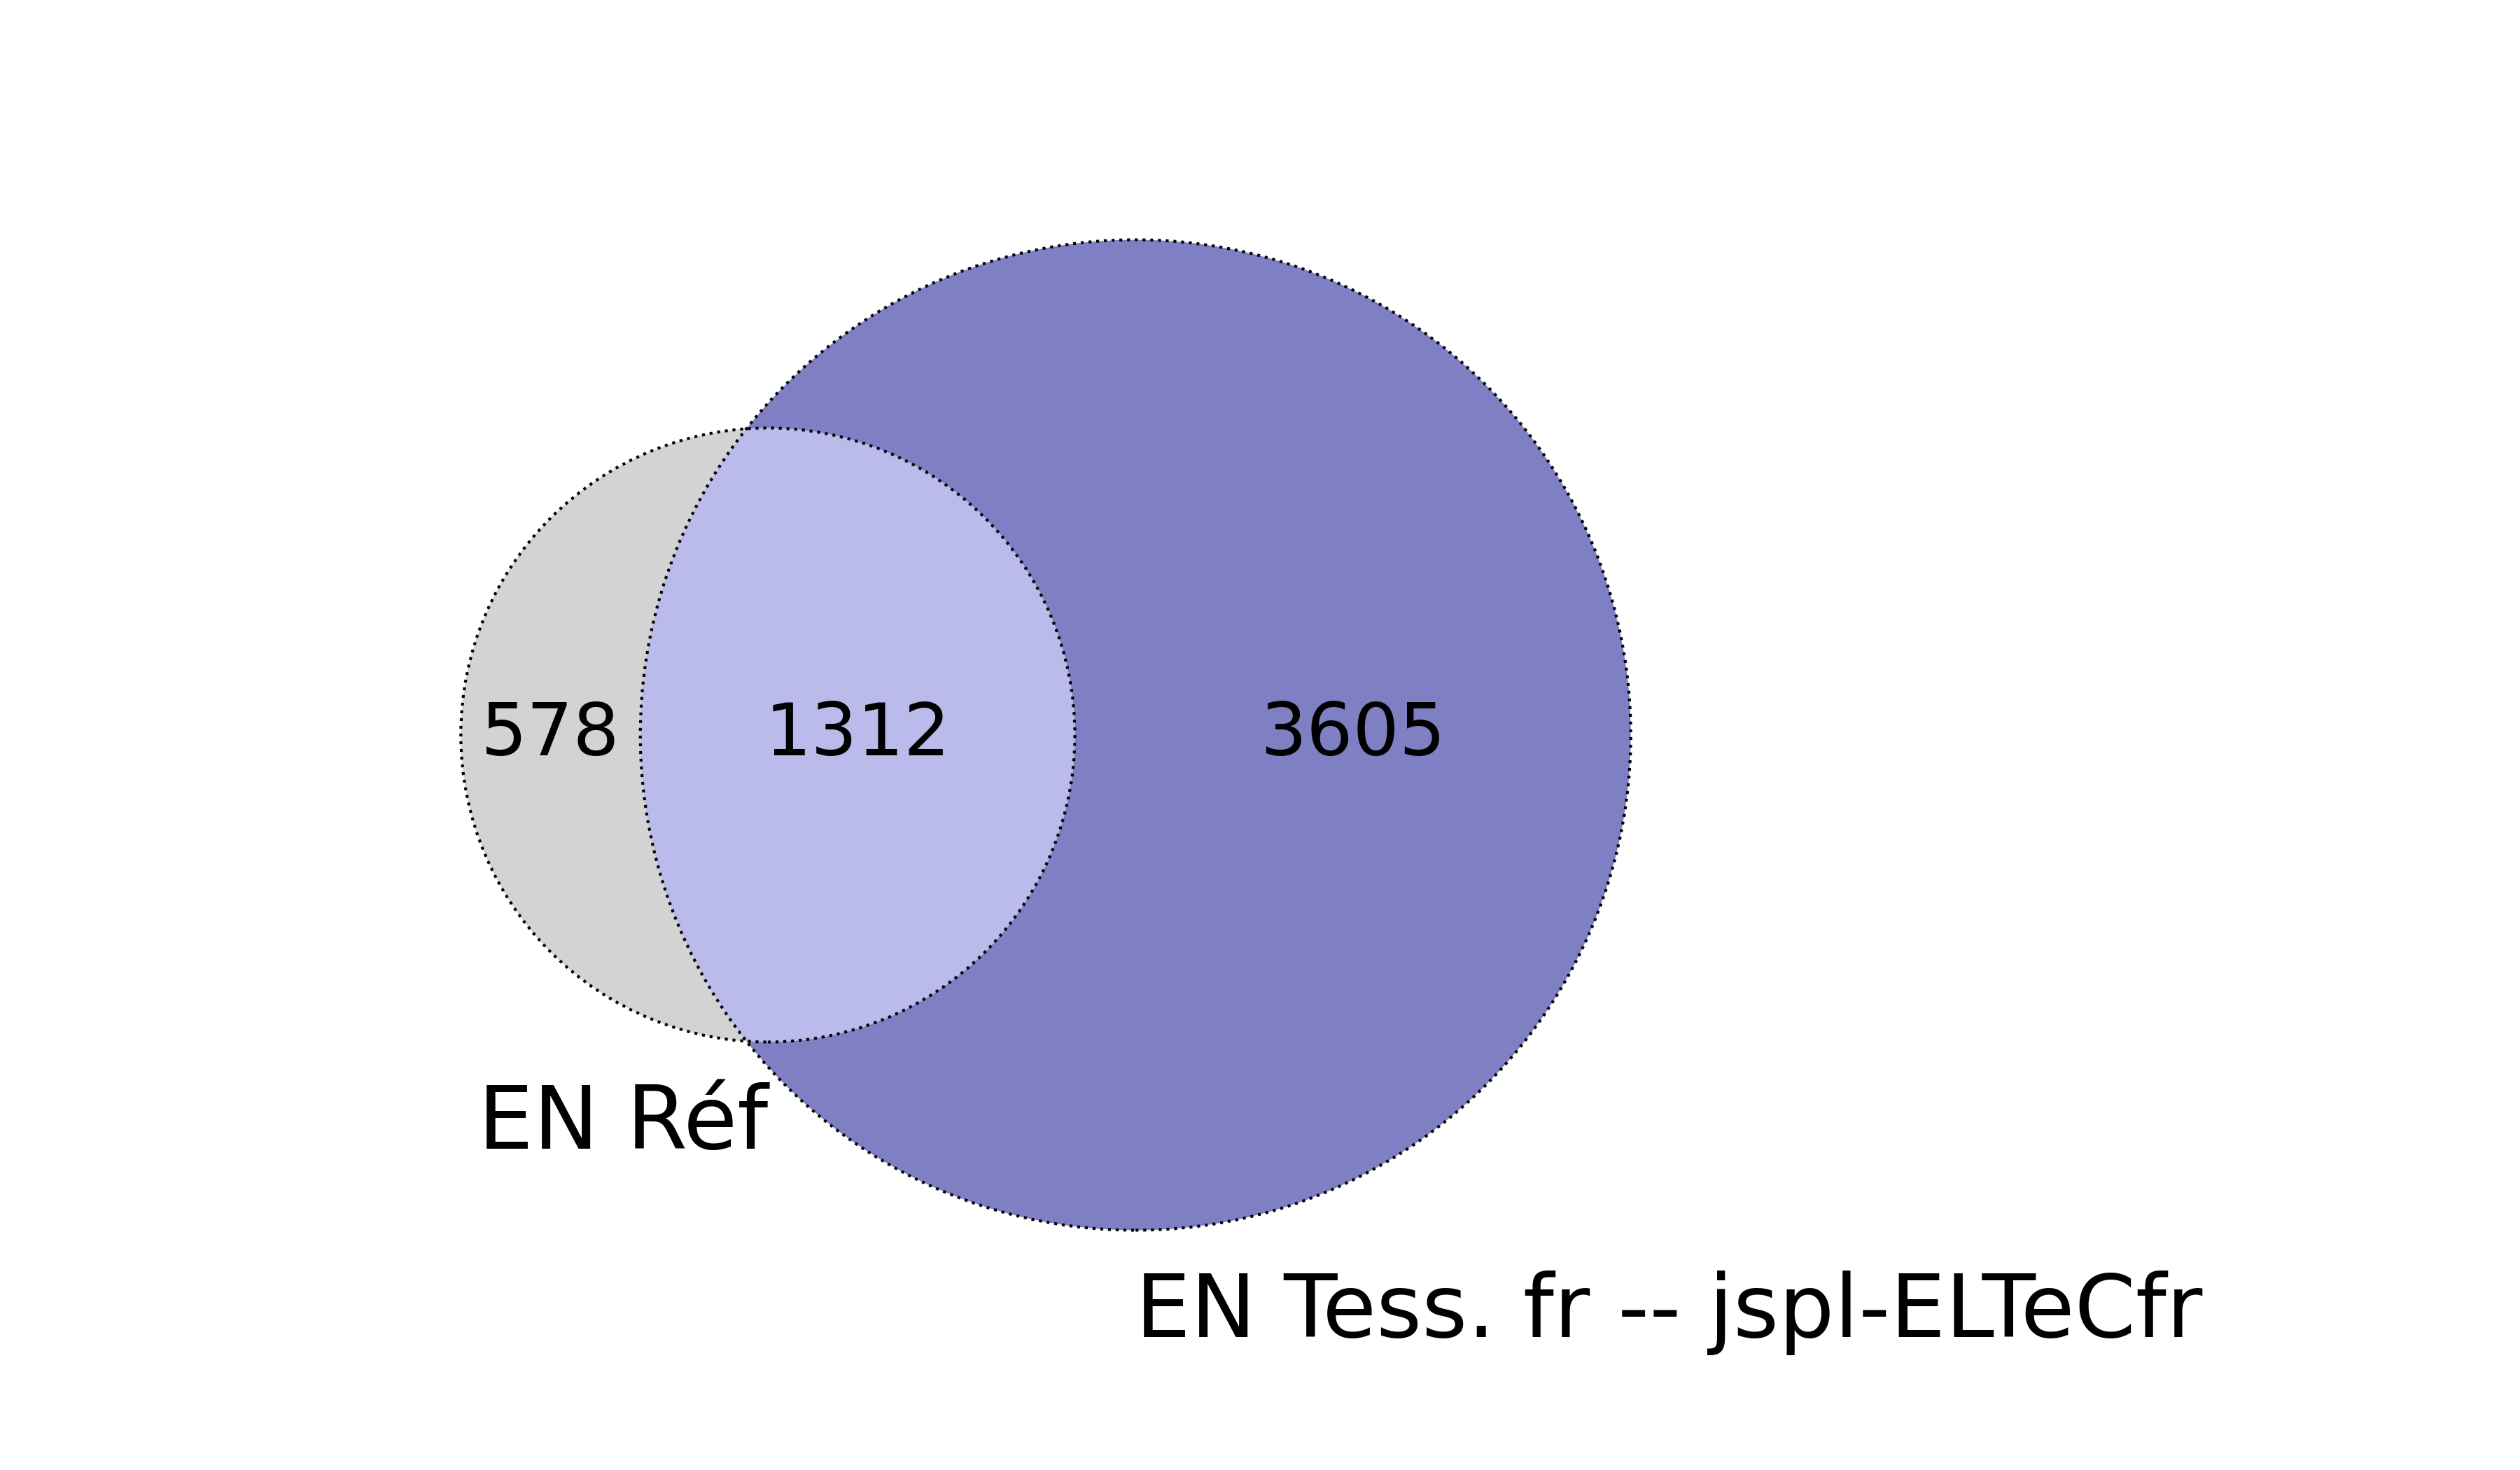
\includegraphics[width=1\textwidth]{IMAGES/INTERSECTIONS_GLOBALES/ELTeCFRA_Tess. fr -- jspl-ELTeCfr_spacy-lg-concat_intersection.png} % nouvelle figure ici avec Tess. fr. corrigé avec spaCy_lg
  \caption{Tess. fr. corrigé ELTeC-fr -- \texttt{spaCy\_lg}}
  \label{fig:ELTeCFRA_Tess -- jspl-ELTeCFR_spacy-lg-concat_intersection}
  \end{subfigure}
    \end{minipage}
%\caption{Intersections pour les configurations (\ref{fig:ELTeCFRA_Kraken -- jspl-fr_spacy-lg-concat_intersection.png
%}-\ref{fig:ELTeCFRA_Tess -- spacy-lg-concat_intersection}) Kraken-\texttt{spaCy\_lg} et Tess. fr.-\texttt{spaCy\_lg} non corrigées, et (\ref{fig:ELTeCFRA_Kraken -- jspl-ELTeCfr_spacy-lg-concat_intersection}-\ref{fig:ELTeCFRA_Tess -- jspl-ELTeCFR_spacy-lg-concat_intersection}) les configurations équivalentes corrigées avec JamSpell (modèle ELTeC), pour le sous-corpus ELTeC français.}
\caption{Intersections pour les configurations Kraken-\texttt{spaCy\_lg} et Tess. fr.-\texttt{spaCy\_lg} corrigées avec JamSpell pré-entraîné (\ref{fig:ELTeCFRA_Kraken -- jspl-fr_spacy-lg-concat_intersection.png}-\ref{fig:ELTeCFRA_Tess. fr -- jspl-fr_spacy-lg-concat_intersection.png}), et les configurations équivalentes corrigées avec JamSpell (modèle ELTeC), pour le sous-corpus ELTeC français (\ref{fig:ELTeCFRA_Kraken -- jspl-ELTeCfr_spacy-lg-concat_intersection}-\ref{fig:ELTeCFRA_Tess -- jspl-ELTeCFR_spacy-lg-concat_intersection}).}
\label{fig:intersection_globale-kraken}
\end{figure}

Ce fait peut être lu à l'aune des observations présentées dans le tableau \ref{tab:typologie_erreurs-corr_ELTeCEng} rapportant la typologie des erreurs de corrections. Autrement dit, la correction automatique ne transforme pas toutes les EN contaminées par la ROC en EN corrigées strictement associables avec les EN du groupe de référence. Ainsi les BOIC (``Morlincourt'' qui devient ``Martincourt''), se cumulant aux EN contaminées MOI (``Morlincourtl'' qui reste ``Morlincourtl''), rendent les résultats des intersections moins bons. Il semble qu'en moyenne pour les corpus ELTeC français, anglais et portugais et celui de la TGB la correction automatique avec le modèle entraîné sur une partie de chaque sous-corpus ELTeC fasse perdre 5\% des EN dans l'intersection avec Kraken et 10\% avec Tesseract, alors que concernant les modèles pré-entraînés on perd 3\% avec Kraken et 9\% avec Tesseract. Cette expérience est l'occasion de démontrer les limites d'une évaluation stricte de la REN sur des textes bruités et leurs versions corrigées. Il est notable que les contaminations de ROC d'une part et de la correction automatique d'autre part ne sont pas véritablement un frein à la REN, mais l'évaluation automatique des résultats n'est pas triviale.

%%%%%%%%%%%%%%%% Ancienne figure avec les intersections pour la config Tess-spaCy_lg corrigées avec le modèle pré-entraîné de JamSpell et le modèle ELTeC, pour le sous-corpus ELTeC fr %%%%%%%%%%%%%%%%%%

%\begin{figure}[h!]
%%    \begin{minipage}{7cm}
%%  \begin{subfigure}{1\textwidth}
%%  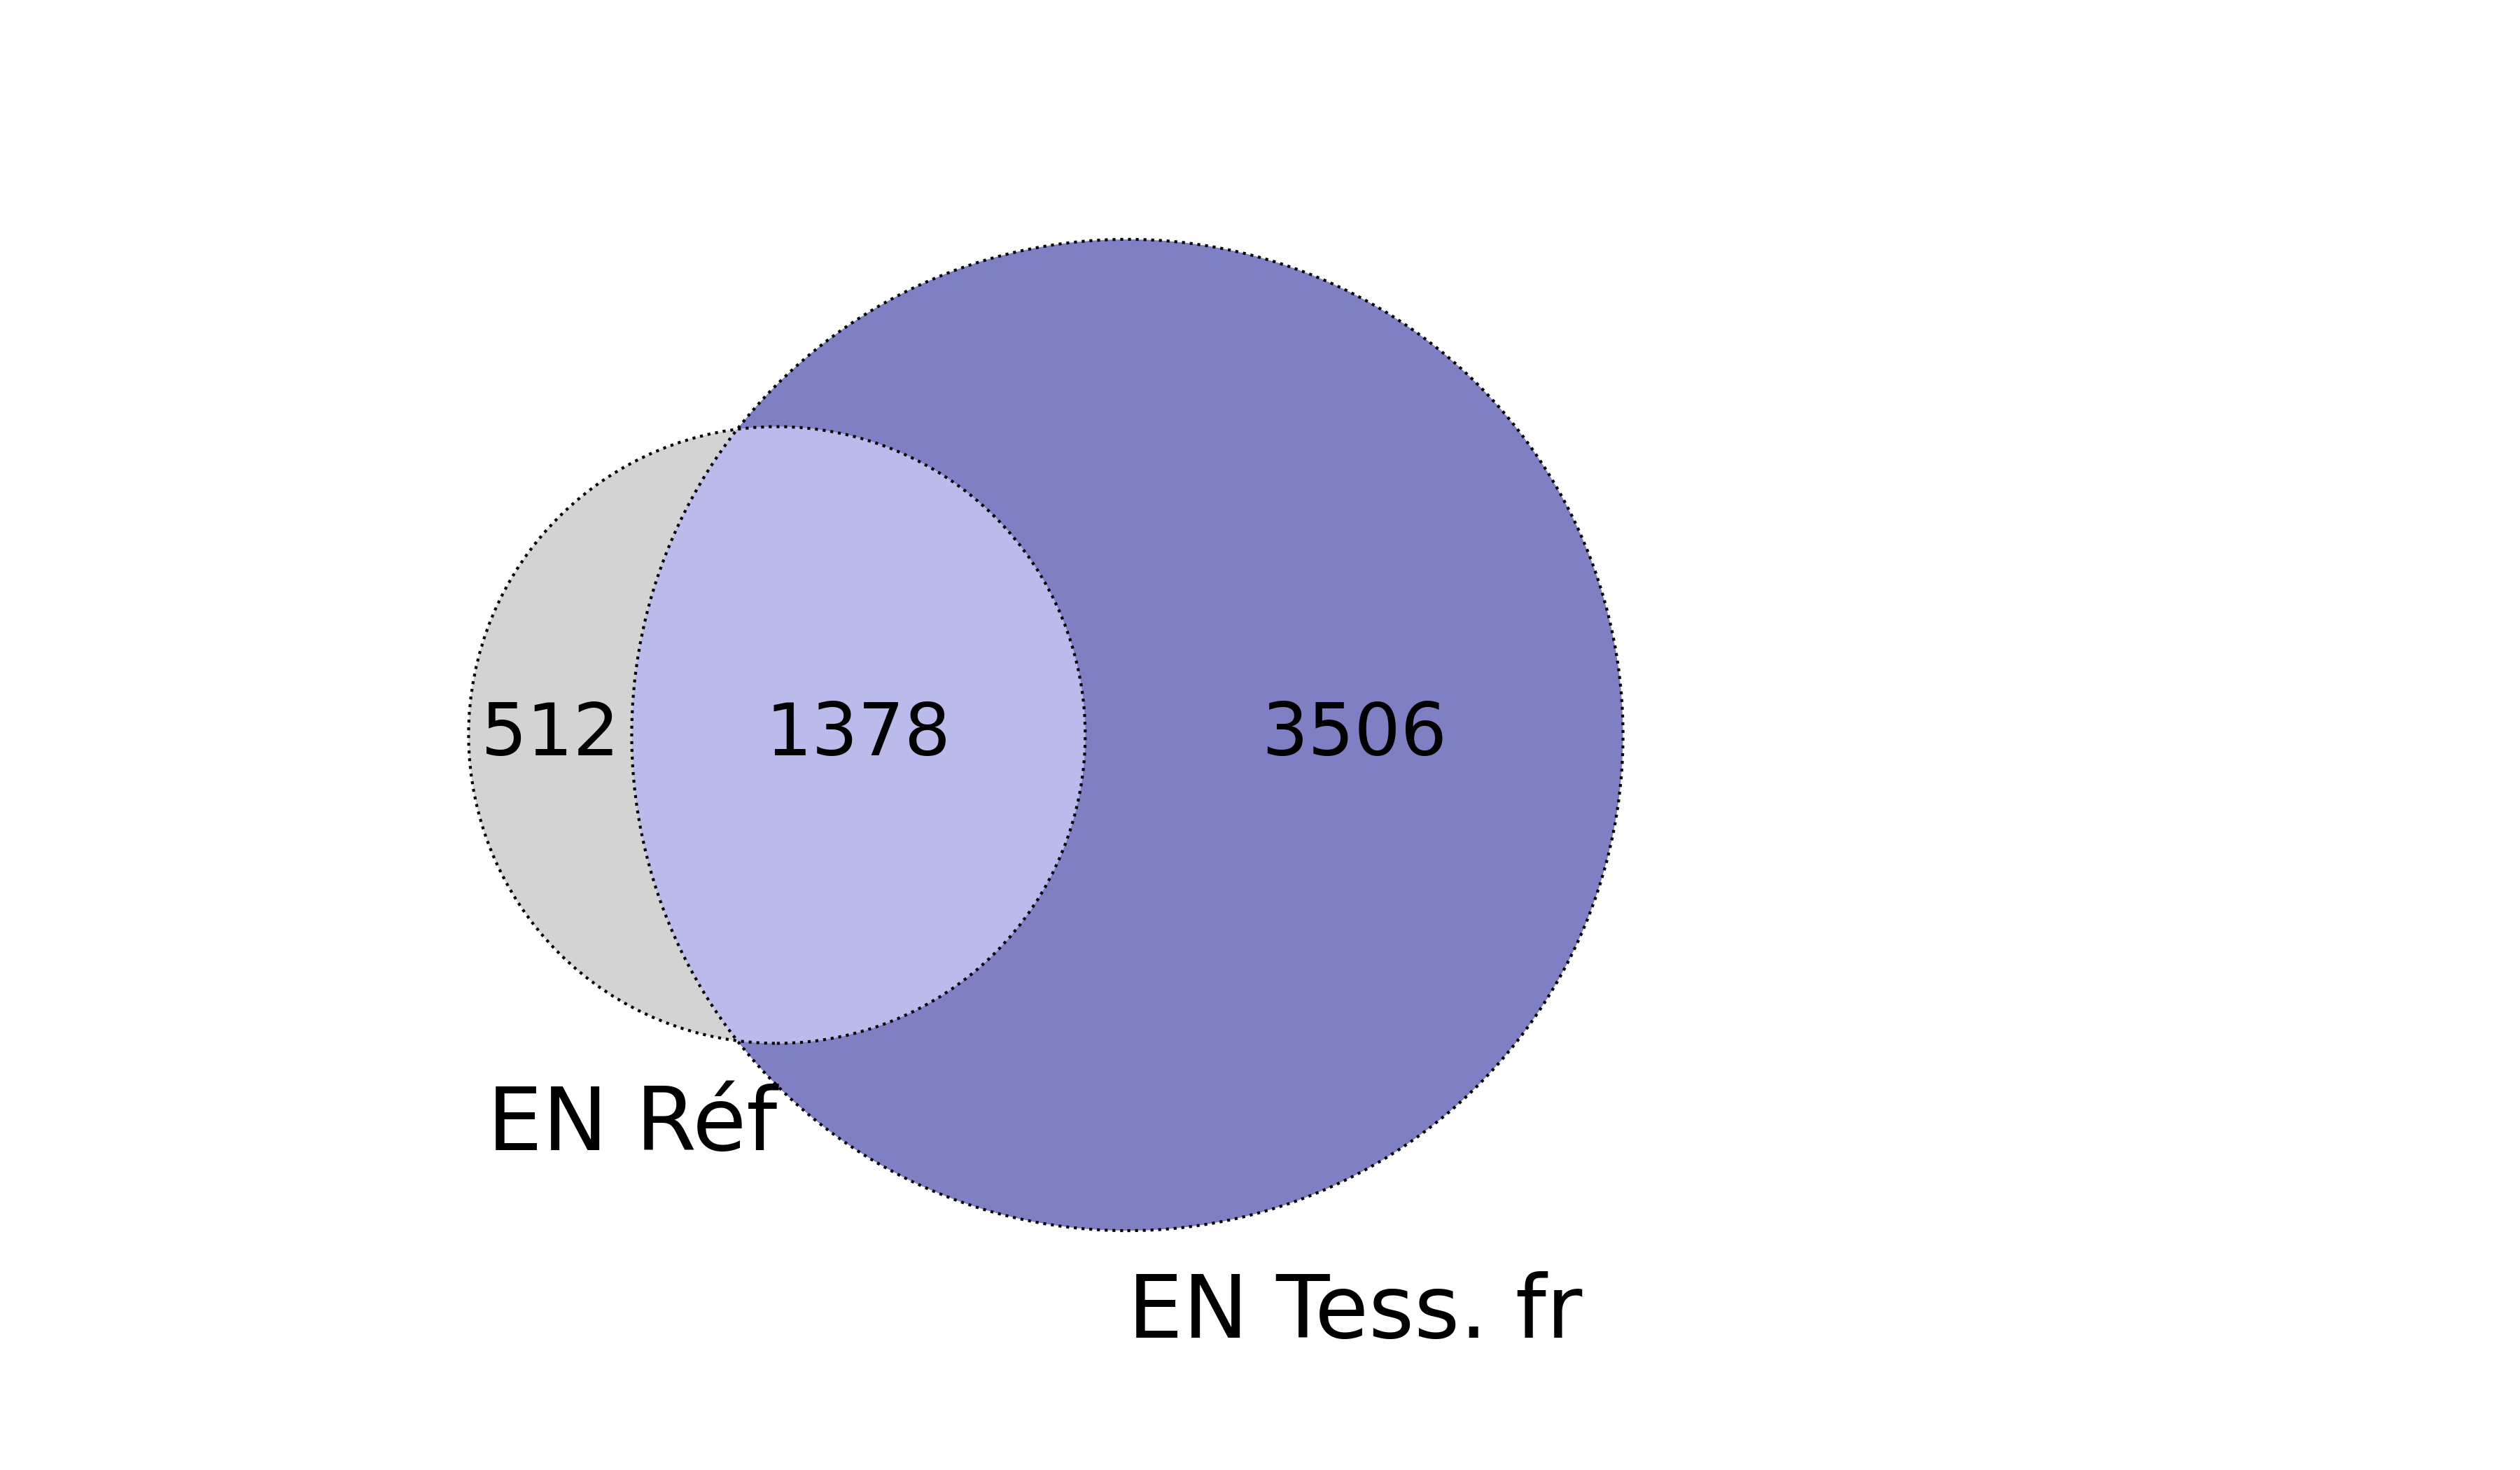
\includegraphics[width=1\textwidth]{IMAGES/INTERSECTIONS_GLOBALES/ELTeCFRA_Tess. fr_spacy-lg-concat_intersection.png} 
%%  \caption{Tess. fr. --\texttt{spaCy\_lg}}
%%  \label{fig:ELTeCFRA_Tess. fr_spacy-lg-concat_intersection}
%%  \end{subfigure}
%%  \end{minipage}
%%  \begin{minipage}{7cm}
%%  \begin{subfigure}{1\textwidth}
%%  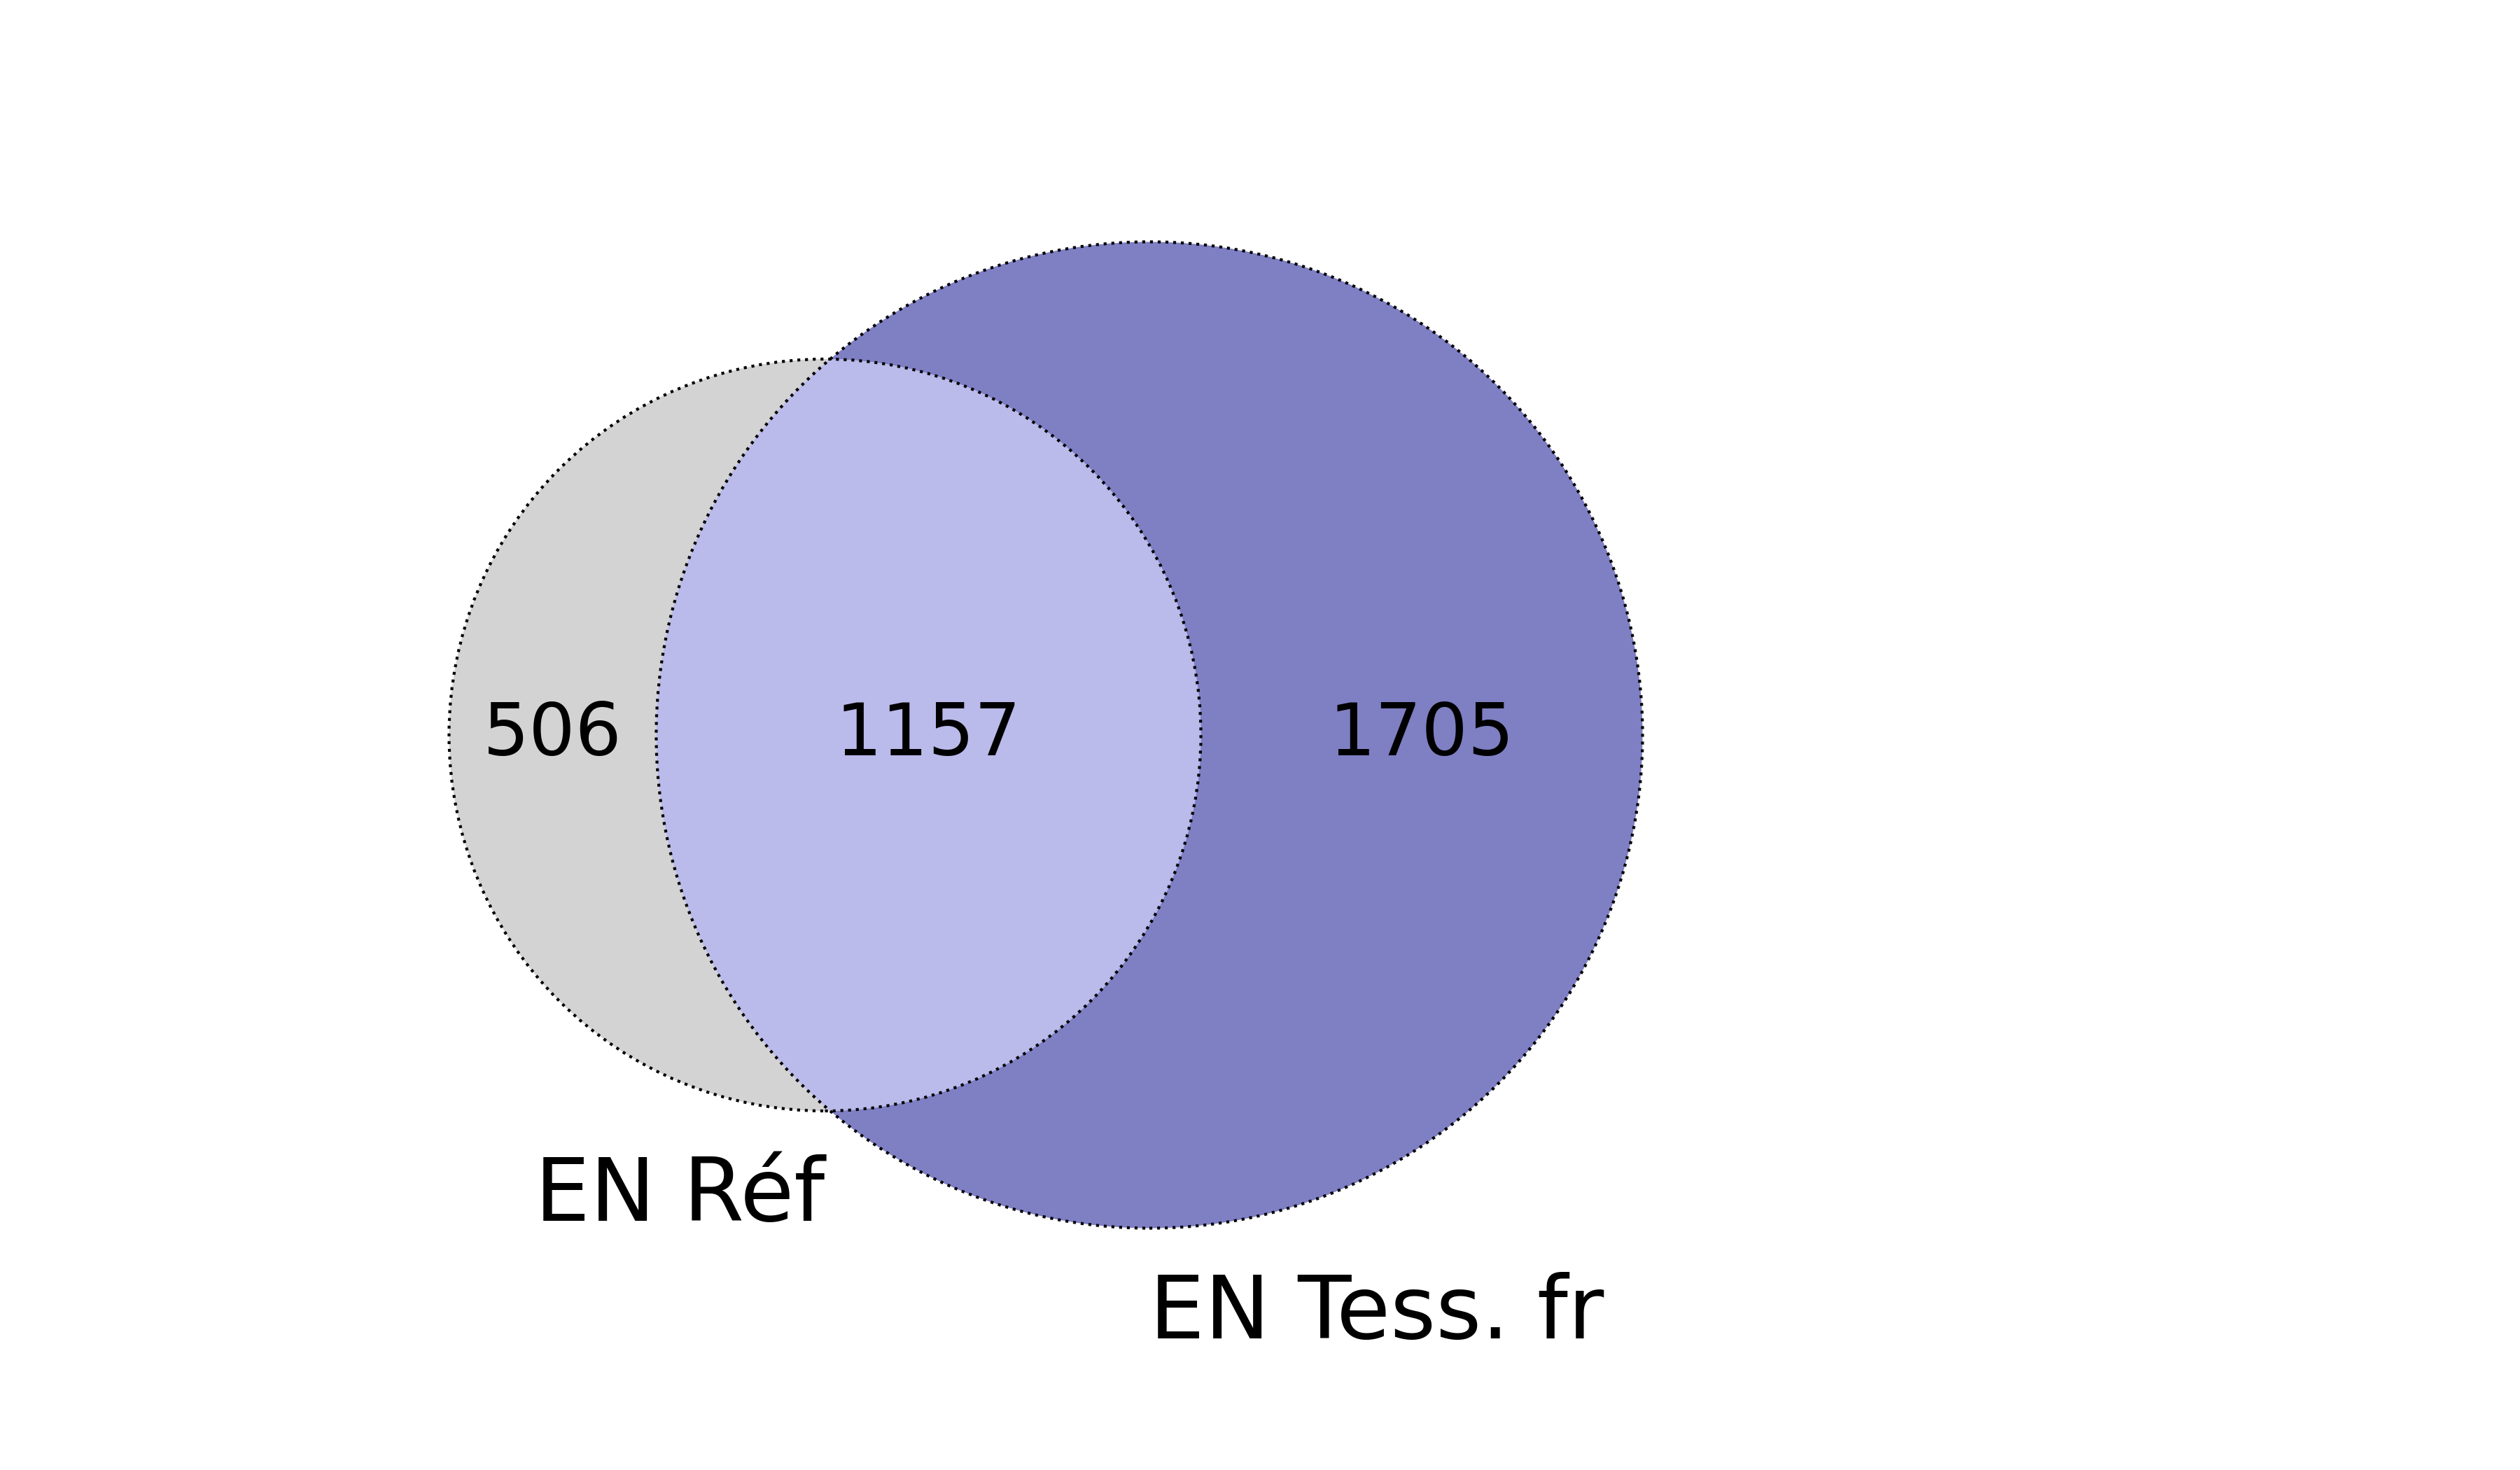
\includegraphics[width=1\textwidth]{IMAGES/INTERSECTIONS_GLOBALES/ELTeCFRA_Tess. fr_stanza-concat_intersection.png}
%%  \caption{Tess. fr. -- \texttt{stanza}}
%% % \label{fig:ELTeCFRA_Tess. fr_stanza-concat_intersection}
%%  \end{subfigure}
%%    \end{minipage}
%%\begin{minipage}{7cm}
%%  \begin{subfigure}{1\textwidth}
%%  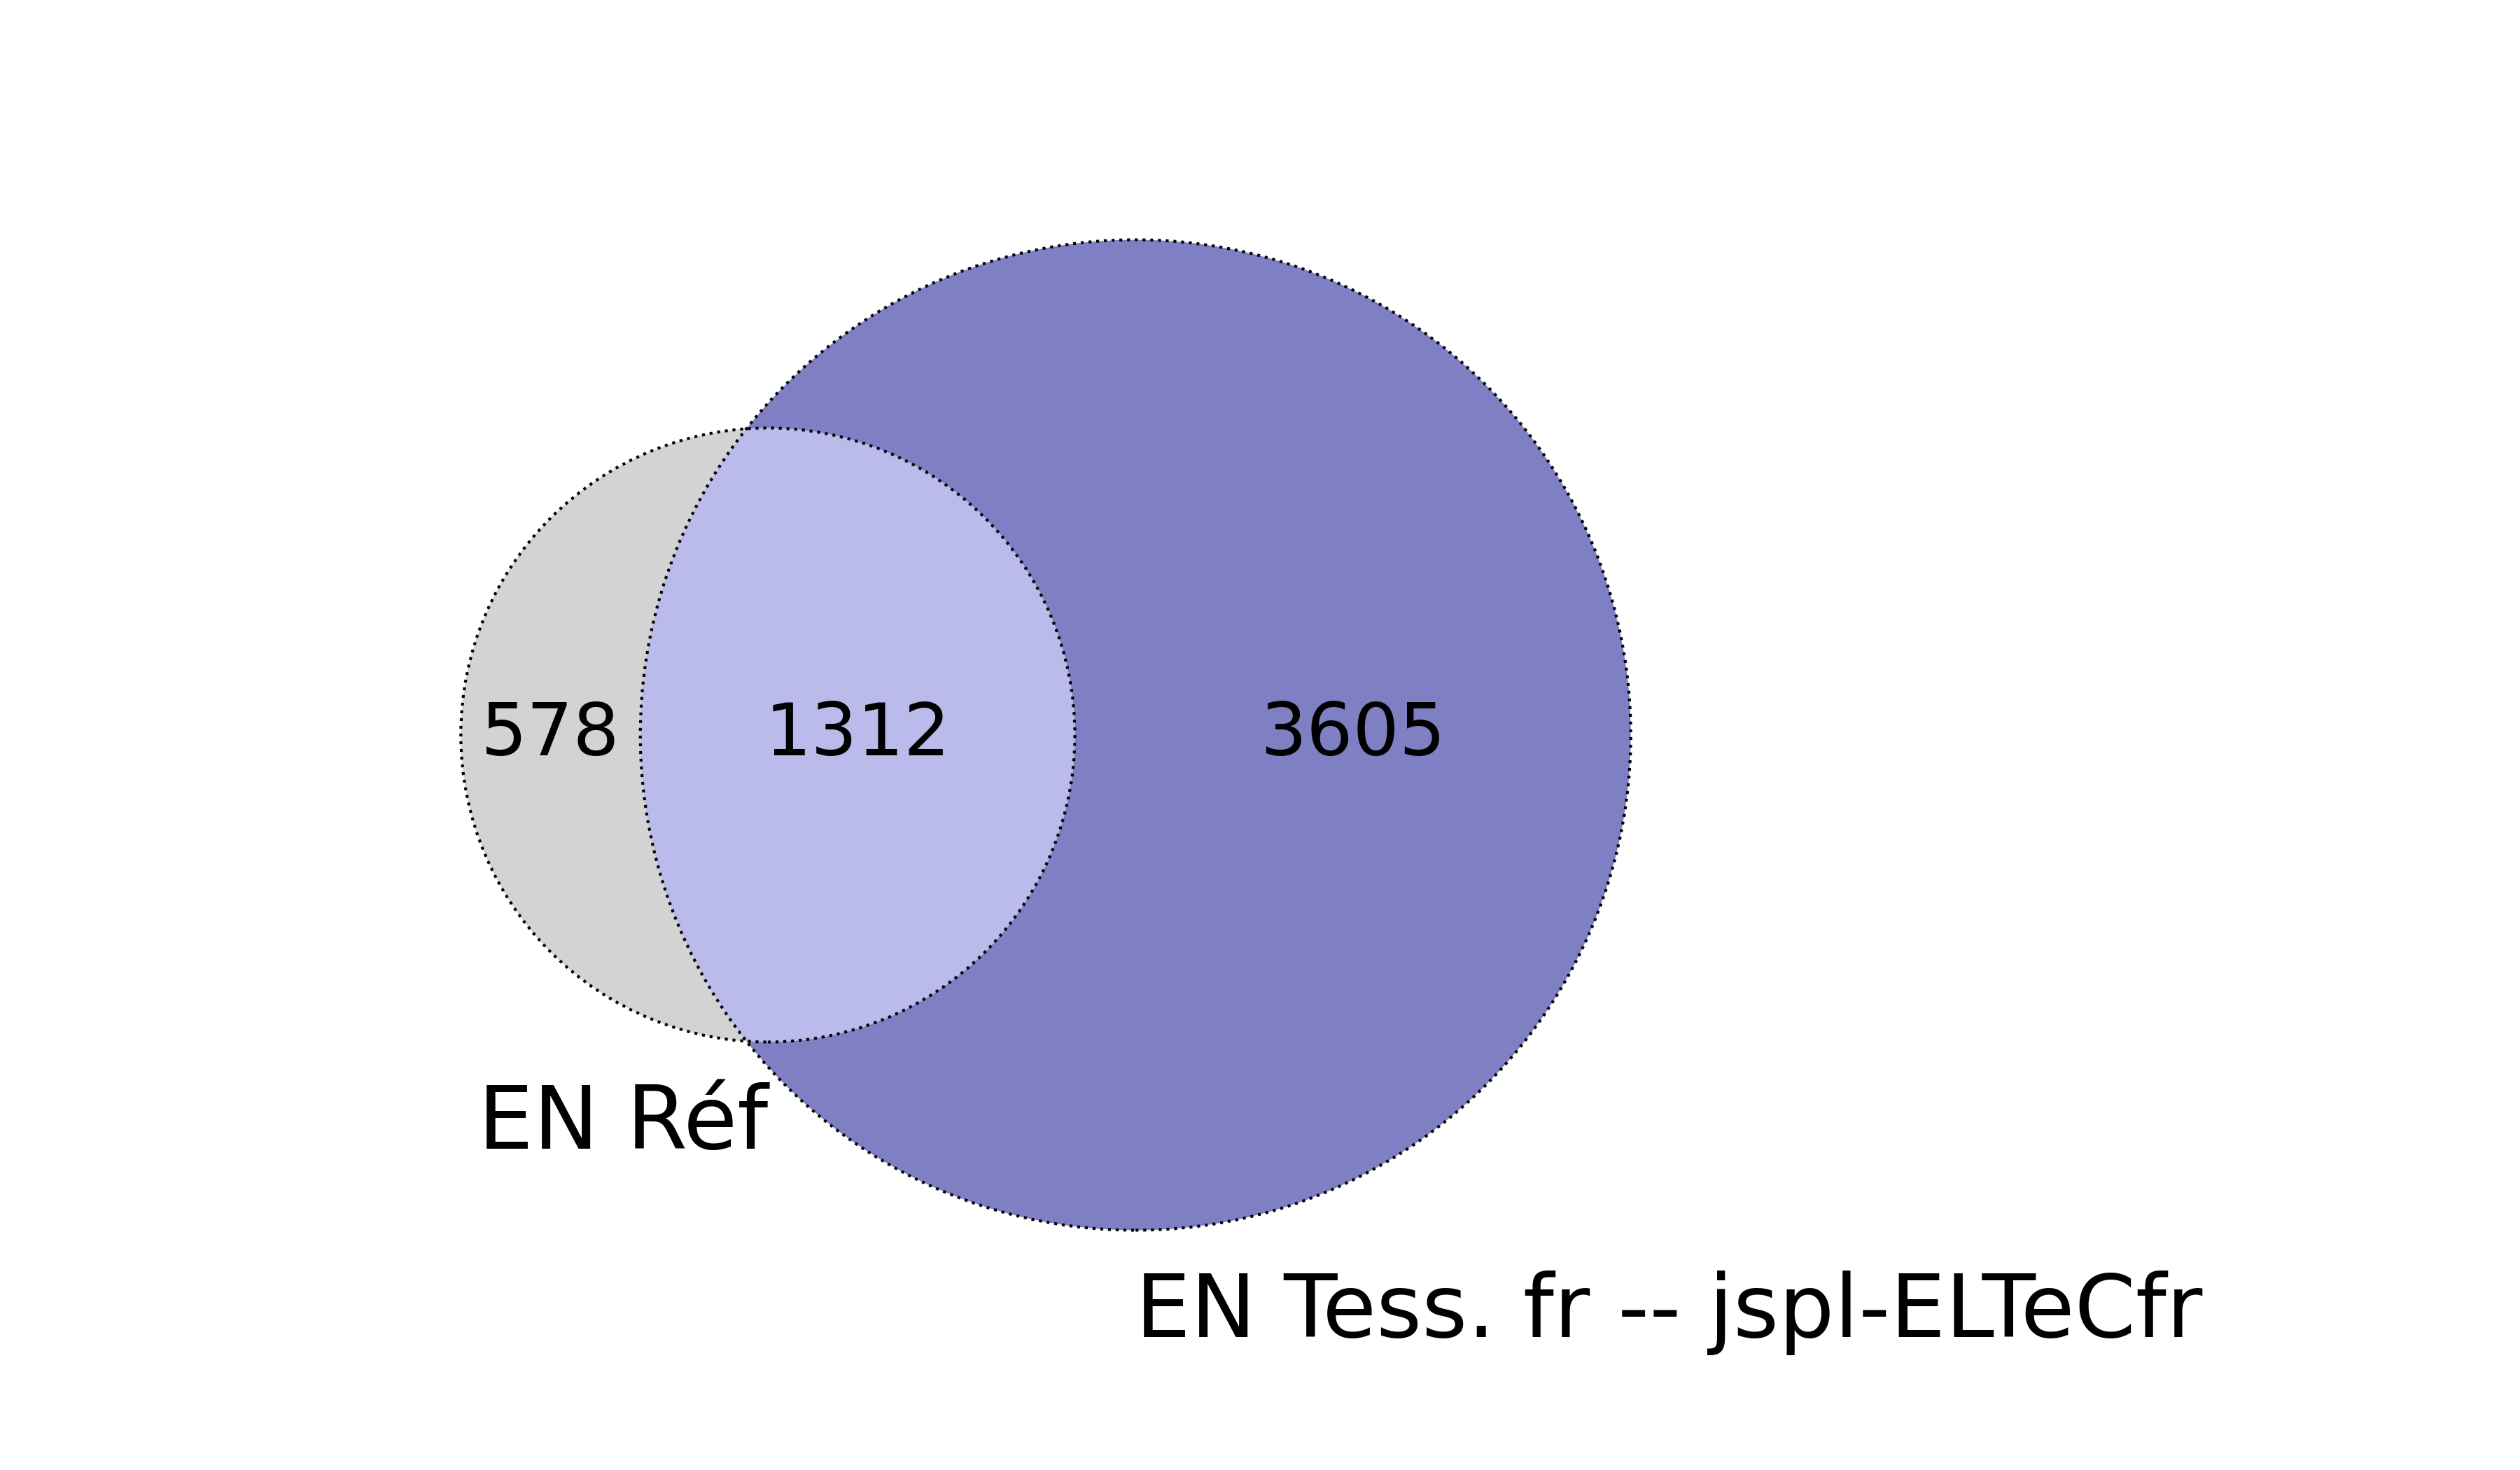
\includegraphics[width=1\textwidth]{IMAGES/INTERSECTIONS_GLOBALES/ELTeCFRA_Tess. fr -- jspl-ELTeCfr_spacy-lg-concat_intersection.png} 
%%  \caption{Tess. fr. corrigé -- \texttt{spaCy\_lg}}
%%  \label{fig:ELTeCFRA_Tess. fr -- jspl-ELTeCfr_spacy-lg-concat_intersection}
%%  \end{subfigure}
%%  \end{minipage}
%  \begin{minipage}{7cm}
%  \begin{subfigure}{1\textwidth}
%  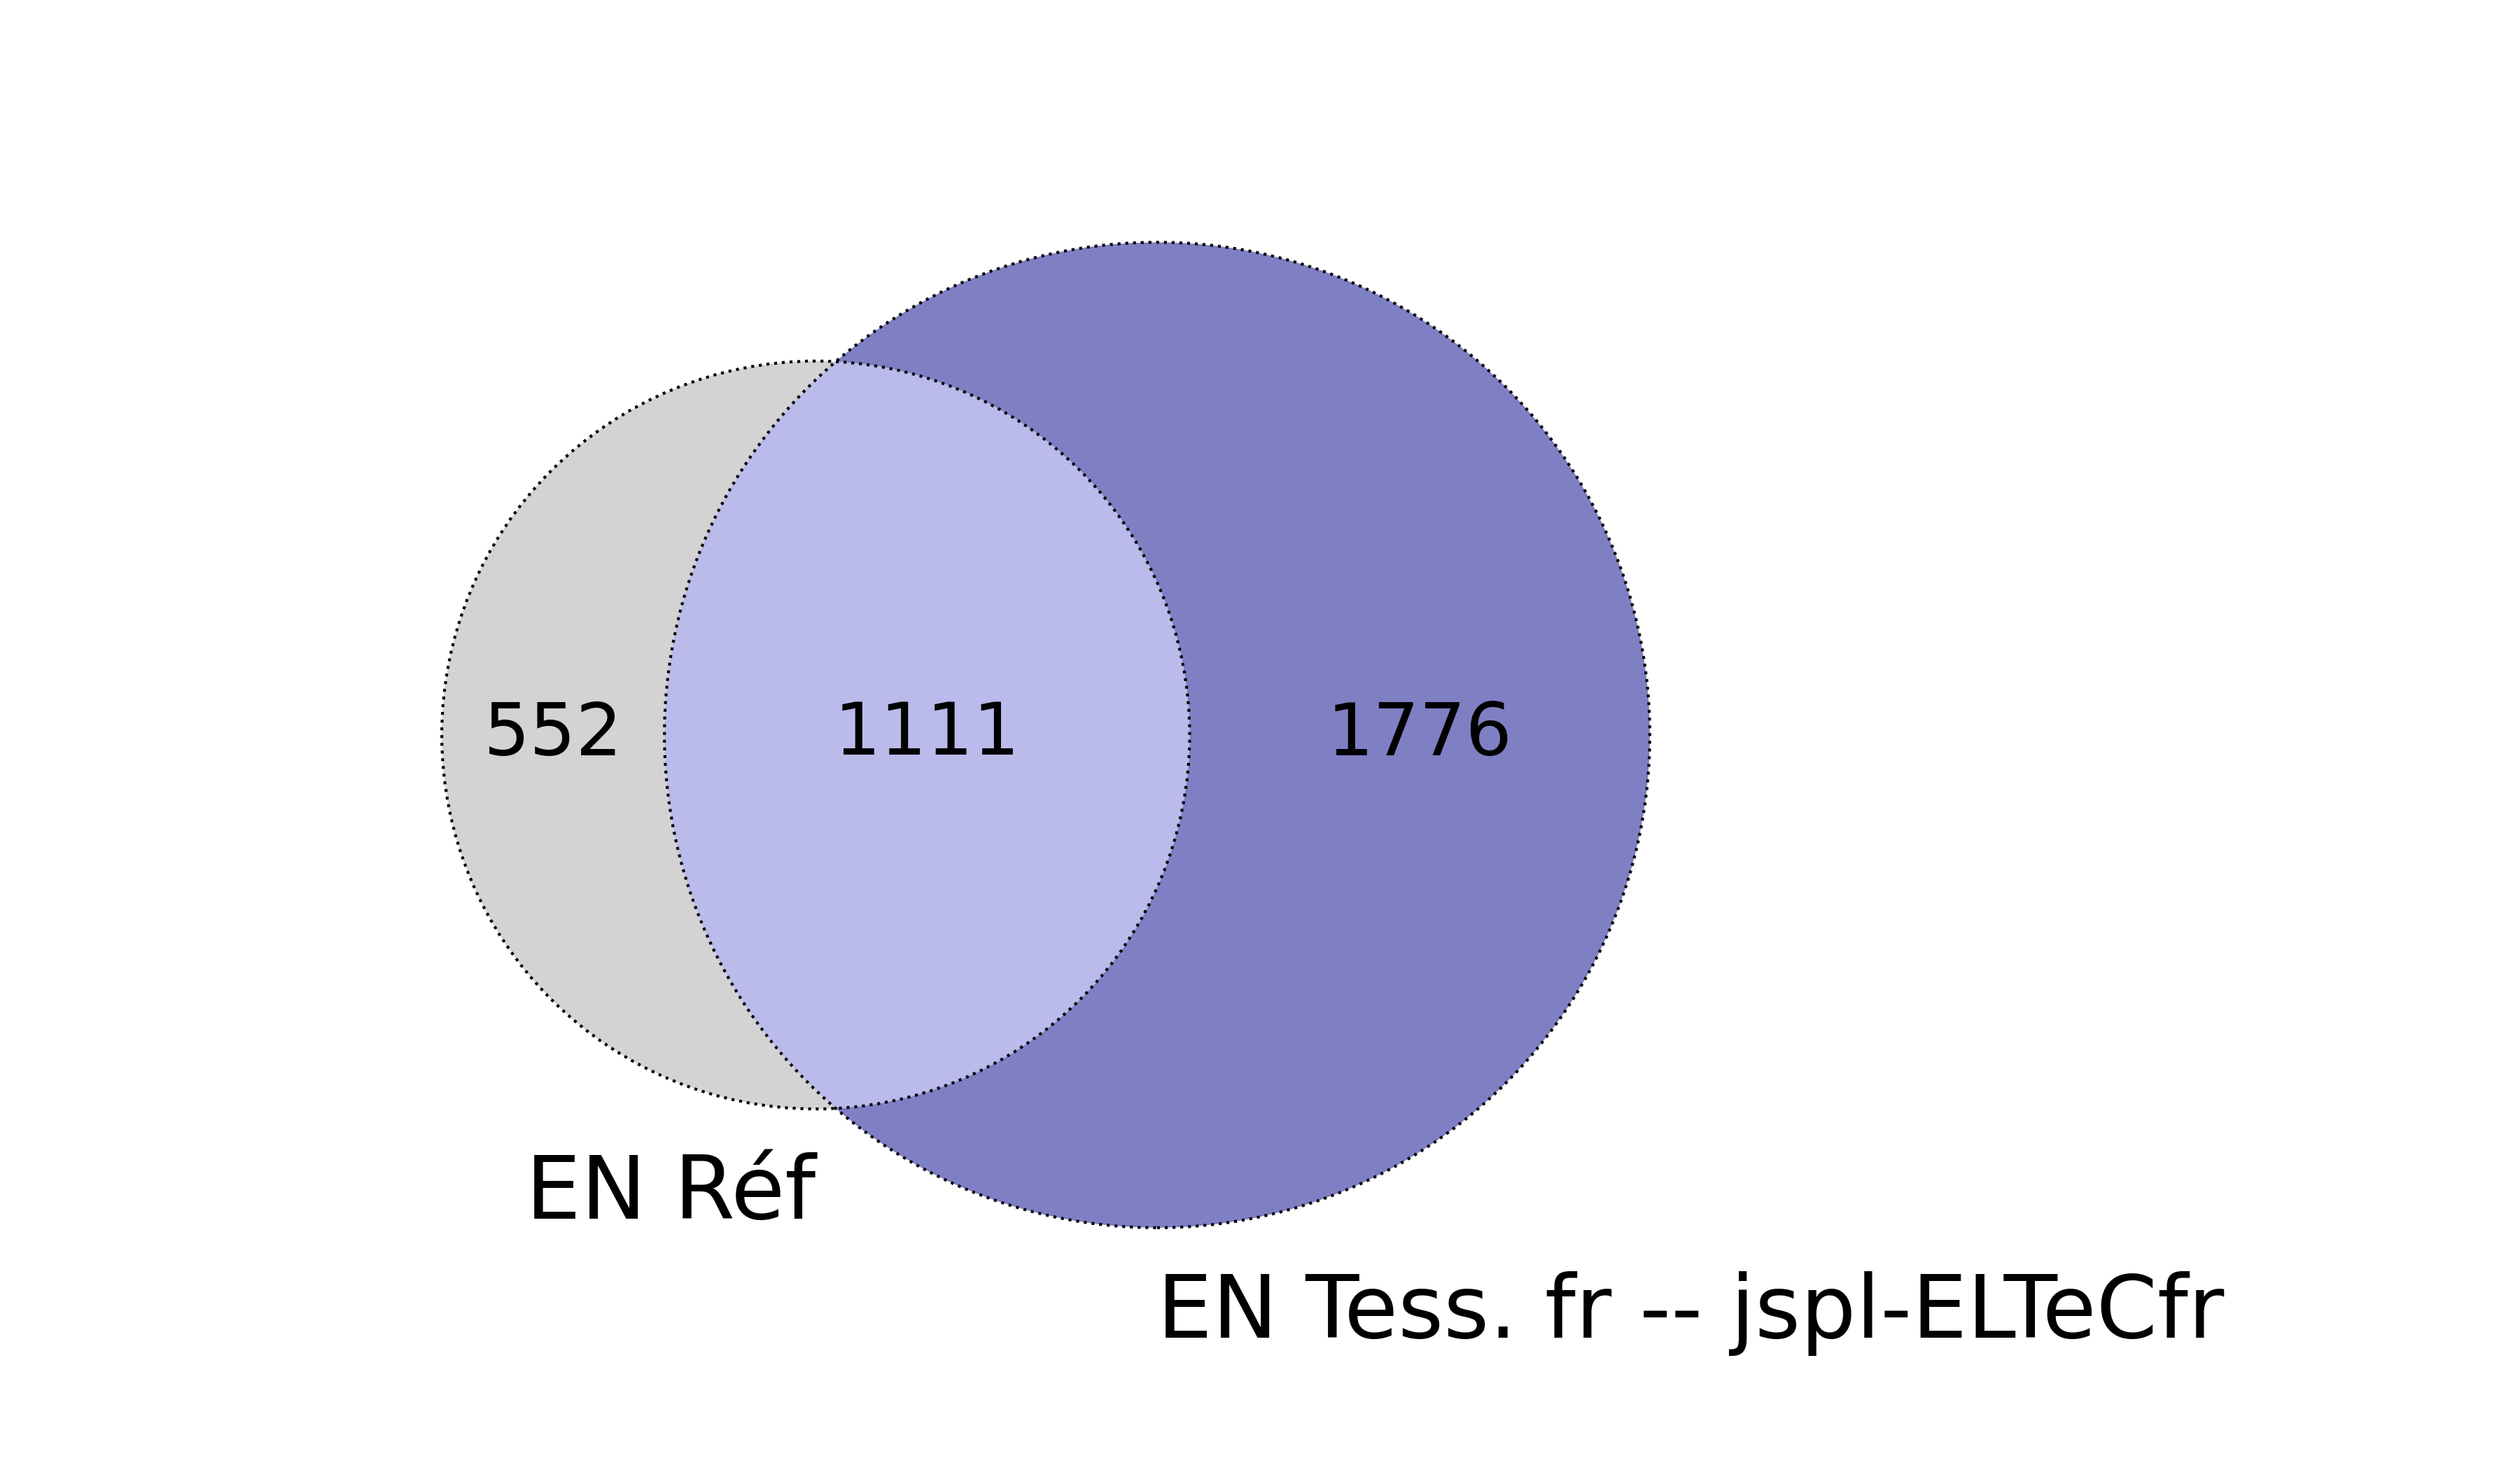
\includegraphics[width=1\textwidth]{IMAGES/INTERSECTIONS_GLOBALES/ELTeCFRA_Tess. fr -- jspl-ELTeCfr_stanza-concat_intersection.png}
%  \caption{Tess. fr. corrigé -- \texttt{stanza}}
%  \label{fig:ELTeCFRA_Tess. fr -- jspl-ELTeCfr_stanza-concat_intersection}
%  \end{subfigure}
%    \end{minipage}
%\begin{minipage}{7cm}
%  \begin{subfigure}{1\textwidth}
%  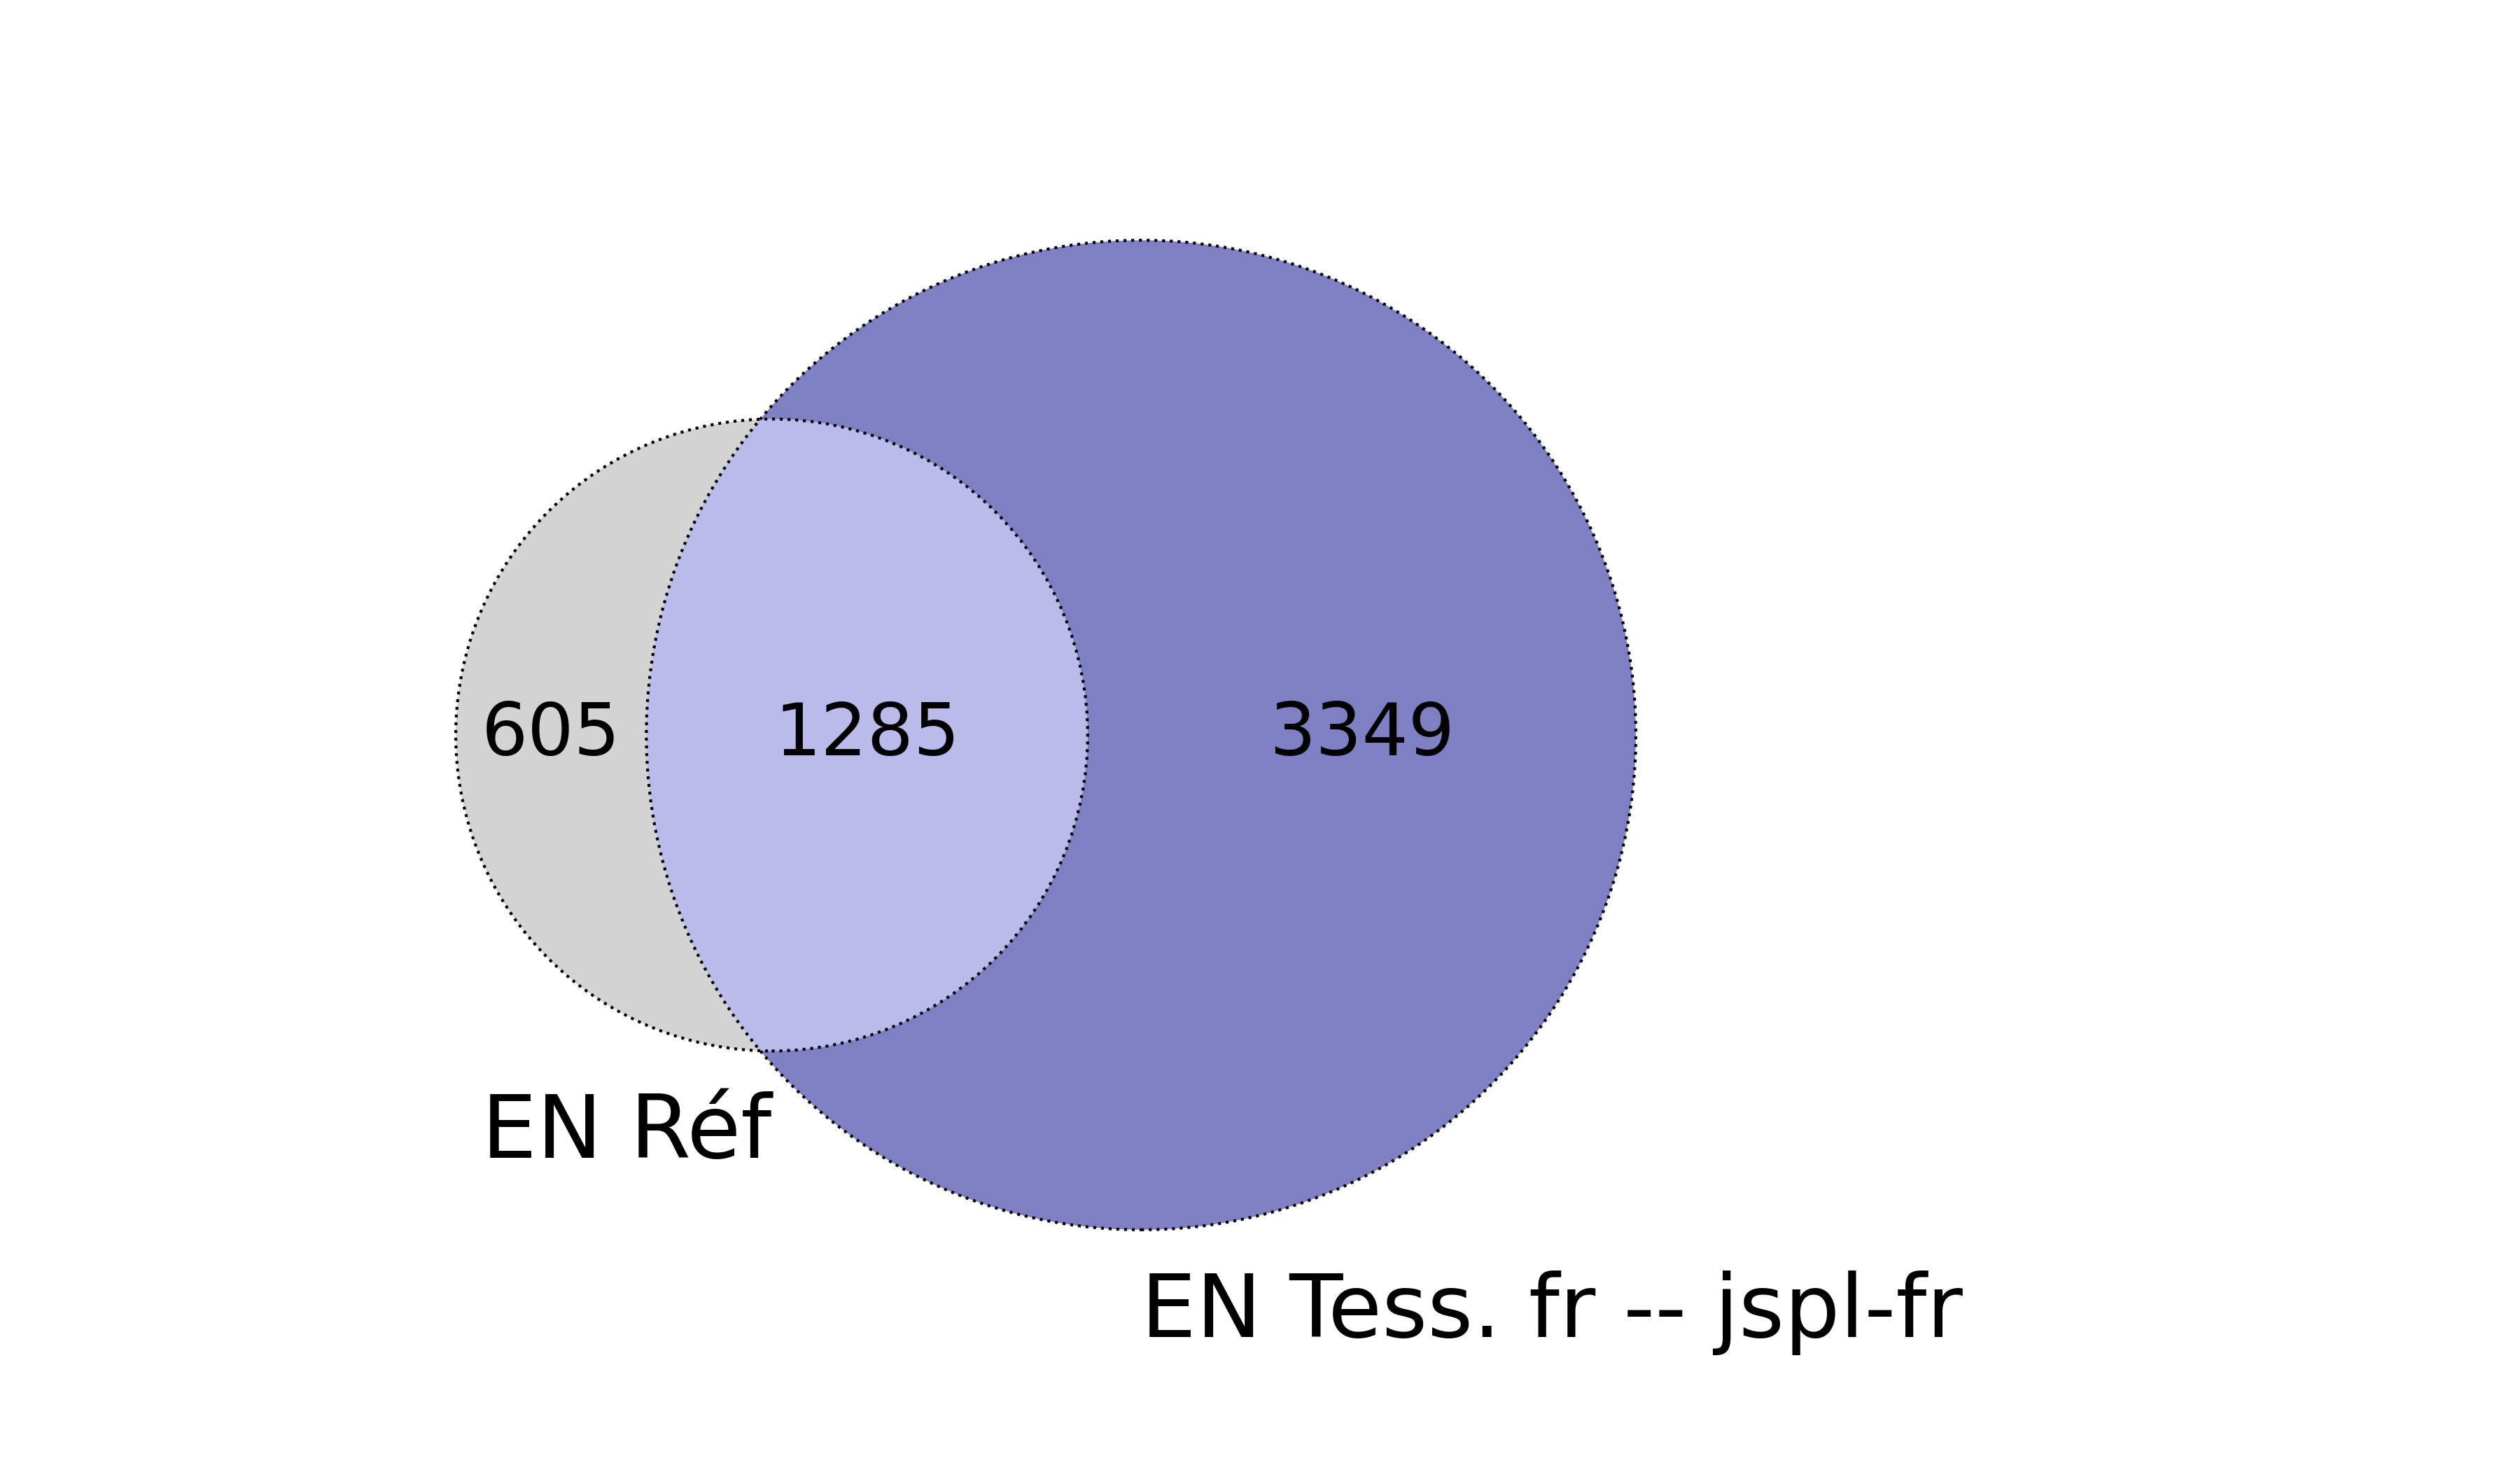
\includegraphics[width=1\textwidth]{IMAGES/INTERSECTIONS_GLOBALES/ELTeCFRA_Tess. fr -- jspl-fr_spacy-lg-concat_intersection.png} 
%  \caption{Tess. fr. corrigé -- \texttt{spaCy\_lg}}
%  \label{fig:ELTeCFRA_Tess. fr -- jspl-fr_spacy-lg-concat_intersection}
%  \end{subfigure}
%  \end{minipage}
%  \begin{minipage}{7cm}
%  \begin{subfigure}{1\textwidth}
%  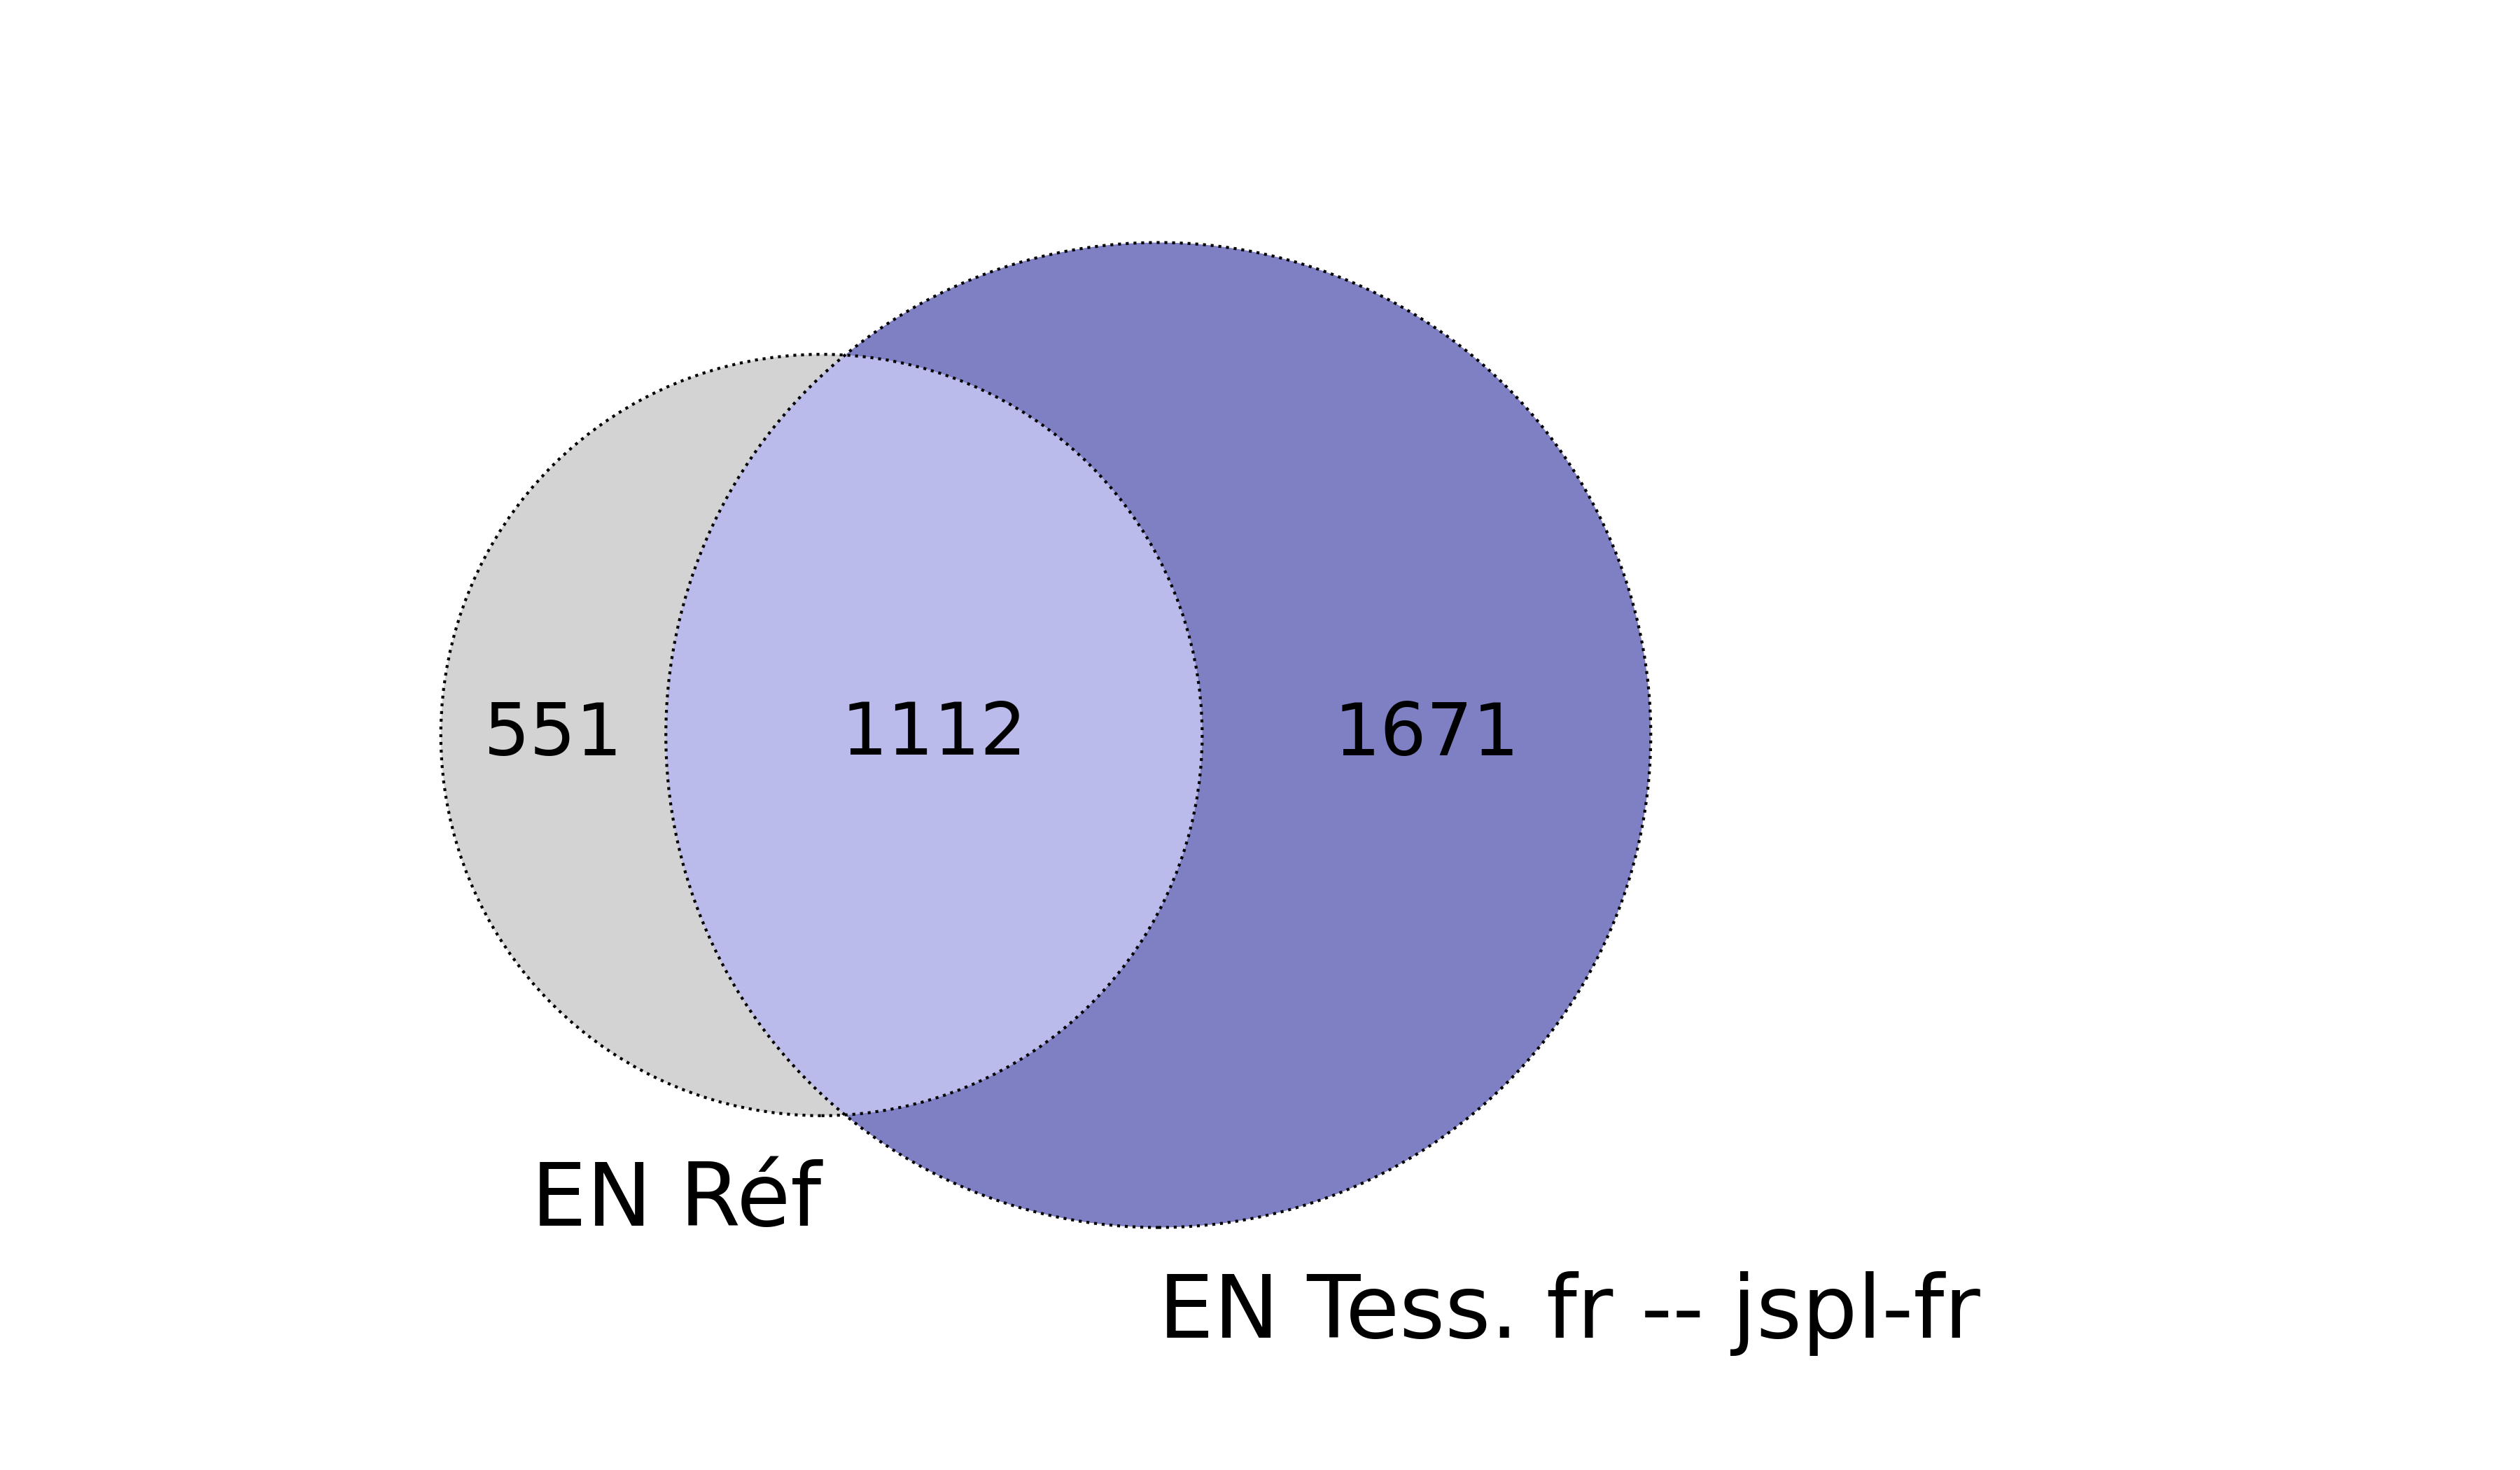
\includegraphics[width=1\textwidth]{IMAGES/INTERSECTIONS_GLOBALES/ELTeCFRA_Tess. fr -- jspl-fr_stanza-concat_intersection.png}
%  \caption{Tess. fr. corrigé -- \texttt{stanza}}
%  \label{fig:ELTeCFRA_Tess. fr -- jspl-fr_stanza-concat_intersection}
%  \end{subfigure}
%    \end{minipage}
%\caption{Intersections pour la configuration Tess-\texttt{spaCy\_lg} corrigées avec le modèle pré-entrainer de JamSpell et le modèle ELTeC, pour le sous-corpus ELTeC français.}
%\label{fig:intersection-globale-tess}
%\end{figure}
\subsection{Comment dépasser les problèmes d'alignements ? }
\label{subsec:ditances_creux_COR-OCR-IMPACT-NER}
\subsubsection{Mesures de distance textuelle}

Dans le but d'approfondir nos évaluation et de dépasser les verrous de l'évaluation stricte, nous employons des mesures de distance textuelle afin de rendre plus souple nos critères d'évaluation des résultats de REN sur les sorties de ROC bruitées et leurs corrections automatiques. Nous avons privilégié les métriques de Jaccard et cosinus car elles sont considérées comme des mesures de référence quand il est question de (dis)similarité textuelle \cite{buscaldi2020calcul}. Les sous-figures \ref{fig:ELTeC-Por_REF_jaccard}-\ref{fig:ELTeC-Por_REF_cosinus} illustrent les résultats obtenus pour les textes de référence et les différentes versions de ROC pour le corpus ELTeC portugais avec les mesures de jaccard et cosinus, et les résultats pour les autres corpus de notre études sont similaires.

\begin{figure}[h!]
   \centering
      \begin{subfigure}{0.45\textwidth}
  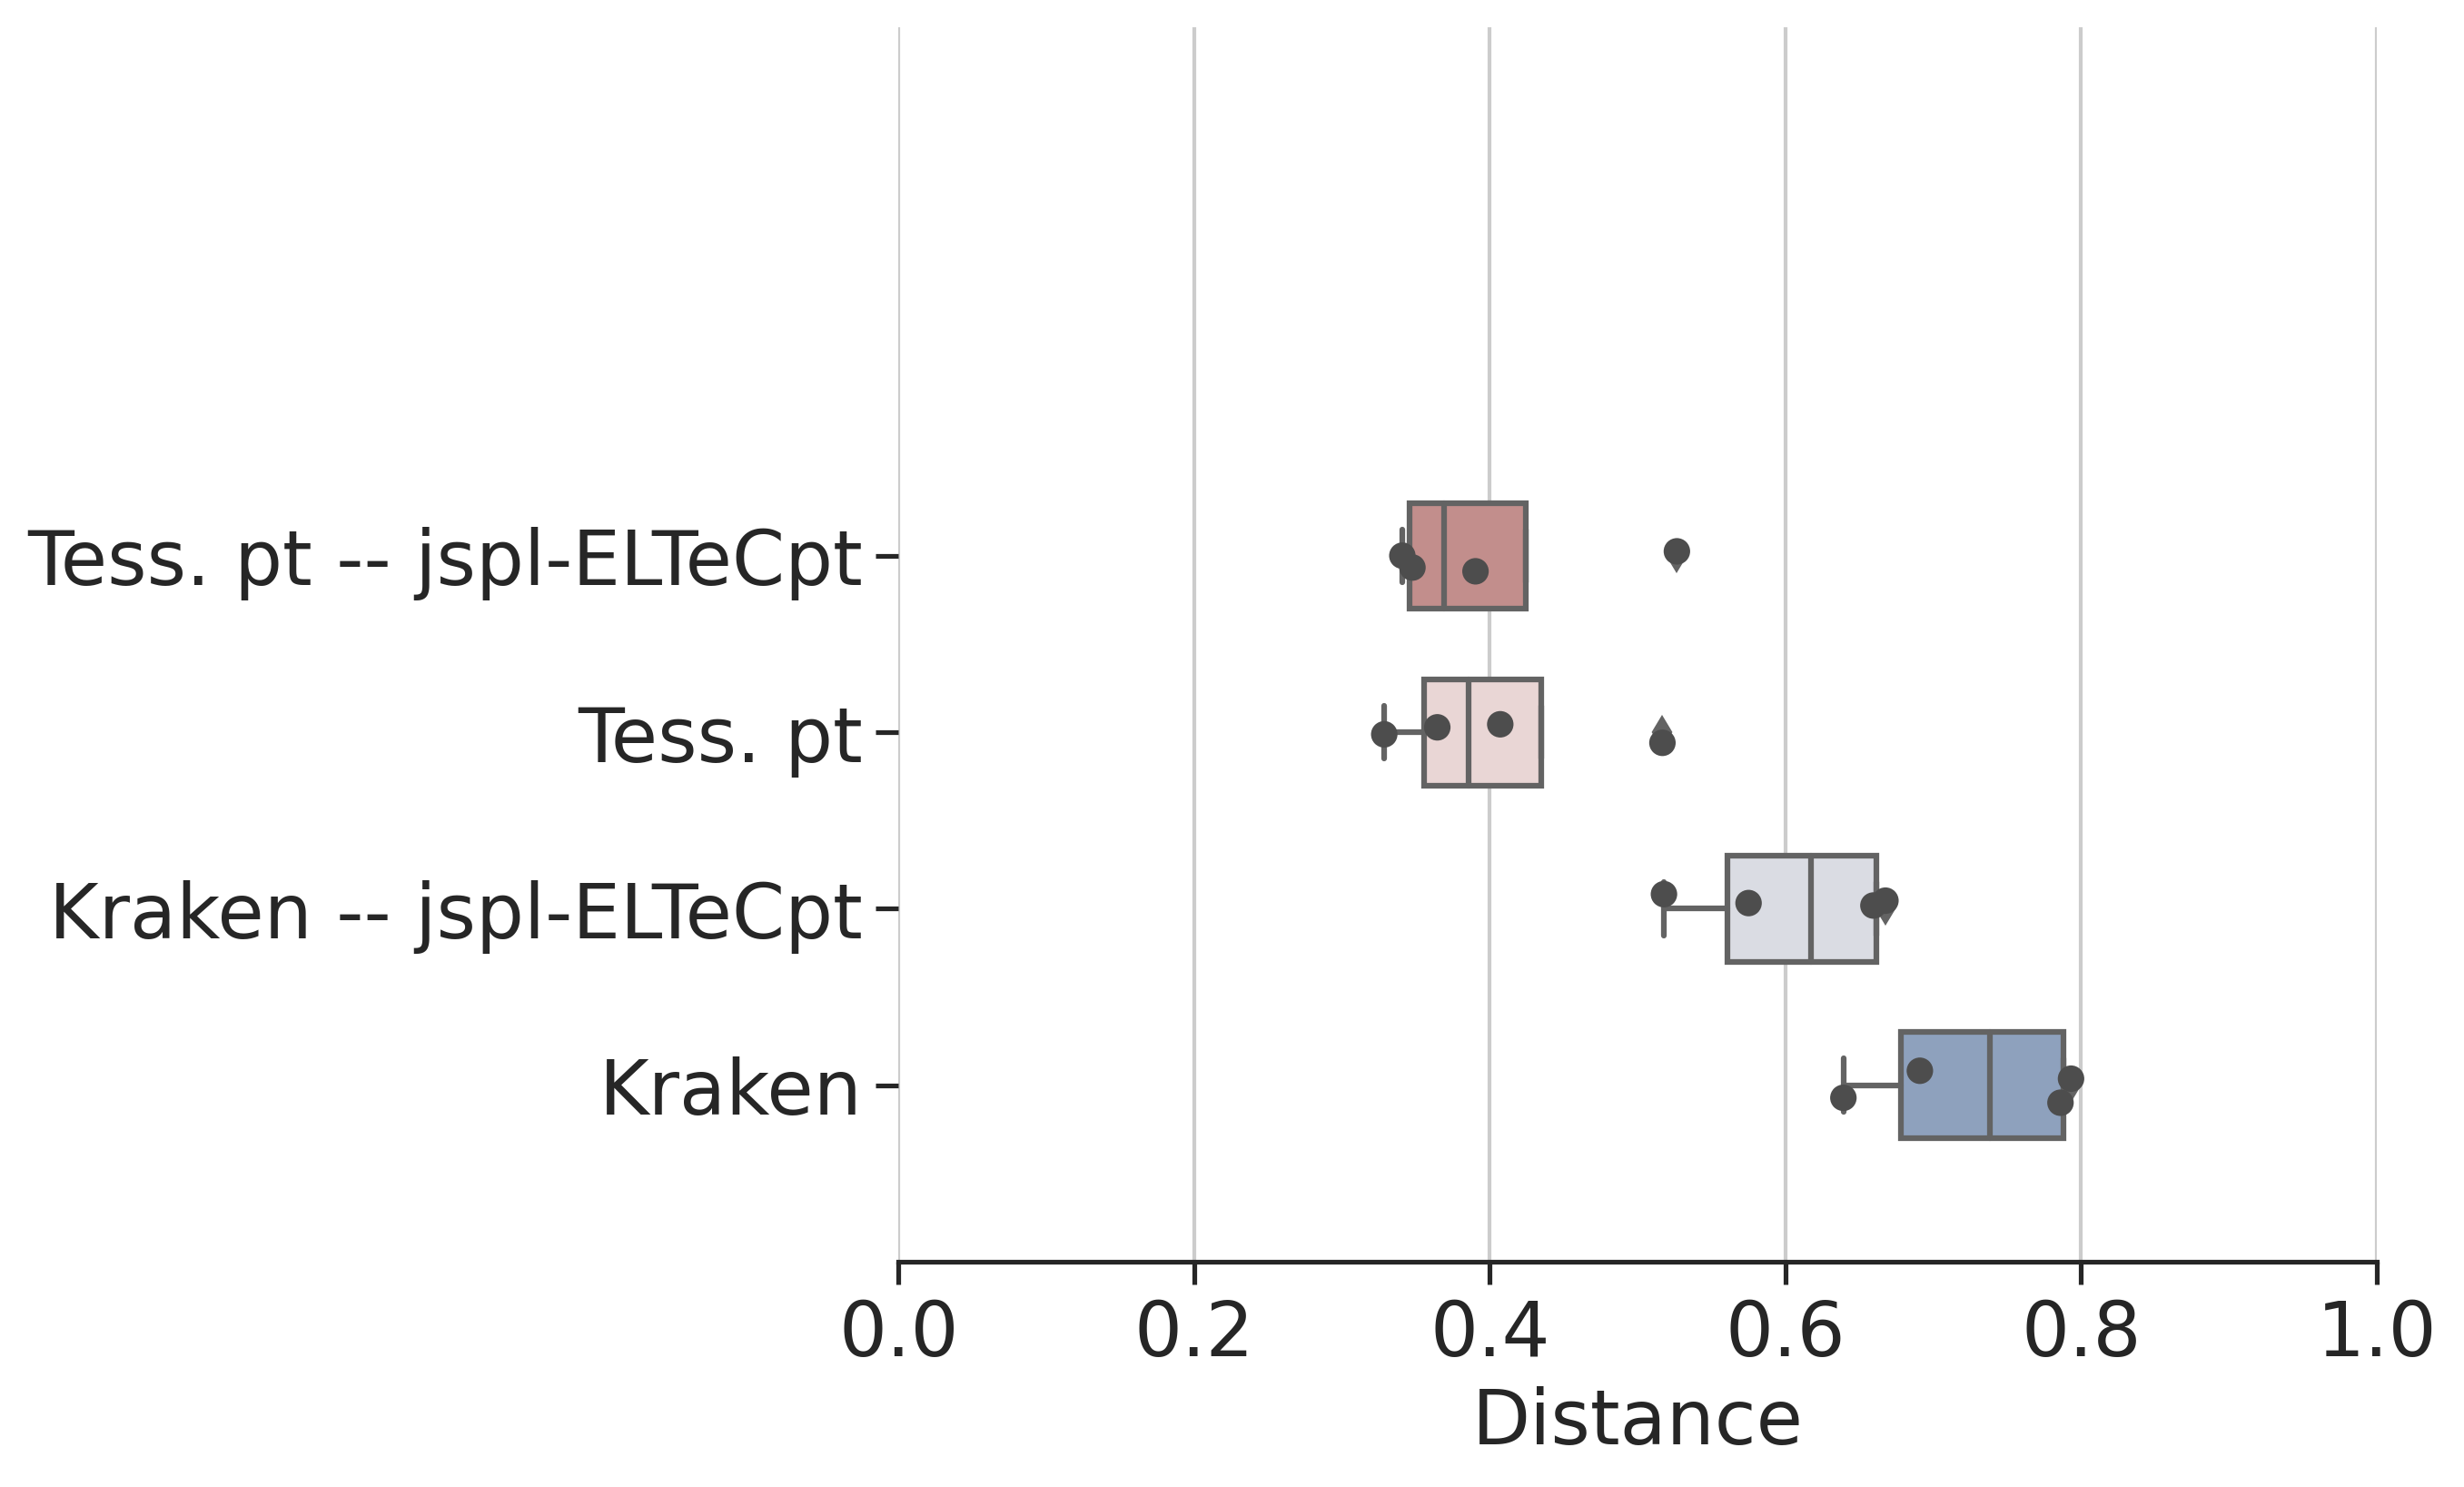
\includegraphics[height=.65\textwidth]{IMAGES/Boite-moustache/ELTeC-Por_REF_jaccard.png} 
        \caption{ELTeC-Por Jaccard}
        \label{fig:ELTeC-Por_REF_jaccard}
   \end{subfigure}
    \begin{subfigure}{0.5\textwidth}
  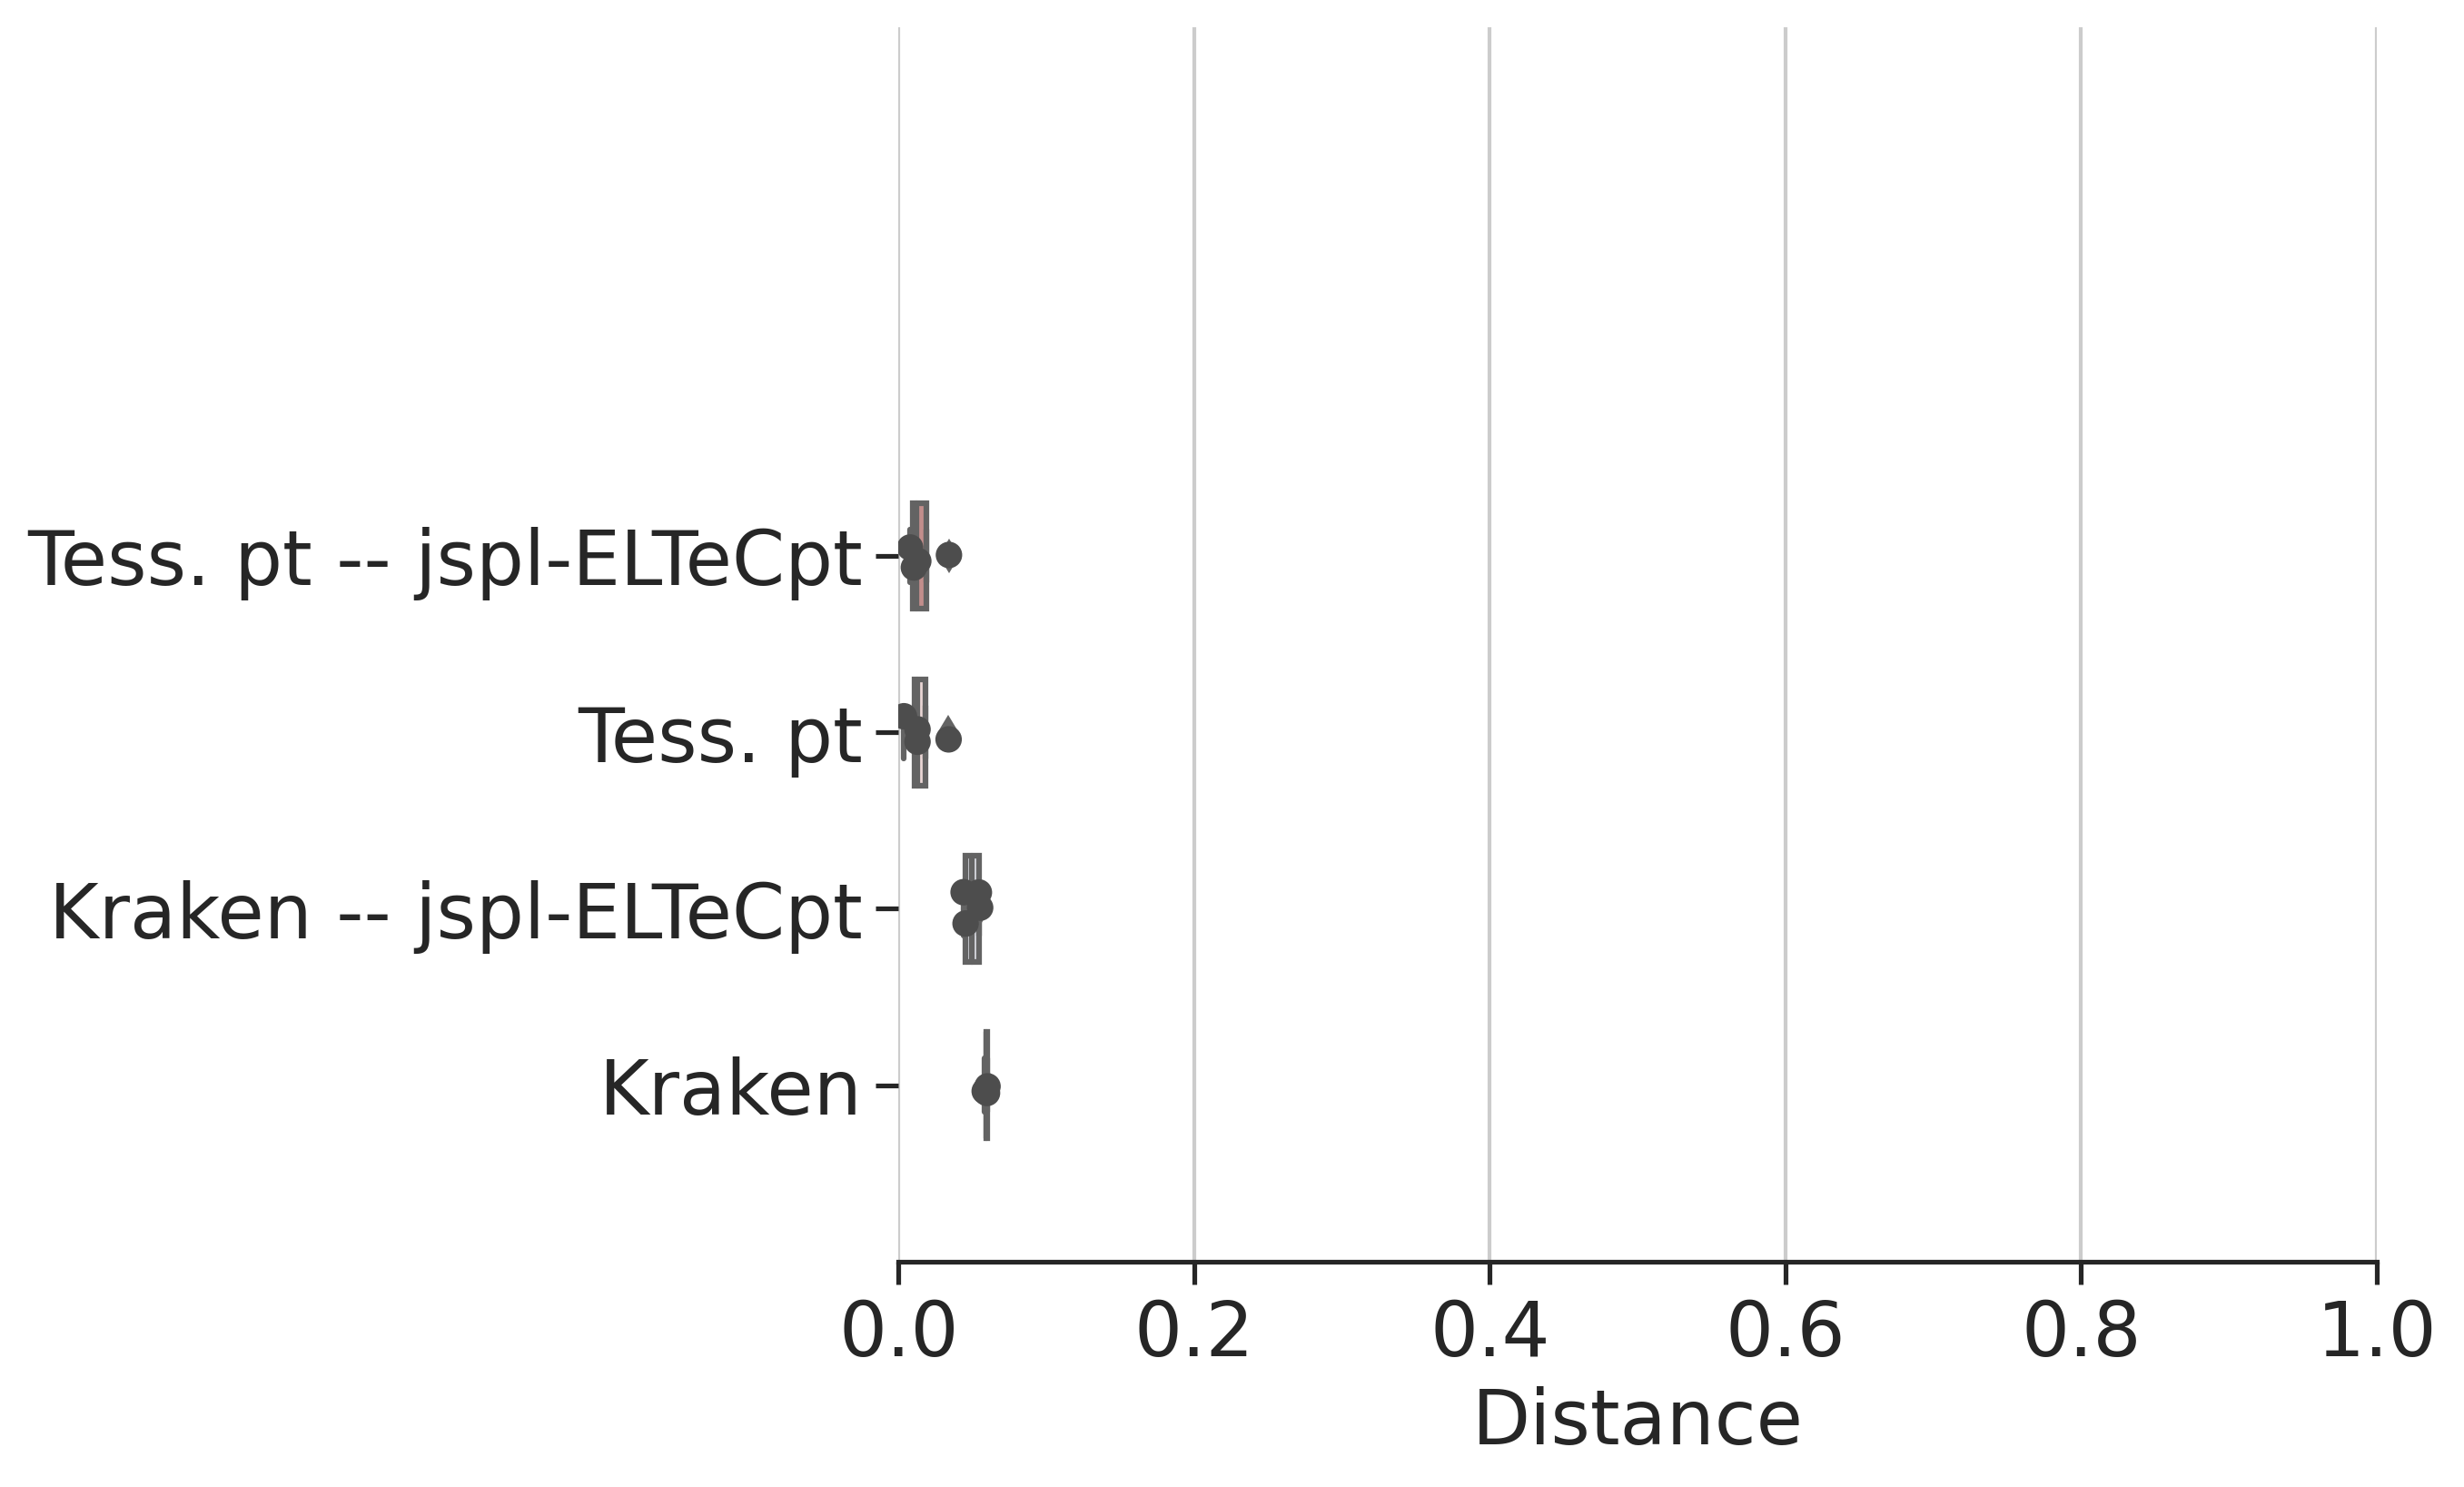
\includegraphics[height=.65\textwidth]{IMAGES/Boite-moustache/ELTeC-Por_REF_cosinus.png} 
        \caption{ELTeC-Por cosinus}
        \label{fig:ELTeC-Por_REF_cosinus}
   \end{subfigure}   
%    \caption{Distances calculées entre les textes de référence et les versions de ROC.}
\label{fig:distance_texte}
%\end{figure}

%%% TODO GL: Alignement des figures boites à moustache
%\begin{figure}
%   \centering
         \begin{subfigure}{0.45\textwidth}
  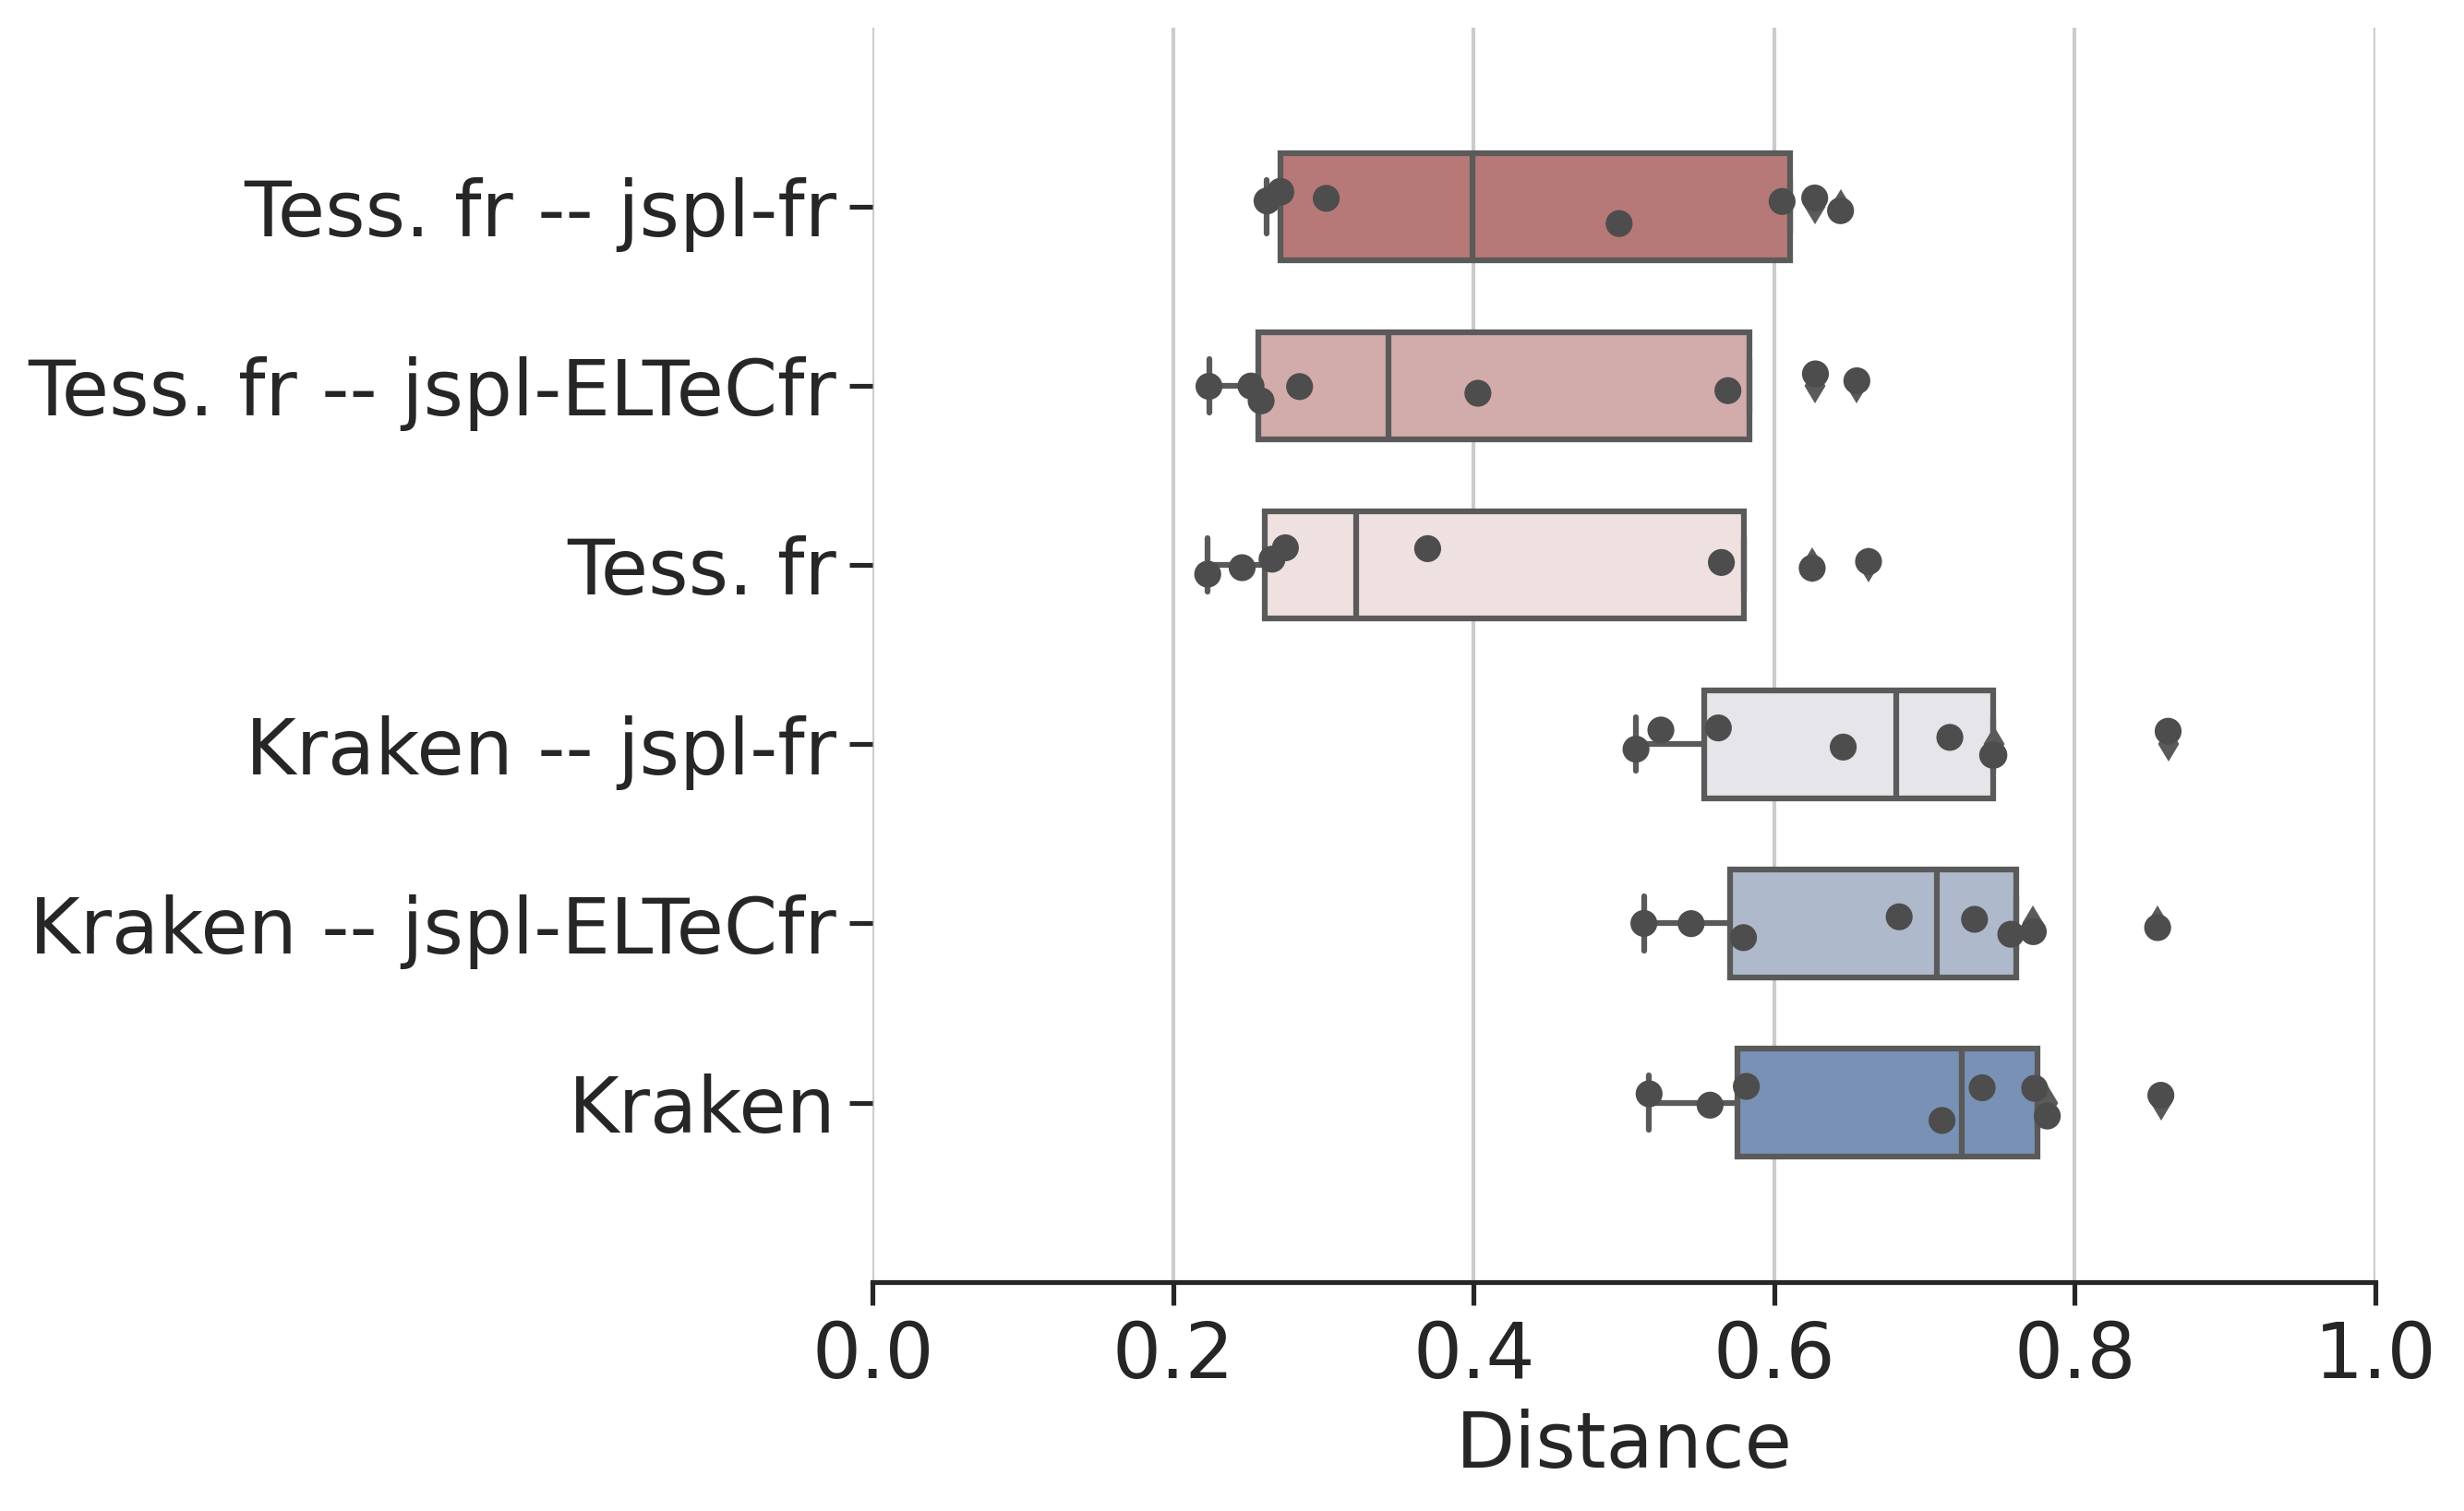
\includegraphics[height=.65\textwidth]{IMAGES/Boite-moustache/TGB_REF_jaccard.png} 
        \caption{TGB Jaccard}
   \end{subfigure}
    \begin{subfigure}{0.5\textwidth}
  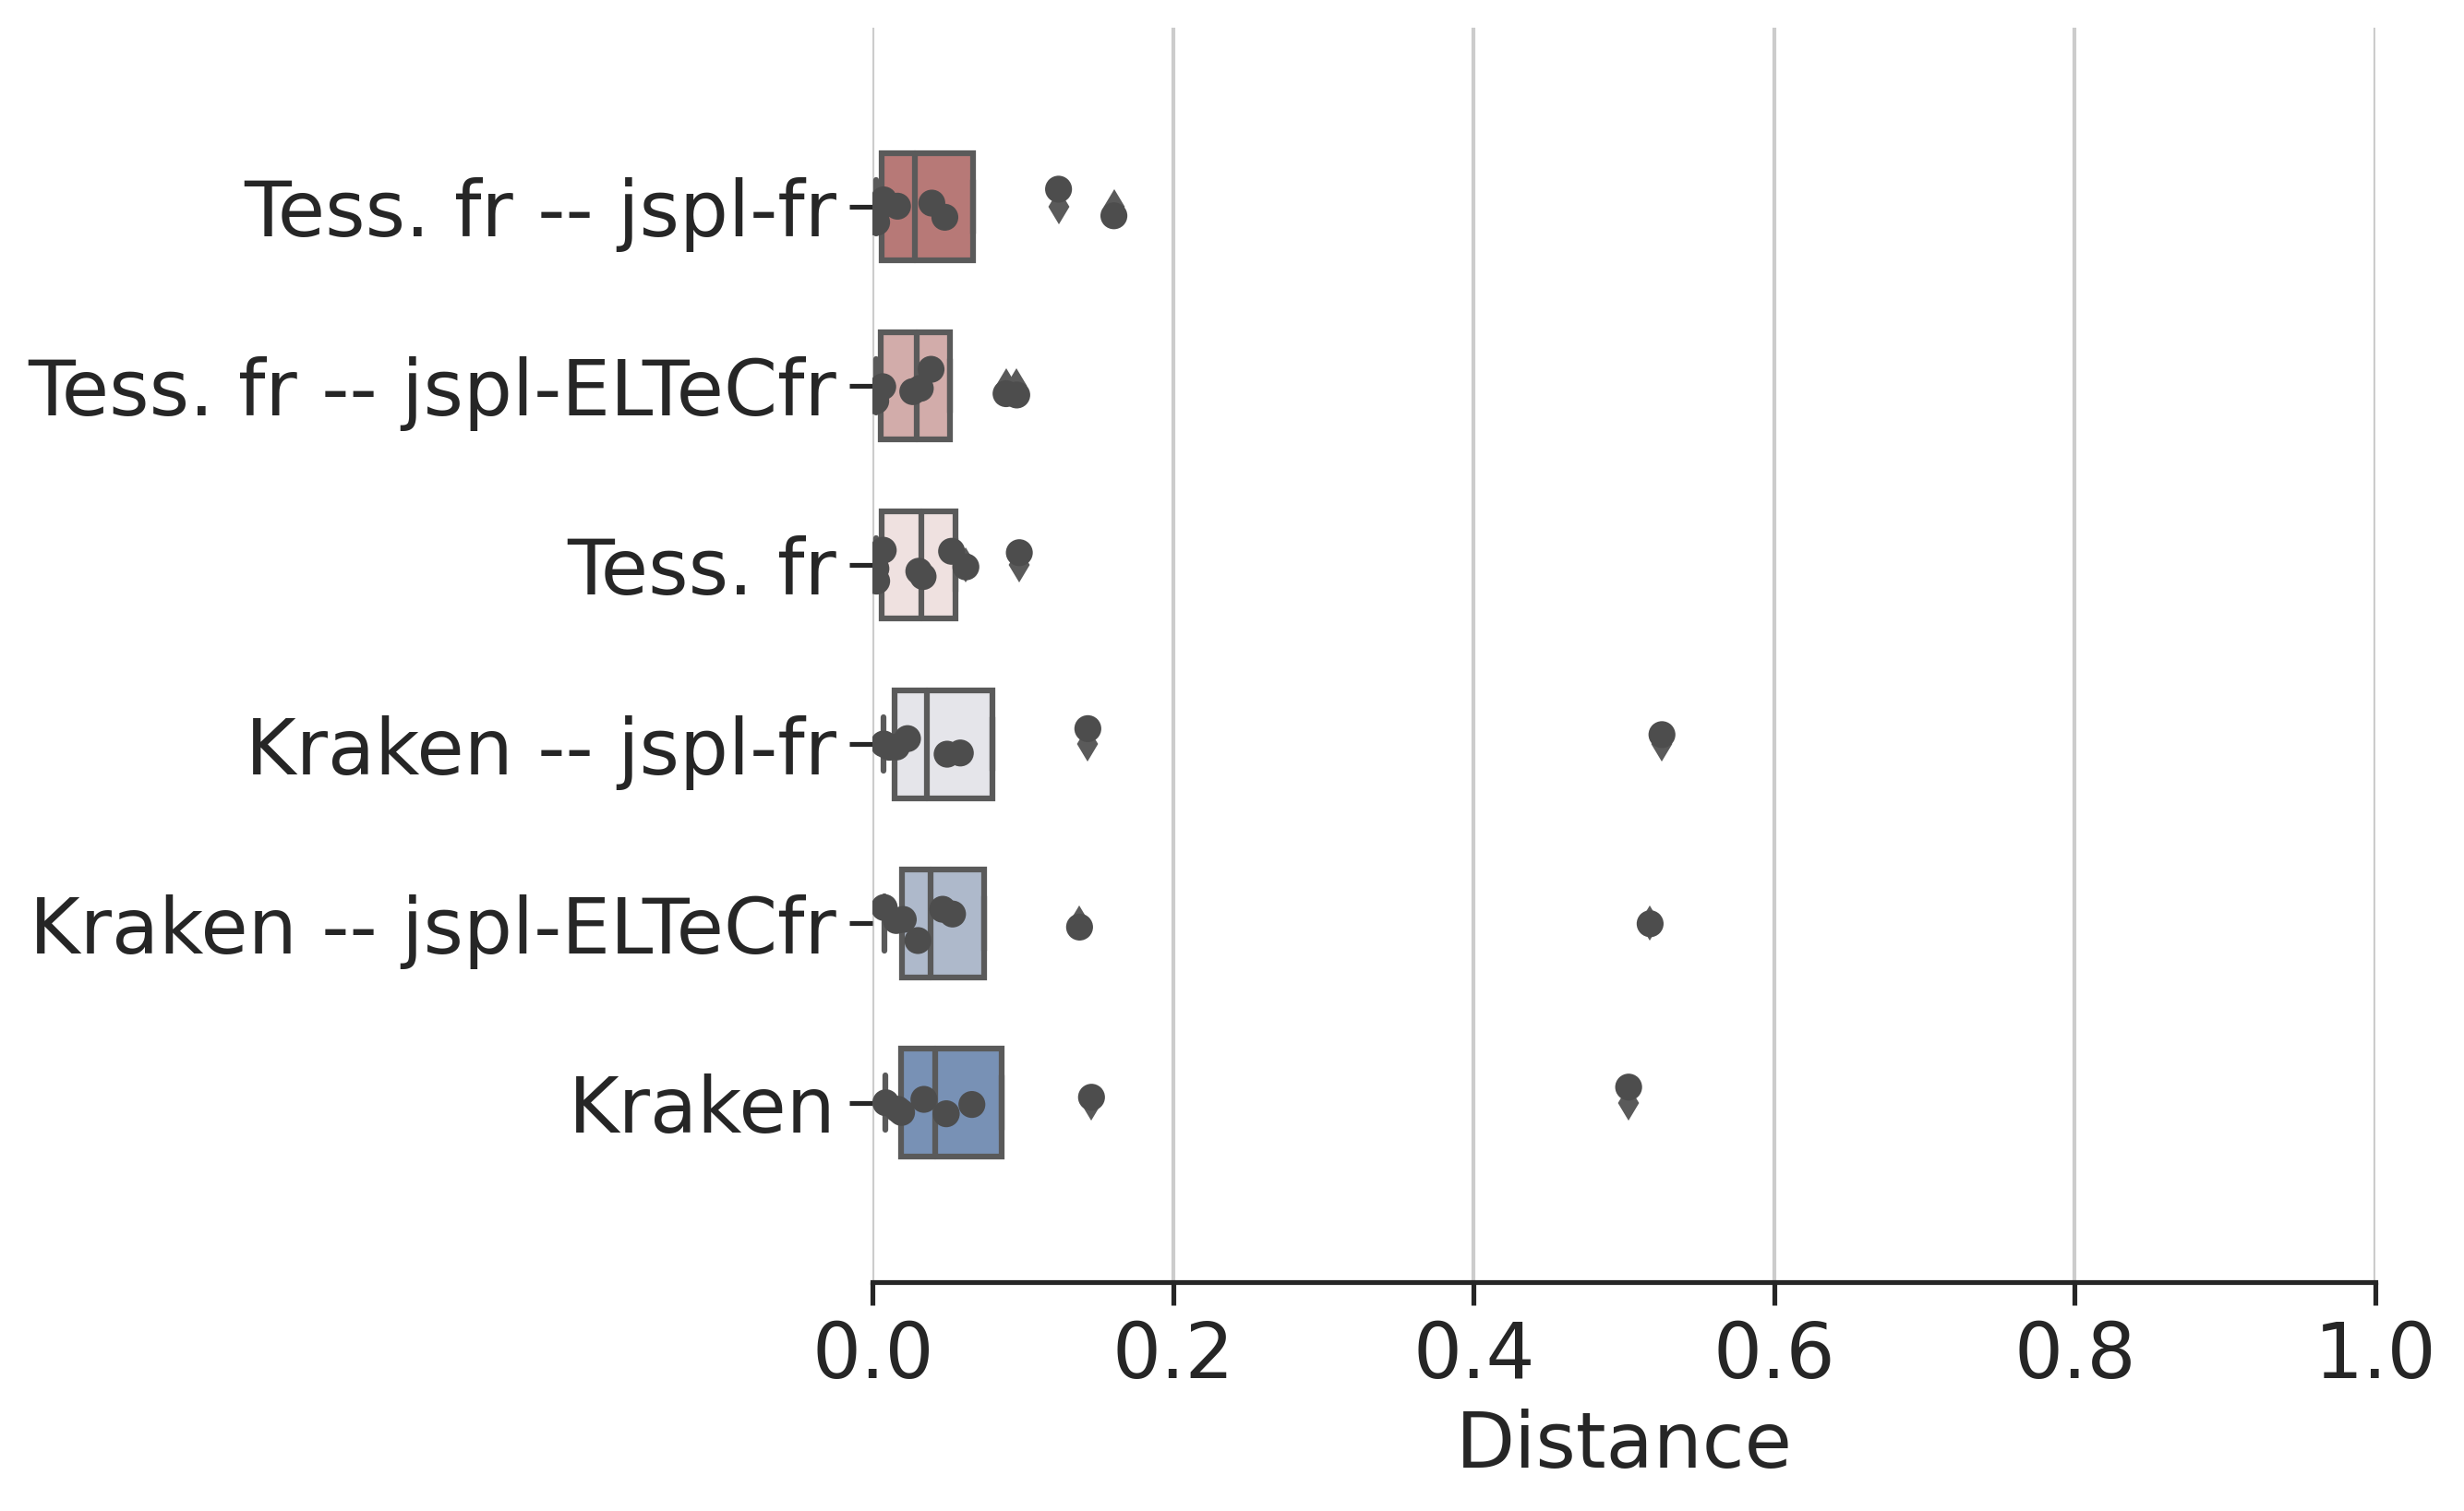
\includegraphics[height=.65\textwidth]{IMAGES/Boite-moustache/TGB_REF_cosinus.png} 
        \caption{TGB cosinus}
   \end{subfigure}
   
    \caption{Distances calculées entre les textes de référence et les versions de ROC.}
    \label{fig:distances_ref_roc}
\end{figure}

Les figures \ref{fig:distances_ref_roc} et \ref{fig:Cosinus-spacy-lg} montrent les résultats obtenus en comparant les sorties de REN obtenues sur les textes de référence et celles des différentes configurations évaluées (tableau \ref{tab:config}). Pour lire ces figures, il faut noter que plus la boîte est proche de zéro, plus les sorties comparées sont similaires.
Après une observation des différentes mesures de distance présentées pour chaque sous-corpus évalué, on note l'écart constant et considérable entre les résultats de Jaccard et cosinus. Les résutats pour Jaccard sont souvent proches de 1, tandis que ceux de cosinus sont proches de 0 pour les comparaisons des mêmes configurations. Il semble que la métrique cosinus sous-estime la distance entre les résultats pour les configurations de ROC et celles de référence. 

\begin{figure}[h!]

    \begin{subfigure}{0.45\textwidth}
  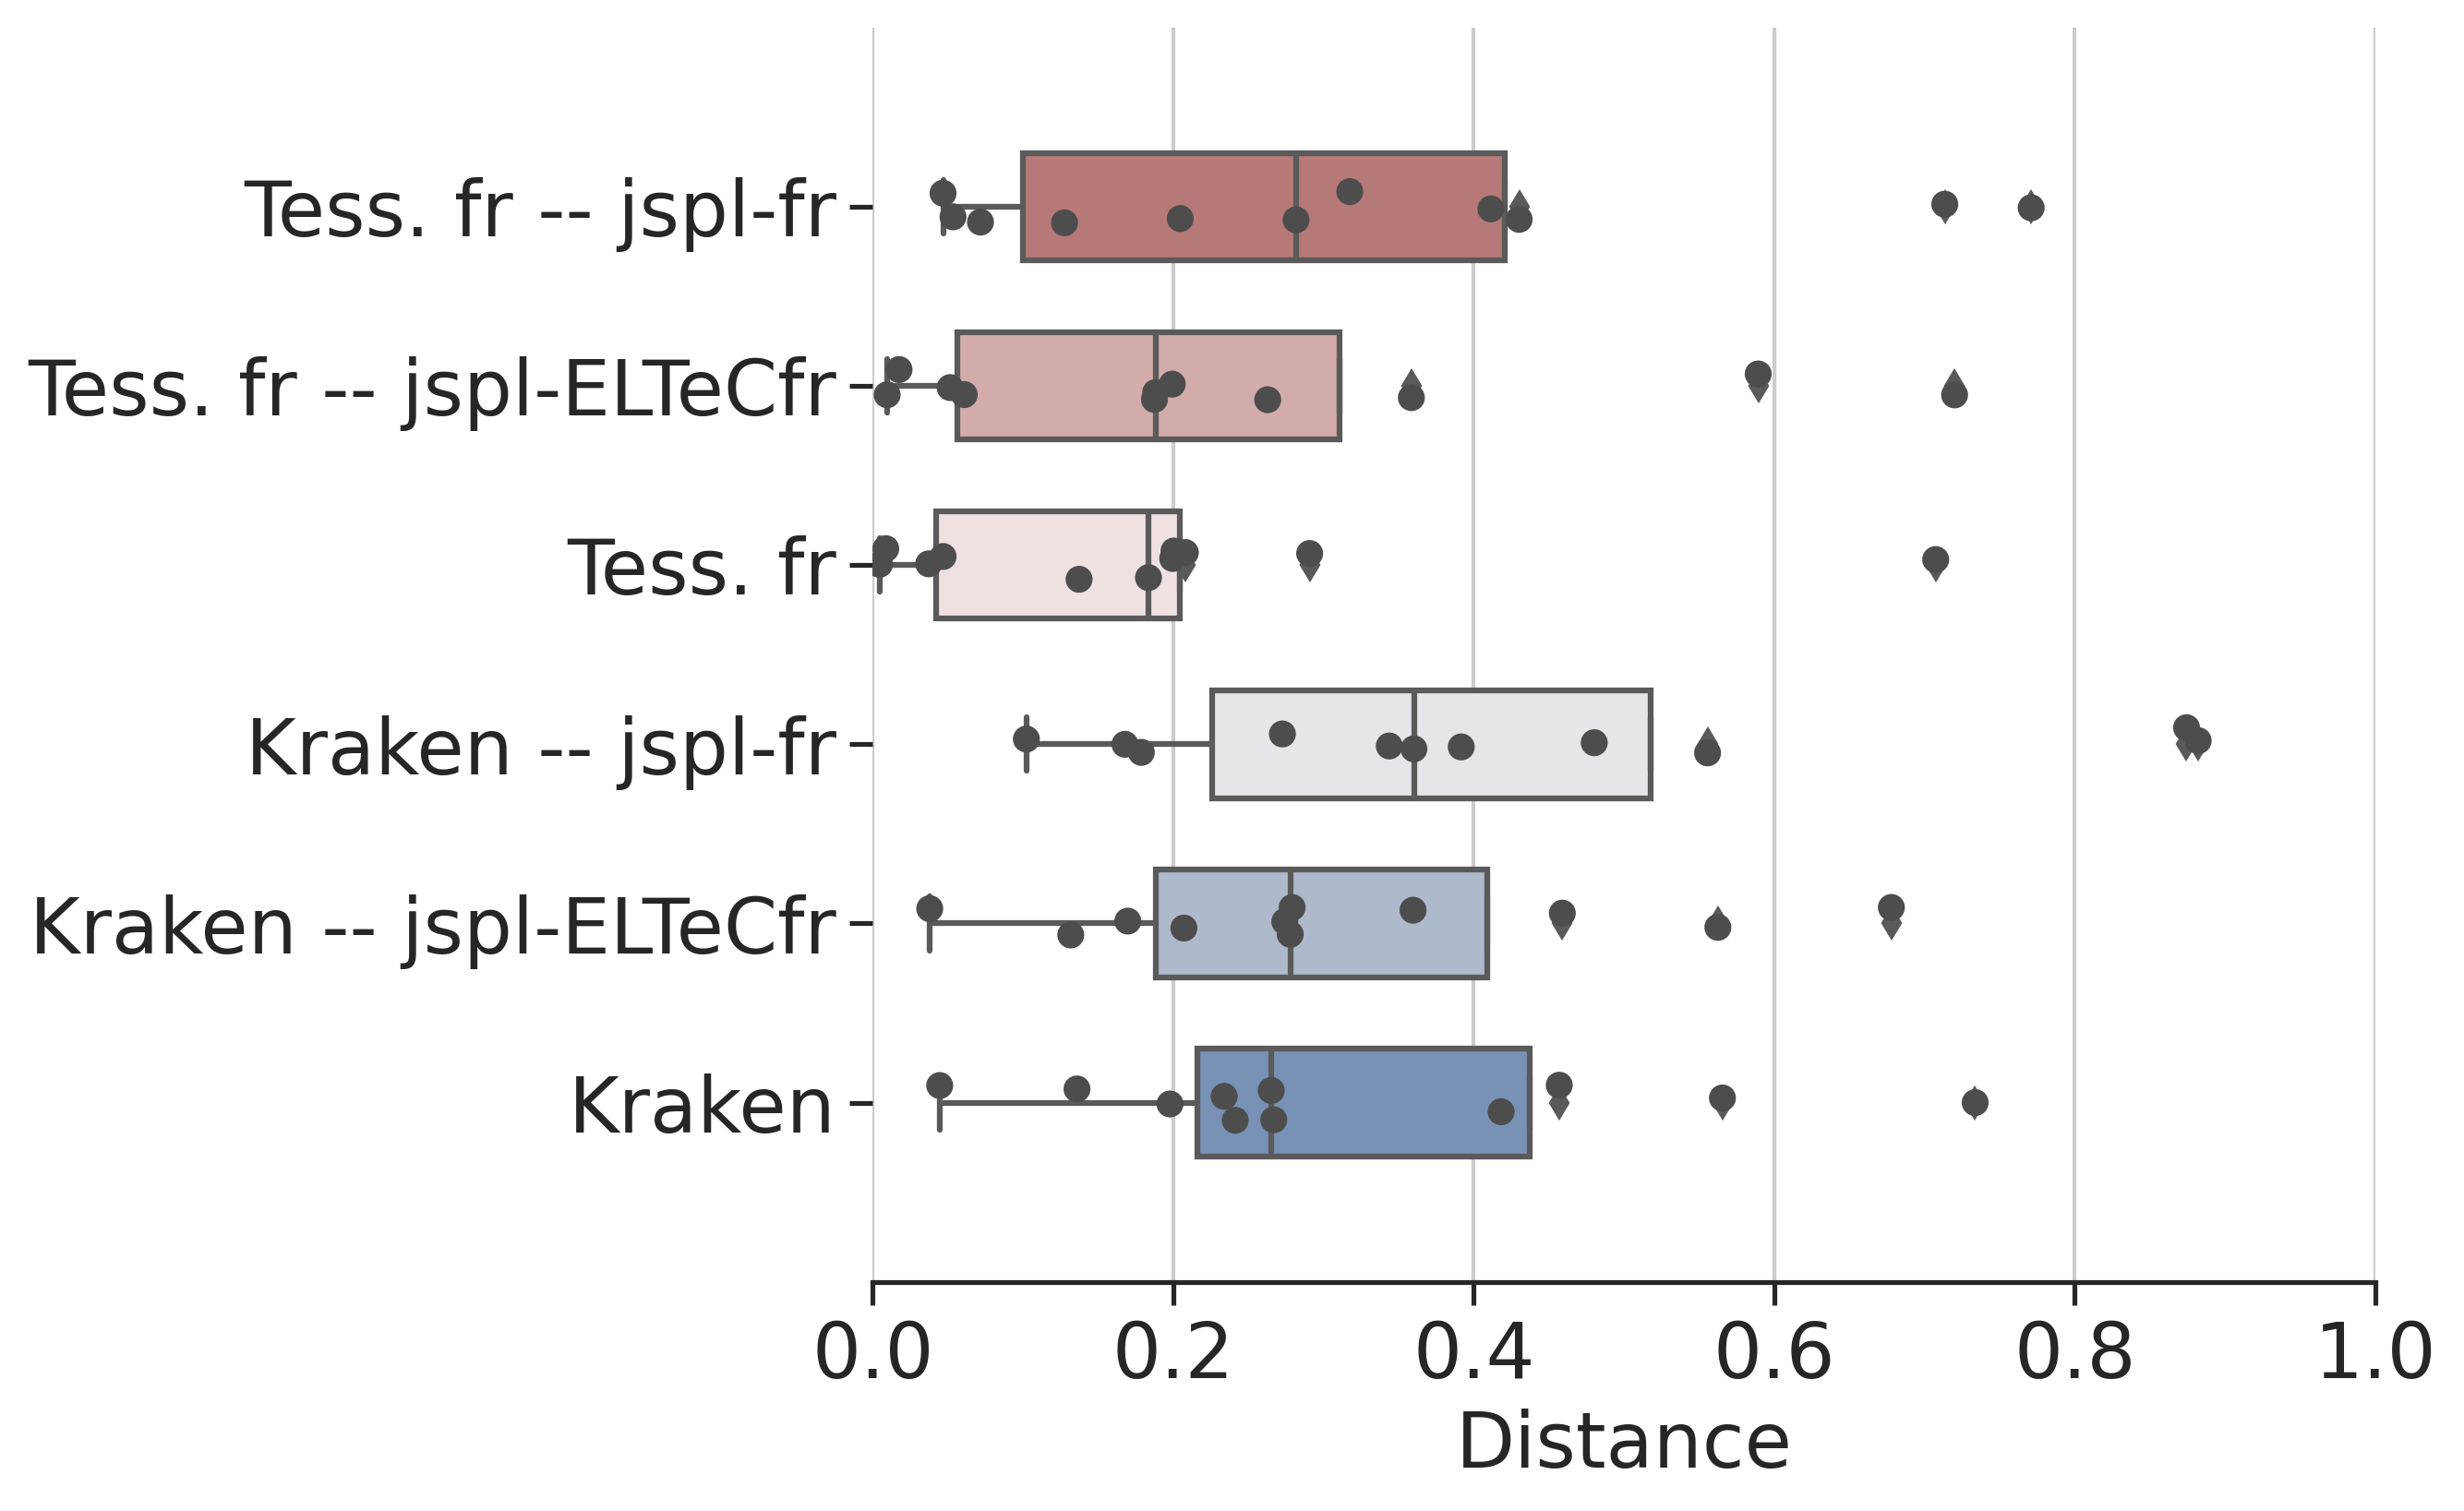
\includegraphics[height=.65\textwidth]{IMAGES/Boite-moustache/ELTeC-Fra_spacy3.5.1_cosinus.png} 
        \caption{ELTeC-Fra \texttt{spaCy} cosinus}
   \end{subfigure}
 \begin{subfigure}{0.45\textwidth}
  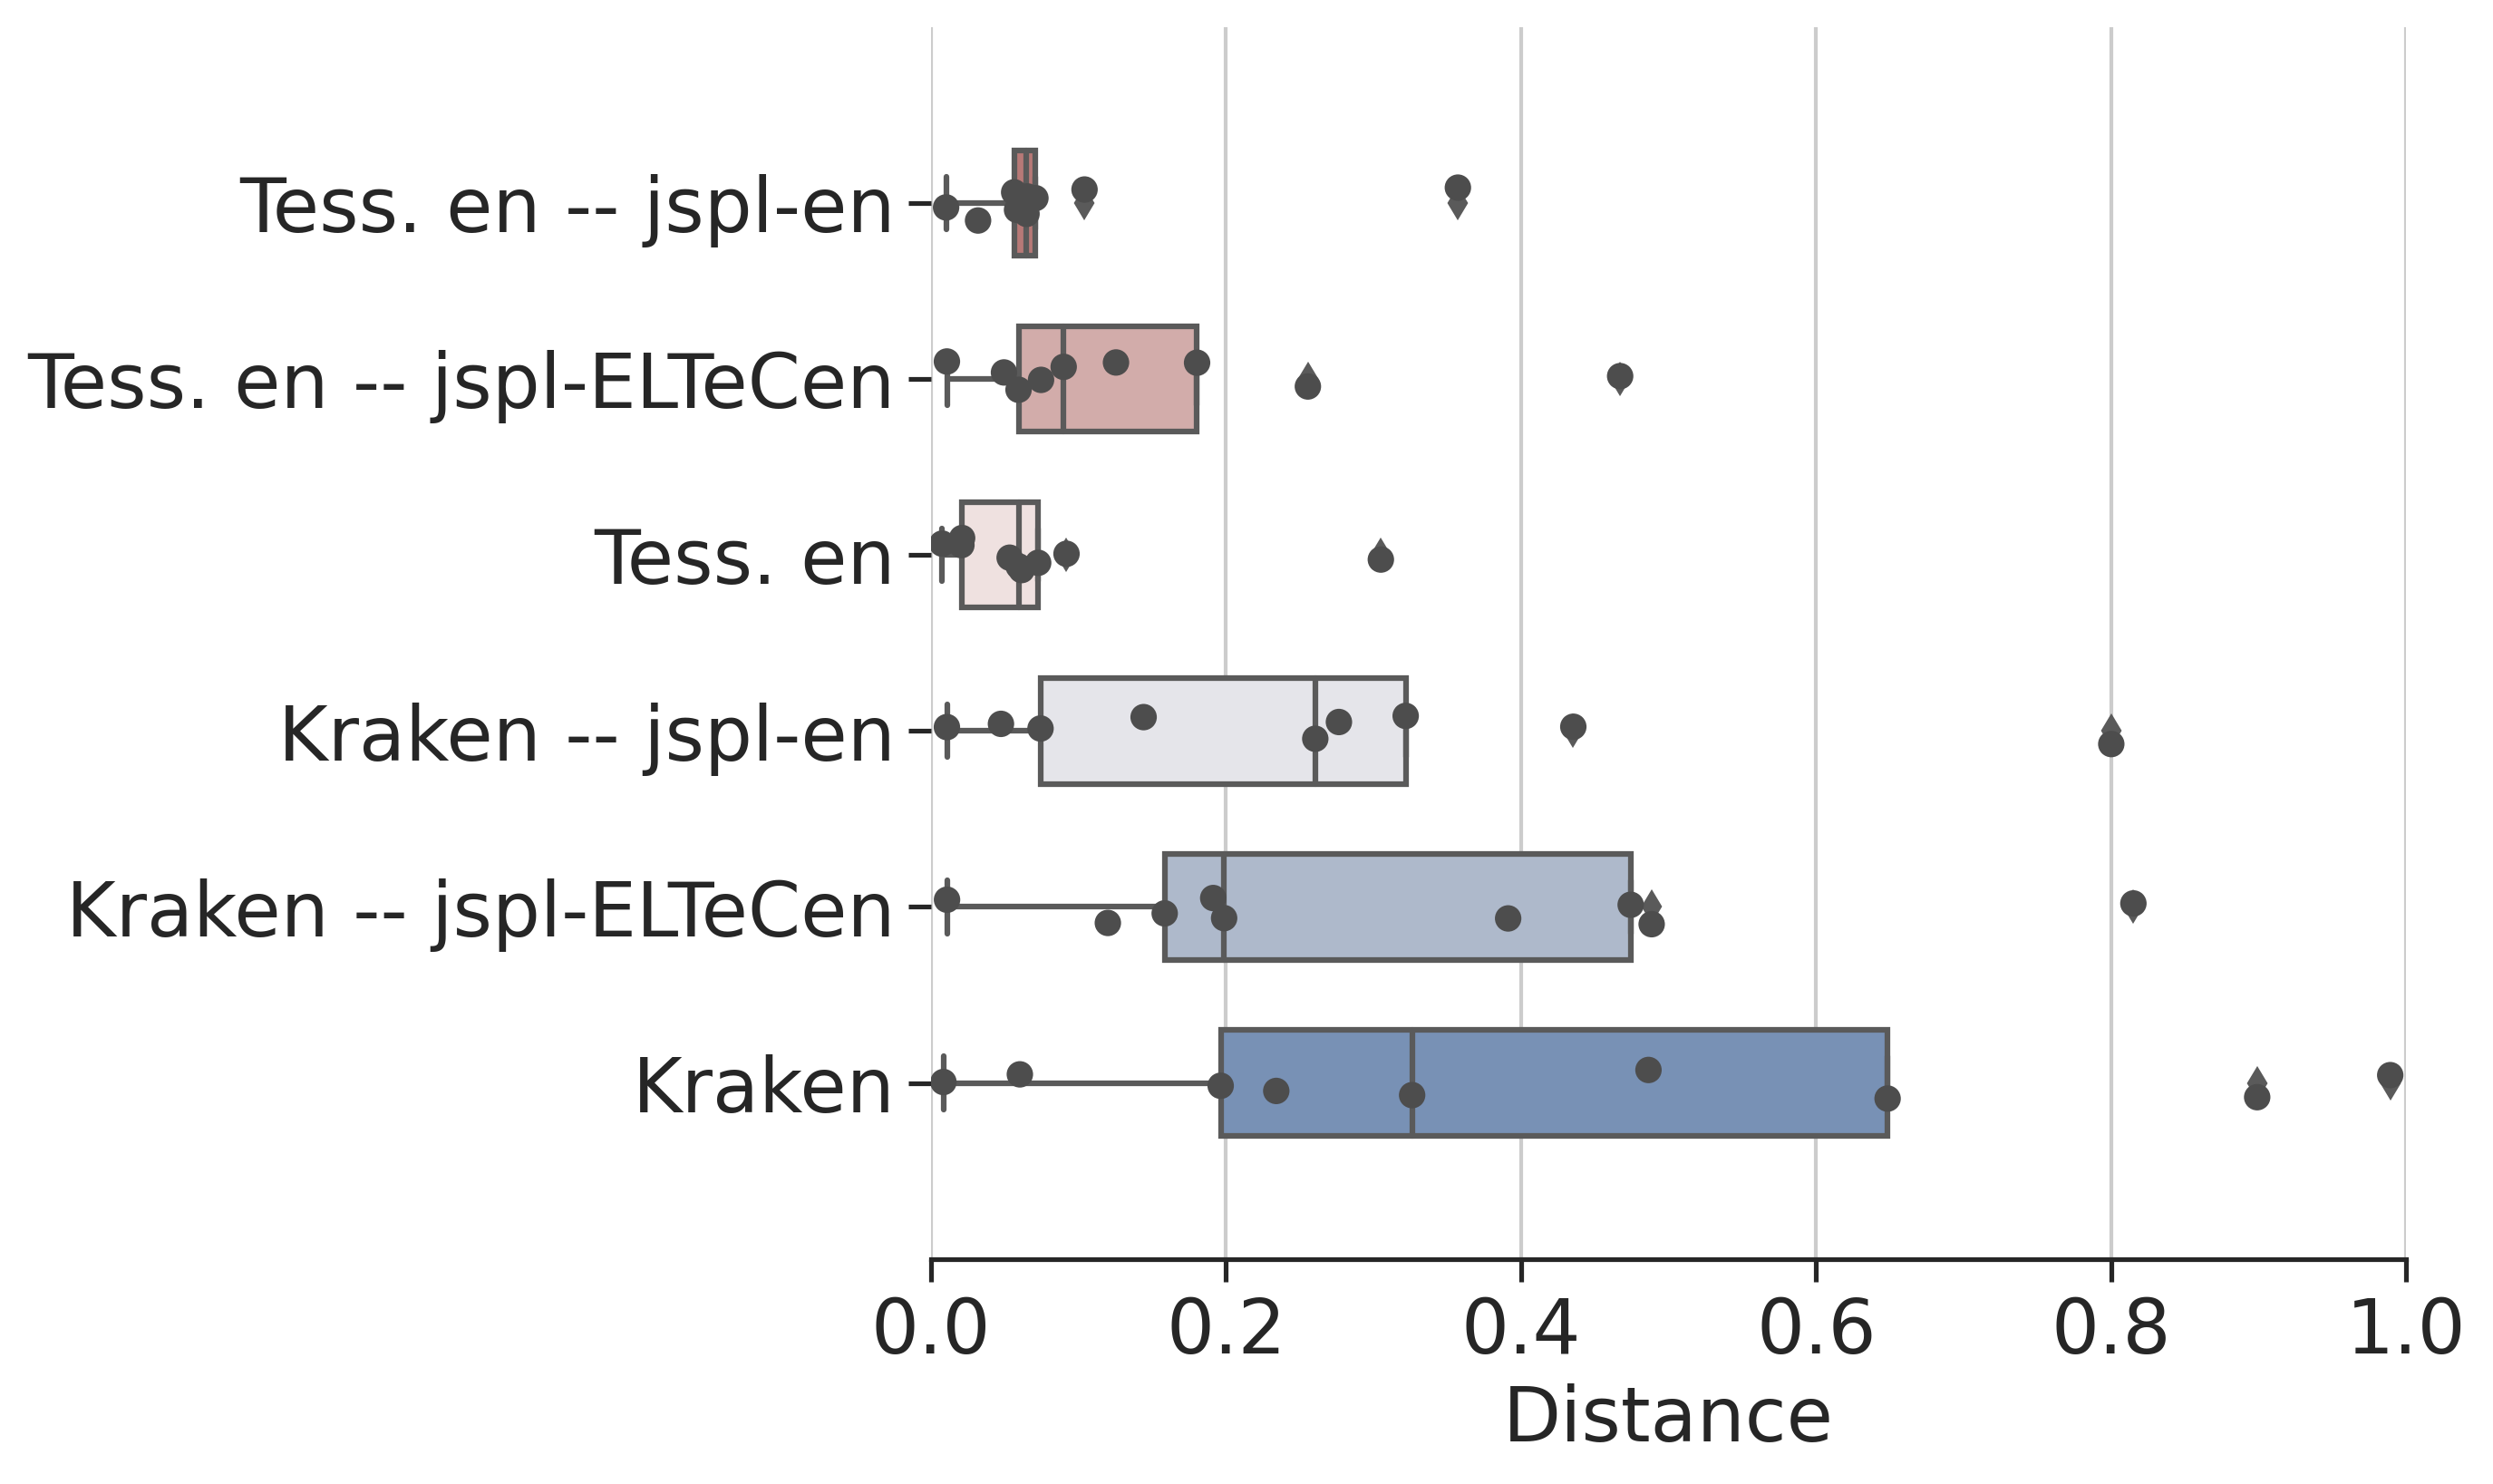
\includegraphics[height=.65\textwidth]{IMAGES/Boite-moustache/ELTeC-Eng_spacy3.5.1_cosinus.png}
        \caption{ELTeC-Eng \texttt{spaCy} cosinus}
   \end{subfigure}
    \begin{subfigure}{0.5\textwidth}
  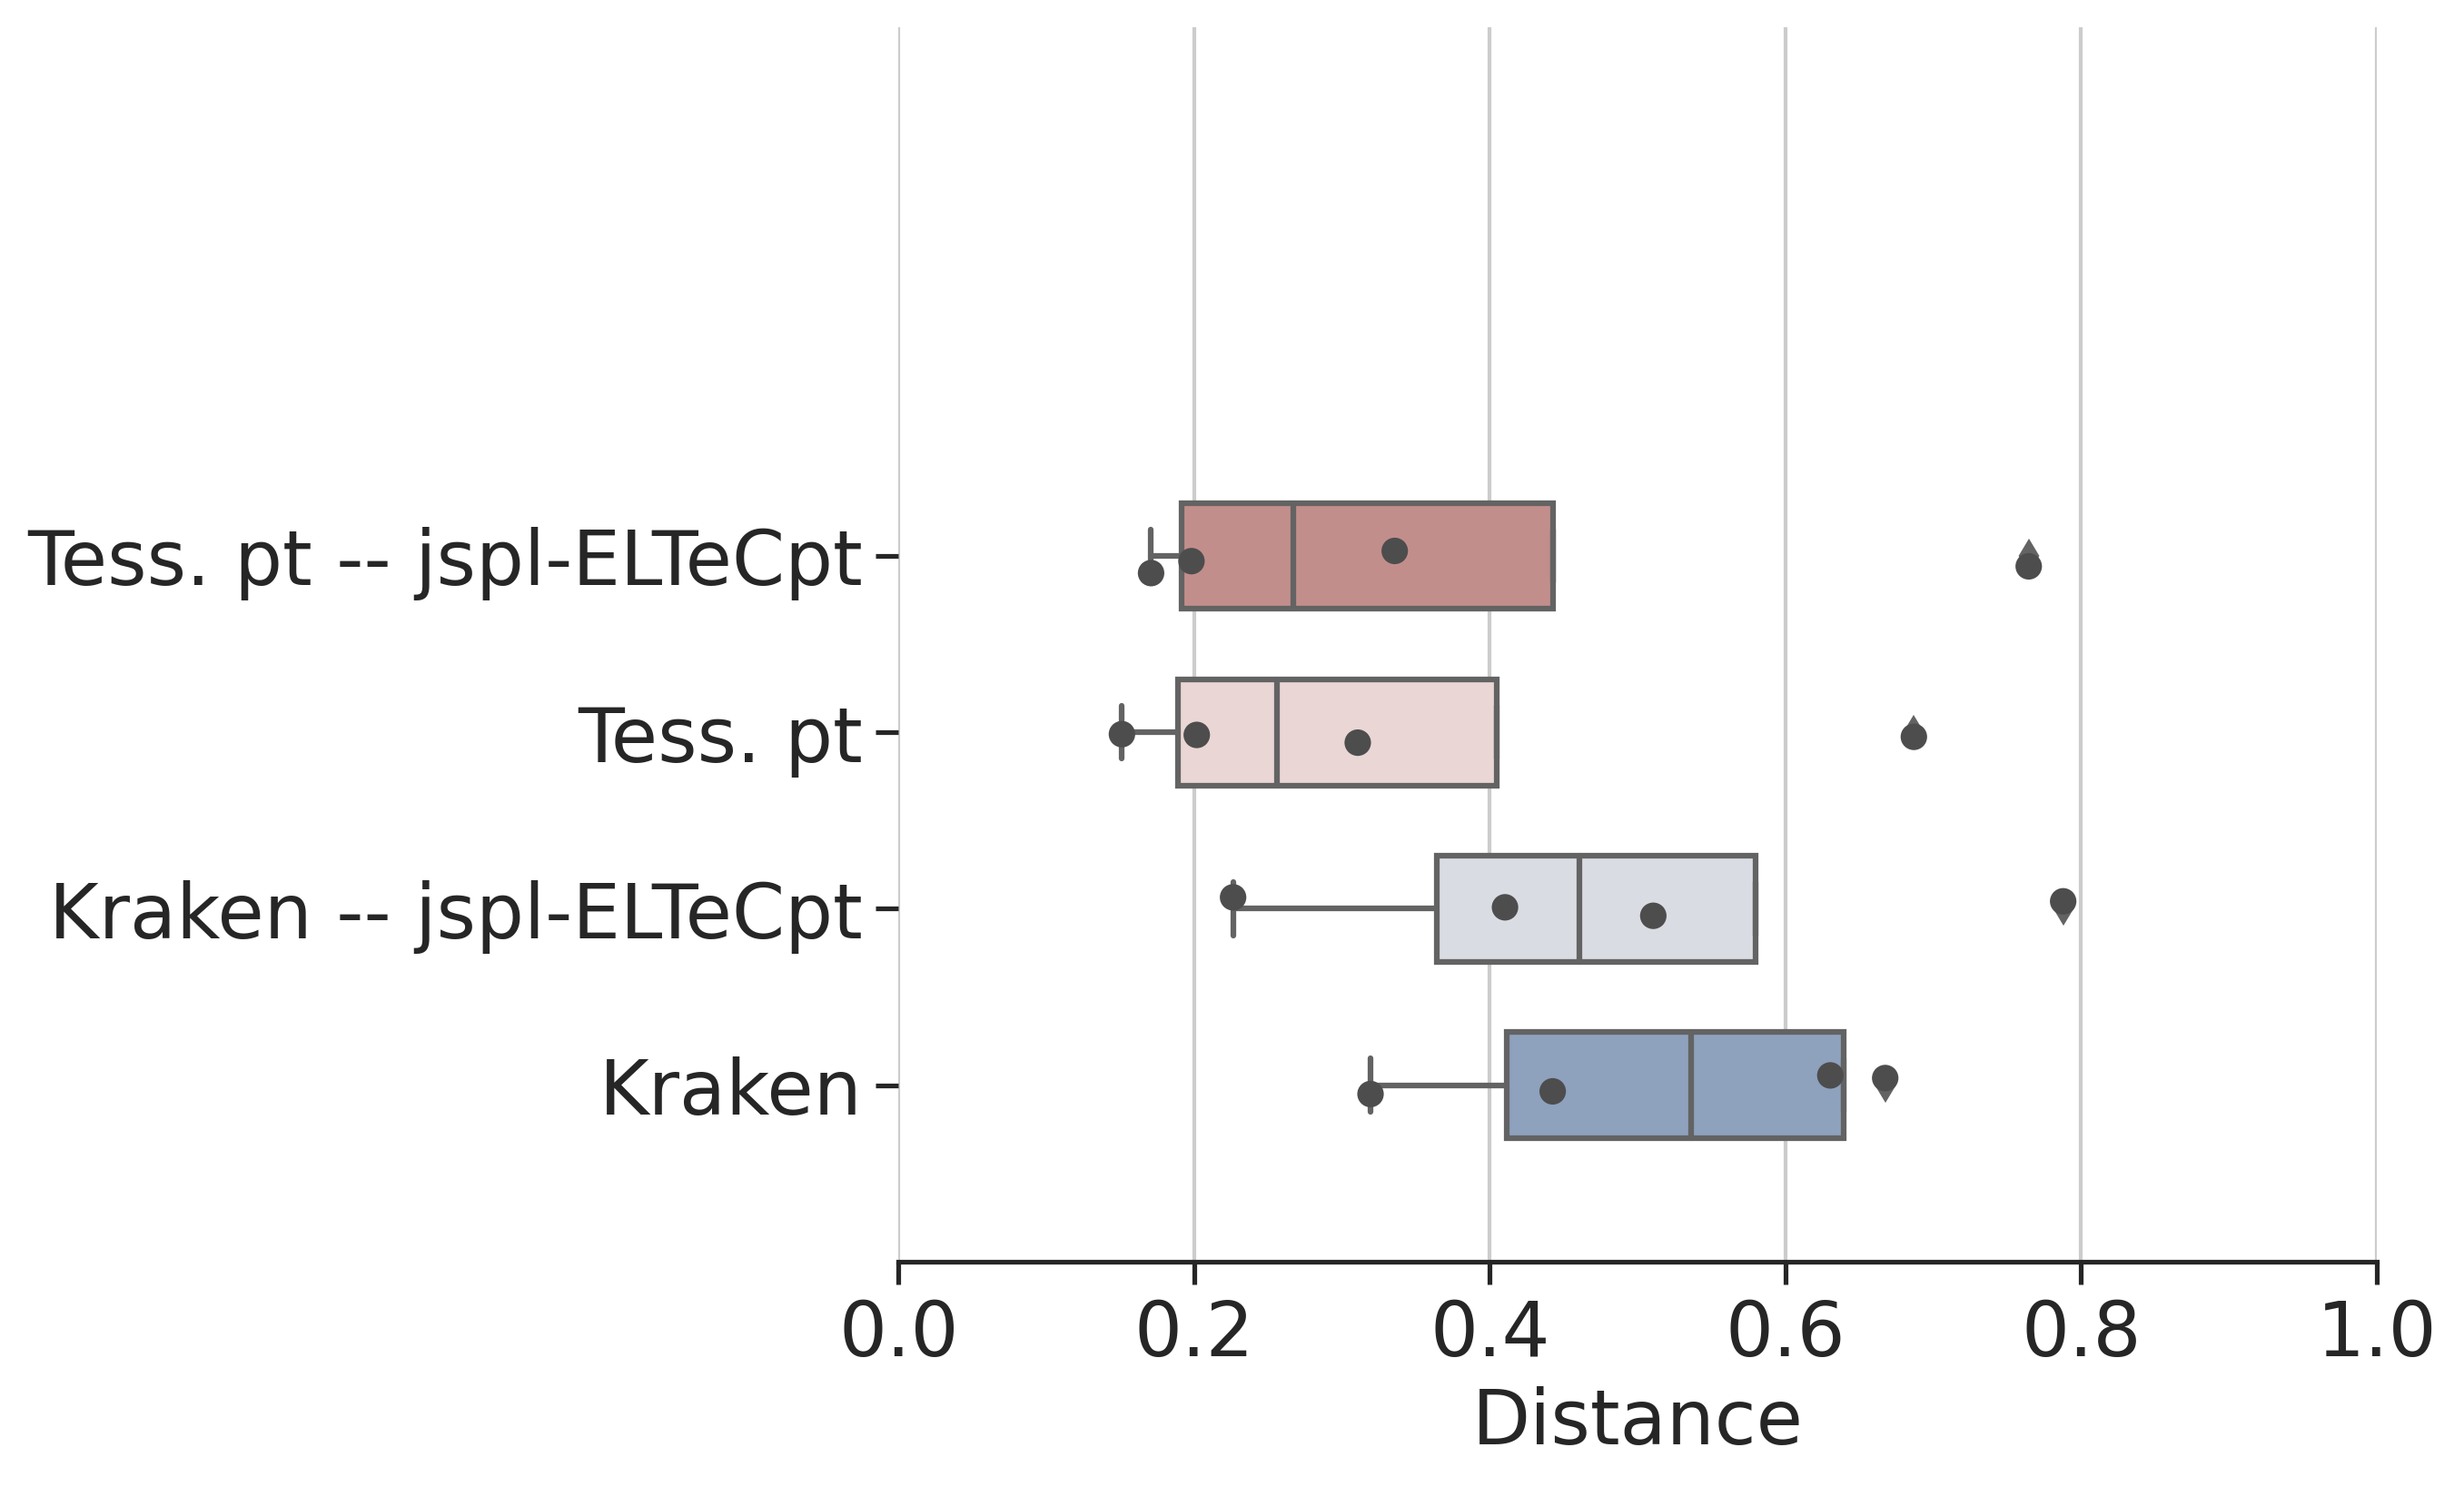
\includegraphics[height=.65\textwidth]{IMAGES/Boite-moustache/ELTeC-Por_spaCy3.5.1_cosinus.png} 
        \caption{ELTeC-Por \texttt{spaCy} cosinus} 
         \label{fig:ELTeC-Por-spaCy-cosinus}
   \end{subfigure}
     \begin{subfigure}{0.5\textwidth}
  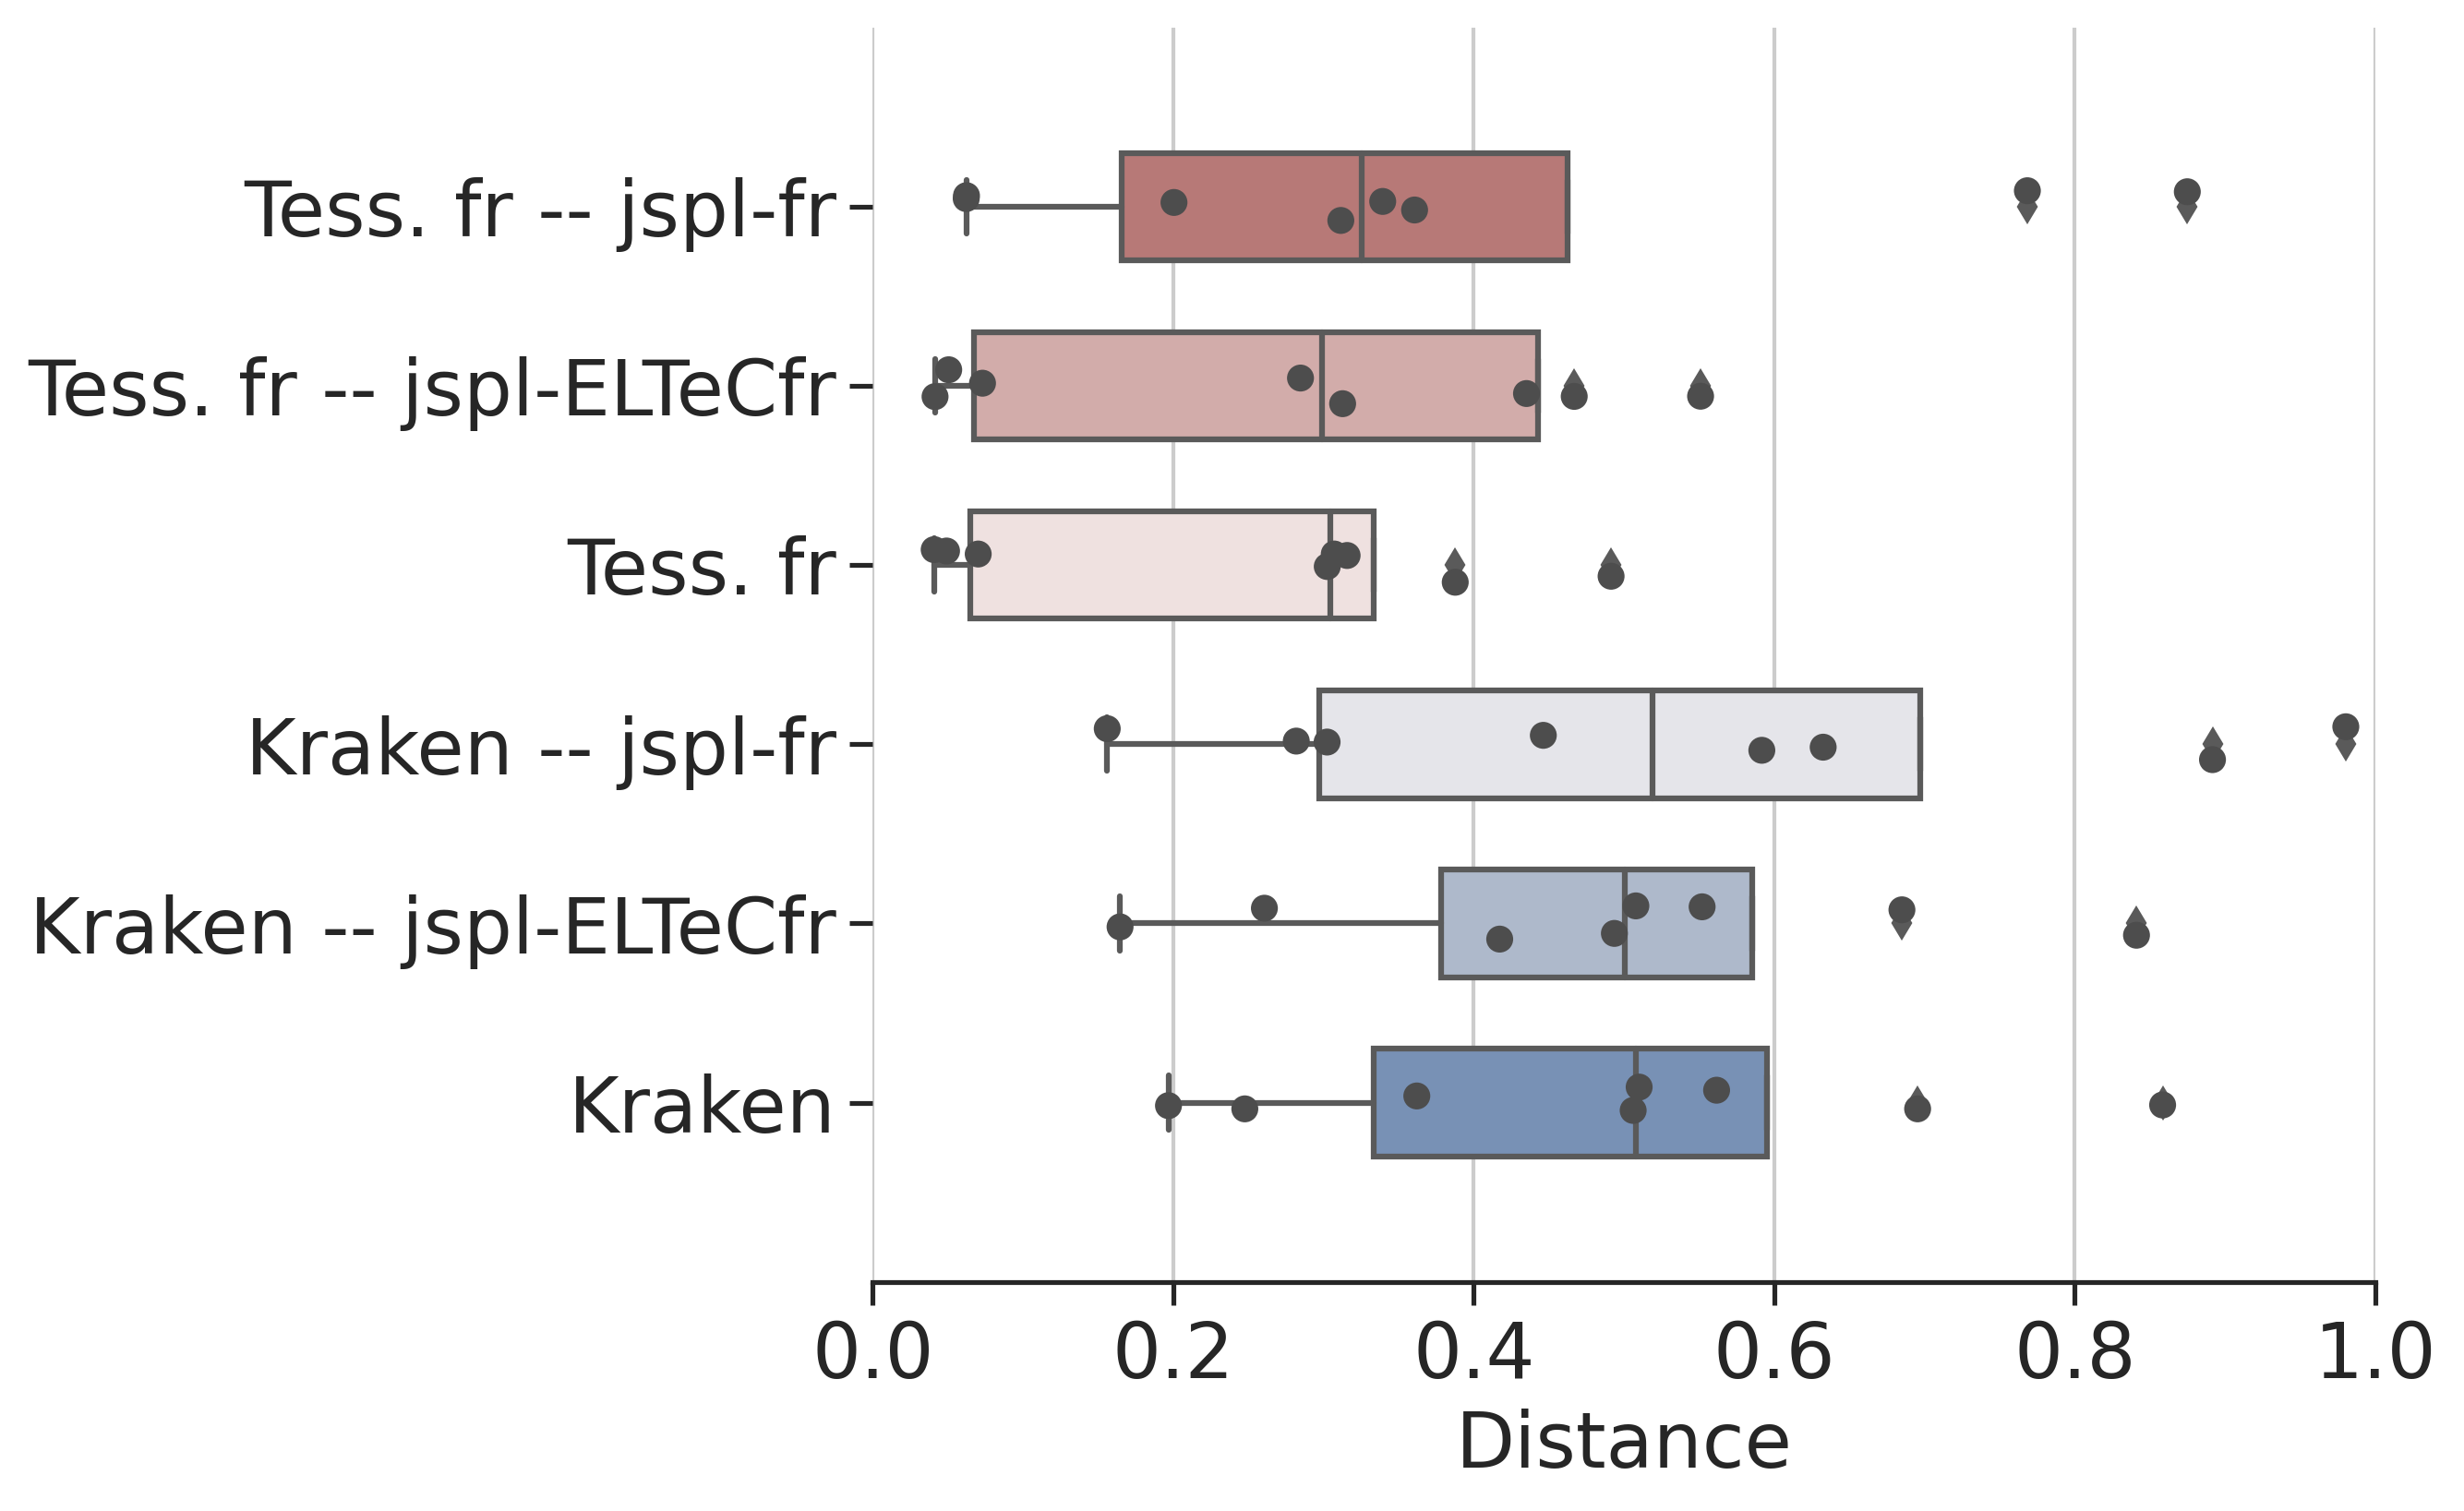
\includegraphics[height=.65\textwidth]{IMAGES/Boite-moustache/TGB_spaCy3.5.1_cosinus.png} 
        \caption{TGB \texttt{spaCy} cosinus}
   \end{subfigure}
    \caption{Distance Cosinus pour \texttt{spaCy\_lg} sur chaque sous-corpus globalement.}
%    \label{fig:Cosinus-spacy-lg-stanza}
\label{fig:Cosinus-spacy-lg}
\end{figure}


Pour préciser notre réflexion s'appuyant sur la lecture des figures \ref{fig:distances_ref_roc} et \ref{fig:Cosinus-spacy-lg},
% et \ref{fig:Cosinus-spacy-lg-stanza} 
nous avons procédé à la lecture des figures obtenues pour chacun des autres corpus et consulté manuellement les résultats effectifs de REN. Finalement, cette différence entre les résultats de Jaccard et cosinus pourrait s'expliquer par le fait que la première mesure prend en compte le vocabulaire, alors que la seconde s'intéresse au nombre d'occurrences d'une EN. Concrètement, cela signifie pour la distance de Jaccard que si le vocabulaire entre les sorties de deux ensemble pour les configurations comparées est très différent, le résultat est proche de 1. 
En revanche, les résultats pour la mesure cosinus dépendraient du nombre d'occurences de chaque EN dans les groupes comparés. Autrement dit, s'il y a beaucoup d'occurrences d'une EN dans une des configurations comparée mais qu'elle n'apparaît pas en même quantité dans les résultats de la seconde configuration, les résultats pour cosinus grimpent en flèche. L'observation des résultats roman par roman pour la mesure cosinus nous permet d'étayer cette hypothèse, en effet on dénombre, p.\ ex.\, 290 occurrences du terme ``INGLEZA'' pour la configuration Tesseract-pt--\texttt{spaCy\_lg}, alors qu'il apparaît 3 fois seulement dans les résultats de la configuration de référence\footnote{\textit{Uma familia ingleza}, Diniz.} -- dans ce dernier cas la valeur de cosinus est très élevée et dépasse celle de Jaccard (cos. : 0.69, Jaccard : 0.67). Il s'agit d'un comportement que nous avons pu observer régulièrement dans les résultats pour chacun des sous-corpus analysés.

La figure \ref{fig:distances_ref_roc} laisse apercevoir que les résultats pour la REN sur les versions Kraken des textes sont moins bons de manière générale que pour les versions produites avec Tesseract. Toutefois, il semblerait que la correction automatique soit un peu plus efficace sur les versions de Kraken avec le modèle JamSpell-ELTeC que sur les versions Tesseract, car l'écart entre les boîtes est plus grand. Cependant, les résultats des distances obtenus pour ces versions corrigées de Kraken restent inférieurs à ceux observés pour les versions Tesseract avec et sans corrections. Ces différents constats laissent à penser que plus une version de ROC est bruitée, plus le correcteur automatique intervient et produit de bonnes corrections (figure \ref{fig:ELTeC-Por-spaCy-cosinus}). À l'inverse, si une version de ROC est peu bruitée, alors le correcteur automatique aura tendance à moins bien corriger, voire à sur-corriger. On peut observer ce phénomène concernant les résultats de la REN sur Tesseract qui sont moins bons sur les versions Tesseract corrigées. 

%\footnote{Nous analysons les résultats obtenus par ce moteur d'OCR puisqu'il présente moins de fluctuations des valeurs réparties sur les trois catégories de textes -- version non corrigée, version corrigée avec JamSpell pré-entraîné et celle corrigée avec JamSpell ELTeC.} 

%Nous avons identifié une tendance des métriques à illustrer un grand écart entre les valeurs des versions non corrigées et corrigées, notamment dans les figures a.\ et b. Ce \og{}phénomène de creux\fg{} se caractérise par (i) le fait que les mesure de distance de cosinus des versions non corrigées soient bien supérieures à celles de versions corrigées et (ii) que l'écart entre les mesures de distance de soit plus prononcé.

%Enfin, il apparaît en comparant les figures \ref{fig:distances_ref_roc} et \ref{fig:Cosinus-spacy-lg} que la configuration Tesseract--\texttt{spaCy\_lg}, en utilisant pour chacun des outils le modèle de langue adapté à la langue du sous-corpus étudié, soit la plus convaincante en considération du temps de calcul et des résultats. Pour 5 604 472 tokens\footnote{soit le texte brut pour le sous-corpus français de la version de référence et les versions Kraken et Tess. fr.} \texttt{stanza} prend 10 heures à fournir des résultats, alors que \texttt{spaCy} met 1 heure (Mémoire: 16Gio, CPU: Core™i5-1135G7). La lecture des tableaux \ref{tab:EN_contamines_Variantes} et \ref{tab:FP_VP} reportant les analyses manuelles met en évidence des résultats équivalents. 

\subsubsection{\textsc{NERVAL} : Précision, rappel, f-score.}
\label{subsec:NERVAL_COR-OCR-IMPACT-NER}
\textbf{Dans le but de calculer la précision, le rappel et d'obtenir un f-score nous avons utilisé l'outil \textsc{Nerval}\footnote{\url{https://gitlab.com/teklia/nerval} \cite{nerval2021}}, évalué par \cite{koudoro2022reconnaissance}. Si cette évaluation présente quelques biais de l'outil, \textsc{Nerval} apparaît tout de même comme un très bon moyen de dépasser les problèmes d'alignements entre les résultats des différentes configurations à comparer pour calculer le f-score. \textsc{Nerval} est développé en Python, et est conçu pour l'évaluation de sorties de REN sur du texte bruité avec la distance de Levenshtein. Les fichiers des textes de références et des textes versions ROC et ROC corrigées sont annotés au format IOB avec \texttt{spaCy\_lg}. Les fichiers des textes de références ainsi annotés font office de vérité de terrain.
Les premières observations des résultats semblent confirmer que la correction automatique n'est pas forcément un gain pour la REN, en effet le f-score pour les configurations de Tesseract dans les tableaux \ref{tab:NERVAL_DAUDET} et \ref{tab:NERVAL_THACKERAY} perd en moyenne 0.06 points. À l'inverse, le f-score sur les configurations de Kraken semble légèrement augmenter, ce constat venant illustrer le phénomène de creux que nous évoquions dans la partie \ref{sec:distances_creux}.}

\begin{table}[h!]
     \centering
\scriptsize{
\begin{tabular}{|l|r|r|r|r|r|r|}
\hline
 & \multicolumn{2}{c|}{{\# Entités}} & \multicolumn{4}{c|}{\'Evaluation par \textsc{Nerval}}\\
 \hline
Version & ROC & Réf.\ &Intersection& Précision & Rappel & $F_1$ mesure\\

 \hline
Kraken  & 1 122 & 744 &  566  & 0,50    &0,76  &\textit{0,61}  \\
\hline
Tess.fr  & 860 &744  &646     & 0,75     & 0,87  & \textbf{0,81}  \\
\hline
%Tess  & 920  & 944 & 597 & 0.649     & 0.802  & \textit{0.718}  \\
%\hline
\hline
Kraken + Jspll-fr & 1 027  &744  &471     & 0,46     & 0,63  &\textbf{0,53} $\Downarrow$  \\
\hline
Tess.fr + Jspll-fr & 794&  744& 532     & 0,67 & 0,72 & \textit{\textbf{0,69}} $\Downarrow$  \\
\hline
%Tess + Jspllfr &846  & 944 & 503     & 0.595     & 0.676  &\textit{ 0.633 } $\Downarrow$\\
% \hline
\hline
Kraken + ELTeC-fr &1 055 & 744 &548 & 0,52     &0,74  & \textit{0,61} $\Uparrow$ \\
\hline
Tess.fr + ELTeC-fr &838 & 744 & 621  & 0,74     &0,84  & \textit{0,79} $\Downarrow$ \\
%\hline
%Tess + ELTeCfr &927  & 944 &  576    & 0.621     & 0.774  & \textit{0.689} $\Downarrow$\\
\hline
\end{tabular}}
     \caption{Résultat de \textsc{NERVAL} sur {\normalfont Le petit chose}, Daudet.}
     \label{tab:NERVAL_DAUDET}
 \end{table}

   \begin{table}[h!]
     \centering
\resizebox{\textwidth}{!}{
\scriptsize{
\begin{tabular}{|l|l|r|r|r|r|r|r|}
\hline
 & \multicolumn{3}{c|}{{\# Entités}} & \multicolumn{4}{c|}{\'Evaluation par \textsc{Nerval}}\\
 \hline
Version & Label&ROC & Réf.\ &Intersection& Précision & Rappel & $F_1$ mesure\\

 \hline
Kraken  & LOC& 180 & 168&89 &0,50    &0,53 &0,51 \\
Tess. & &161 &168&130&0,81     &0,77&\textbf{0,79} \\
\hline
Kraken &GPE& 1 925 & 1 324& 824&0,43    &0,62 &0,51 \\
Tess. & &1 464 &1 324&1 080&0,74     &0,82&\textbf{0,78} \\
\hline
\hline
Kraken + Jspll-en&LOC & 158 & 168 & 105    &0,67 &0,63&0,64$\Uparrow$ \\ %$\Downarrow$  

Tess. + Jspll-en & & 152&168&119&0,79     &0,71&0,75 $\Downarrow$  
\\
\hline
Kraken  + Jspll-en &GPE&1 542  &1 324&910 &0,59    &0,69 &0,64$\Uparrow$ \\ %$\Downarrow$  

Tess. + Jspll-en  & &1 411 &1 324&1 030&0,73     &0,78&0,75$\Downarrow$ \\
 \hline
\hline
Kraken + ELTeC-en & LOC& 176 &168&99 &0,56    &0,59 &0,58$\Uparrow$\\%$\Uparrow$
Tess. + ELTeC-en& & 158&168&120&0,76     &0,71&0,74 $\Downarrow$\\
\hline
Kraken + ELTeC-en & GPE& 1 149&1 324 &743    &0,65 &0,56 &0,60$\Uparrow$\\%$\Uparrow$

Tess. + ELTeC-en& &1 131 &1 324&868&0,77     &0,66&0,71$\Downarrow$ \\

\hline
\end{tabular}}
}
     \caption{Résultat de \textsc{NERVAL} sur {\normalfont Vanity Fair}, Thackeray.}
     \label{tab:NERVAL_THACKERAY}
 \end{table}

